% Copyright (C) 2014-2017 by Thomas Auzinger <thomas@auzinger.name>

\documentclass[draft,final]{vutinfth} % Remove option 'final' to obtain debug information.

% Load packages to allow in- and output of non-ASCII characters.
\usepackage{lmodern}        % Use an extension of the original Computer Modern font to minimize the use of bitmapped letters.
\usepackage[T1]{fontenc}    % Determines font encoding of the output. Font packages have to be included before this line.
\usepackage[utf8]{inputenc} % Determines encoding of the input. All input files have to use UTF8 encoding.

% Extended LaTeX functionality is enables by including packages with \usepackage{...}.
\usepackage{amsmath}    % Extended typesetting of mathematical expression.
\usepackage{amssymb}    % Provides a multitude of mathematical symbols.
\usepackage{mathtools}  % Further extensions of mathematical typesetting.
\usepackage{microtype}  % Small-scale typographic enhancements.
%\usepackage[inline]{enumitem} % User control over the layout of lists (itemize, enumerate, description).
\usepackage{multirow}   % Allows table elements to span several rows.
\usepackage{booktabs}   % Improves the typesettings of tables.
\usepackage{subcaption} % Allows the use of subfigures and enables their referencing.
\usepackage[ruled,linesnumbered,algochapter]{algorithm2e} % Enables the writing of pseudo code.
\usepackage[usenames,dvipsnames,table]{xcolor} % Allows the definition and use of colors. This package has to be included before tikz.
\usepackage{nag}       % Issues warnings when best practices in writing LaTeX documents are violated.
\usepackage{todonotes} % Provides tooltip-like todo notes.
\usepackage{hyperref}  % Enables cross linking in the electronic document version. This package has to be included second to last.
\usepackage[acronym,toc]{glossaries} % Enables the generation of glossaries and lists fo acronyms. This package has to be included last.

\usepackage{morewrites}

\usepackage[newfloat]{minted}
\usepackage{caption}

\usepackage{pgfplots}
\pgfplotsset{compat=1.8}
\usepgfplotslibrary{statistics}

\newenvironment{code}{\captionsetup{type=listing}}{}
\SetupFloatingEnvironment{listing}{name=Listing}

%\usepackage{listings}
%\lstset{
%	language=bash,
%	basicstyle=\footnotesize, 
%	breakatwhitespace=false,
%	escapeinside={\%*}{*)}
%}

% Define convenience functions to use the author name and the thesis title in the PDF document properties.
\newcommand{\authorname}{Bernhard Gößwein} % The author name without titles.
\newcommand{\thesistitle}{Designing a Framework gaining Repeatability for the openEO platform} % The title of the thesis. The English version should be used, if it exists.

% Set PDF document properties
\hypersetup{
    pdfpagelayout   = TwoPageRight,           % How the document is shown in PDF viewers (optional).
    linkbordercolor = {Melon},                % The color of the borders of boxes around crosslinks (optional).
    pdfauthor       = {\authorname},          % The author's name in the document properties (optional).
    pdftitle        = {\thesistitle},         % The document's title in the document properties (optional).
    pdfsubject      = {Subject},              % The document's subject in the document properties (optional).
    pdfkeywords     = {a, list, of, keywords} % The document's keywords in the document properties (optional).
}

\setpnumwidth{2.5em}        % Avoid overfull hboxes in the table of contents (see memoir manual).
\setsecnumdepth{subsection} % Enumerate subsections.

\nonzeroparskip             % Create space between paragraphs (optional).
\setlength{\parindent}{0pt} % Remove paragraph identation (optional).

\makeindex      % Use an optional index.
\makeglossaries % Use an optional glossary.
%\glstocfalse   % Remove the glossaries from the table of contents.

% Set persons with 4 arguments:
%  {title before name}{name}{title after name}{gender}
%  where both titles are optional (i.e. can be given as empty brackets {}).
\setauthor{}{\authorname}{}{male}
\setadvisor{Ao.Univ.Prof. Dipl.-Ing. Dr.techn.}{Andreas Rauber}{}{male}

% For bachelor and master theses:
%\setfirstassistant{Ao.Univ.Prof. Dipl.-Ing. Dr.techn.}{Andreas Rauber}{}{male}
\setfirstassistant{Dr.}{Tomasz Miksa}{}{male}
%\setthirdassistant{Pretitle}{Forename Surname}{Posttitle}{male}

% For dissertations:
%\setfirstreviewer{Pretitle}{Forename Surname}{Posttitle}{male}
%\setsecondreviewer{Pretitle}{Forename Surname}{Posttitle}{male}

% For dissertations at the PhD School and optionally for dissertations:
%\setsecondadvisor{Pretitle}{Forename Surname}{Posttitle}{male} % Comment to remove.

% Required data.
\setaddress{Vorderer Ödhof 1, 3062 Kirchstetten}
\setregnumber{01026884}
\setdate{21}{12}{2018} % Set date with 3 arguments: {day}{month}{year}.
\settitle{\thesistitle}{Entwurf eines Frameworks zur Unterstützung von Reproduzierbarkeit für die openEO Plattform} % Sets English and German version of the title (both can be English or German). If your title contains commas, enclose it with additional curvy brackets (i.e., {{your title}}) or define it as a macro as done with \thesistitle.
\setsubtitle{}{} % Sets English and German version of the subtitle (both can be English or German).

% Select the thesis type: bachelor / master / doctor / phd-school.
% Bachelor:
%\setthesis{bachelor}
%
% Master:
\setthesis{master}
\setmasterdegree{dipl.} % dipl. / rer.nat. / rer.soc.oec. / master
%
% Doctor:
%\setthesis{doctor}
%\setdoctordegree{rer.soc.oec.}% rer.nat. / techn. / rer.soc.oec.
%
% Doctor at the PhD School
%\setthesis{phd-school} % Deactivate non-English title pages (see below)

% For bachelor and master:
\setcurriculum{Software Engineering and Internet Computing}{Software Engineering and Internet Computing} % Sets the English and German name of the curriculum.

% For dissertations at the PhD School:
%\setfirstreviewerdata{Affiliation, Country}
%\setsecondreviewerdata{Affiliation, Country}
\newcounter{tmp@cnt}

\newcommand*\combine[1][2]{%
	\refstepcounter{enumi}
	\setcounter{tmp@cnt}{\value{enumi}}
	\addtocounter{enumi}{#1-1}
	\item[\thetmp@cnt--\theenumi\@labelpunc]}

\newcolumntype{L}[1]{>{\centering\arraybackslash}l{#1}}

\newacronym{api}{API}{Application Programming Interface}
\newacronym{gee}{GEE}{Google Earth Engine}
\newacronym{eodc}{EODC}{Earth Observation Data Centre}
\newacronym{soa}{SOA}{Service Oriented Architecture}
\newacronym{esa}{ESA}{European Space Agency}
\newacronym{ndvi}{NDVI}{Normalized Difference Vegetation Index}
\newacronym{pid}{PID}{Persistent Identifier}
\newacronym{openeo}{openEO}{Open Source Earth Observation Project}
\newacronym{rda}{RDA}{Research Data Alliance}
\newacronym{primad}{PRIMAD}{\textbf{P}latform \textbf{R}esearch \textbf{O}bjectives \textbf{I}mplementation \textbf{M}ethods \textbf{A}ctors \textbf{D}ata model}
\newacronym{wgdc}{WGDC}{Working Group on Data Citation}
\newacronym{vzj}{VZJ}{Vadose Zone Journal}
\newacronym{rr}{RR}{Reproducible Research}
\newacronym{gpf}{GPF}{Geoscience Paper of the Future}
\newacronym{ccca}{CCCA}{Climate Change Centre Austria}
\newacronym{netcdf}{NetCDF}{Network Common Data Form}
\newacronym{geotiff}{GeoTiff}{Georeferenced Tagged Image File Format}
\newacronym{tds}{TDS}{Thredds Data Server}
\newacronym{xml}{XML}{Extensible Markup Language}
\newacronym{geobia}{GEOBIA}{Geographic Object-Based Image Analysis}
\newacronym{obia}{OBIA}{Object-Based Image Analysis}
\newacronym{vcs}{VCS}{Version Control Systems}
\newacronym{sha}{SHA}{Secure Hash Algorithm}
\newacronym{rest}{REST}{Representational State Transfer}
\newacronym{json}{JSON}{JavaScript Object Notation}
\newacronym{ogc}{OGC}{Open Geospatial Consortium}
\newacronym{csw}{CSW}{Catalogue Service for the Web}
\newacronym{udf}{UDF}{User Defined Functions}
\newacronym{eo}{EO}{Earth Observation}
\newacronym{cli}{CLI}{Command Line Interface}
\newacronym{cpu}{CPU}{Central Processing Unit}
\newacronym{gpu}{GPU}{Graphics Processing Unit}
\newacronym{ram}{RAM}{Random Access Memory}
\newacronym{os}{OS}{Operating System}

\newglossaryentry{backend}
{
	name={backend},
	description={A web service provider, capable of processing and providing geoscientific data.}
}

\newglossaryentry{job}
{
	name={job},
	description={Definition of an execution on a backend, including the input data}
}

\newglossaryentry{process}
{
	name={process},
	description={Algorithm that gets executed over earth observation data. May use the output of another process as input data.}
}

\newglossaryentry{processgraph}
{
	name={process graph},
	description={openEO definition of a job in a JSON format.}
}

\newglossaryentry{experiment}
{
	name={experiment},
	description={Practical scientific earth observation research using at least one backend with at least one job.}
}

\newglossaryentry{workflow}
{
	name={workflow},
	description={Step by step description of an experiment.}
}

\begin{document}

\frontmatter % Switches to roman numbering.
% The structure of the thesis has to conform to
%  http://www.informatik.tuwien.ac.at/dekanat

\addtitlepage{naustrian} % German title page (not for dissertations at the PhD School).
\addtitlepage{english} % English title page.
\addstatementpage

%\begin{danksagung*}


%\end{danksagung*}

\begin{acknowledgements*}
To my girlfriend Viola: Thank you very much for helping me through the stressful days of working on the thesis and for providing breaks and diversions when I needed them.\\ \\
To my family: Thank you for supporting me through my whole studying time and for motivating me to go on with the thesis. \\ \\
To my colleagues of the Remote sensing research group: Thank you for patiently waiting for me to finish my studies and letting me work on a thesis within the openEO project. \\ \\
To my colleagues at EODC: Thank you for providing me all resources I requested and letting me implement the solution on your system. \\ \\
Last but not least to my supervisors Andreas Rauber and Tomasz Miksa for always quickly replying on questions and providing me with constructive feedback. 
\end{acknowledgements*}

\begin{kurzfassung}
\todo{Neu übersetzen wenn Abstract fertig ist}
Publikationen in den Bereichen der Geodäsie und Geoinformation sind oft, aus diversen Gründen, nicht reproduzierbar. Daher fand in den letzten Jahren ein Umdenken in Bezug auf reproduzierbare Publikationen in den computergestützten Geowissenschaften statt. Die Problematik für Wissenschaftler dieser Forschungsbereiche ist die große Anzahl an unterschiedlichen Anbietern, fehlende Datenversionierung und intransparente Anbieter Services. Existierende Literatur beschränkt sich auf konkrete Anbieter und Forschungsbereiche. Dabei wird der Fokus mehr auf die Ausführung des selben Auftrages als auf Reproduzierbarkeit gelegt. Um diese zu ermöglichen ist es notwendig die Daten und die Bearbeitung dieser zu identifizieren. Dabei fehlt es der Geodäsie und Geoinformation an einem allgemeinen Konzept dies sowohl für Wissenschaftler als auch für Anbieter zu ermöglichen. Das Ziel dieser Arbeit ist es eine allgemeine Lösung zur Reproduzierbarkeit in den Geowissenschaften zu erstellen, indem die Daten und deren Bearbeitung automatisch identifizierbar gemacht werden. Dafür wird eine vollständige Lösung innerhalb des Horizon 2020 Projektes openEO konzipiert, welche im Earth Observation Data Centre for Water Resources Monitoring (EODC) Anbieter implementiert wird. Die Research Data Allience (RDA) Empfehlungen bezüglich Datenzitierbarkeit werden in diesem Kontext angewendet. Um die Bearbeitung der Daten einzufangen wird das VFramework Konzept angewandt. Die Implementierung in EODC wird über vordefinierter Szenarien für Geowissenschaftler evaluiert.    
\end{kurzfassung}


\begin{abstract}
\todo{Wichtige Kapitel: Abstract, Introduction, Conclusion, evtl. Evaluation Summary}
\todo{Let Viola/Sophie read through it !!}
% Abstract from paper
%Earth observation researchers use specialised computing services for satellite image processing offered by various data backends. The source of data is often the same, for example Sentinel-2 satellites operated by the European Space Agency, but the way how data is pre-processed, corrected, updated, and later analysed may differ among the backends.
%Backends often lack mechanisms for data versioning, for example, data corrections are not tracked. Furthermore, an evolving software stack used for data processing remains a black box to researchers. Researchers have no means to identify why executions of the same code deliver different results. This hinders reproducibility of  earth observation experiments.
%In this paper, we present how infrastructure of existing earth observation data backends can be modified to support reproducibility. The proposed extensions are based on recommendations of the Research Data Alliance regarding data identification and the VFramework for automated process provenance documentation. We implemented these extensions at the Earth Observation Data Centre, a partner in the openEO consortium. We evaluated the solution on a variety of usage scenarios, providing also performance and storage measures to evaluate the impact of the modifications. The results indicate reproducibility can be supported with minimal performance and storage overhead.

Earth observation researchers use specialised computing services for satellite image processing offered by various data backends. The source of data is often the same, for example Sentinel-2 satellites operated by the European Space Agency, but the way how data is pre-processed, corrected, updated, and later analysed may differ among the backends.
Backends often lack mechanisms for data versioning, for example, data corrections are not tracked. Furthermore, an evolving software stack used for data processing remains a black box to researchers. Researchers have no means to identify why executions of the same code deliver different results. This hinders reproducibility of earth observation experiments.
In this paper, we present how infrastructure of existing earth observation data backends can be modified to support reproducibility. The proposed extensions are based on recommendations of the Research Data Alliance regarding data identification and the VFramework for automated process provenance documentation. We implemented these extensions at the Earth Observation Data Centre, a partner in the openEO consortium. We evaluated the solution on a variety of usage scenarios, providing also performance and storage measures to evaluate the impact of the modifications. The results indicate reproducibility can be supported with minimal performance and storage overhead.     
\end{abstract}

% Select the language of the thesis, e.g., english or naustrian.
\selectlanguage{english}

% Add a table of contents (toc).
\tableofcontents % Starred version, i.e., \tableofcontents*, removes the self-entry.

% Switch to arabic numbering and start the enumeration of chapters in the table of content.
\mainmatter

\chapter{Introduction}\label{Introduction}
%\todo{Merge Motivation and Problem Description to one section}
%\todo{Structure as following: Many different backends, lack of reproducibility...}
\todo{Move Use Cases to Problem Description, used to specify more strict the "aim" of the work or what will be done...}

\todo{Gesamte Thesis: Present simple \& Past simple and not "could / would" So: we have implemented --> we implemented}
\todo{Gesamte Thesis: Restructure passive sentences}
\todo{Gesamte Thesis:Konsistente Verwendung von Begriffen --> Glossary ?? --> workflow (Beschreibung des Experiments aus sicht des wissenschaftlers), job (Definition des im backend durchgeführten parts), workflow, process graph (technische Beschreibung bzw. Definition des jobs)}
\todo{Gesamte Thesis: Wortwiederholungen sind gut !!}
\todo{Gesamte Thesis: Unnötige Wörter / Sätze weg z.b. briefly, some, also, ...}
\todo{Gesamte Thesis: Kurze einfache Sätze}
\todo{Gesamte Thesis: Eher Reproducibility schreiben in den Allgemeinen Kapiteln, aber in den RQ repeatability schreiben}
\todo{Gesamte Thesis: Software --> Environment / Code ? --> just check correct usage}
\section{Motivation}\label{Motivation}
% PAPER START

% Background
Earth observation (EO) data consists mostly of satellite images. The data is too big to be downloaded for local analysis. The solution is to store it in high-performance computational backends, process it there, and browse the results or download resulting figures or numbers. Scientists create a local description of the workflow and satellite data to describe experiments. They send the description to the backend and are notified when the processing finishes \cite{geocloud}.  

% Problem
Such an approach addresses the performance issues, but does not allow researchers to take full control of the environment in which their experiments are executed. The backends act as black boxes to the researchers with no possibility of getting information on environment configuration, e.g. software libraries used in processing and their versions. Studies in different domains show that the computational environment can have impact on reproducibility of scientific experiments and must be documented in order to ensure reproducibility \cite{Freesurfer} \cite{Thestateofreproducibility}  \cite{MiksaBiomedical}. Still the vast majority of backend providers do not share such environment information. 

Another problem deals with a precise identification of data used for processing. EO backends in Europe usually obtain data from the same source, for example from the Sentinel-2 satellites operated by the European Space Agency (ESA). The ESA releases updates and corrections to data in cases when one of the instruments used for observation was wrongly calibrated or broken and raw data had to be processed again. Updated data is released to backend operators. Usually there is no versioning mechanism for data. Researchers do not know which version of data was used in their study, i.e. whether they were using a version before or after some specific modification was made. This leads to the problem that scientists are not able to precisely identify and cite the input data of their experiments, which hinders reproducibility and in turn undermines trust in the  results. 

% Existing approaches
The Research Data Alliance (RDA) has identified 14 general rules \cite{rauber2016identification} for identification of data used in computation that allows to cite and retrieve the precise subset and version of data that existed at a certain point in time. The VFramework \cite{MiksaBiomedical} and context model \cite{MayerOntology} were proposed to automatically document environments in which computational workflows execute and to enable their comparison. The openEO project \cite{openeo} works on creating a common EO interface to enable interoperability of EO backends by allowing researchers to run their experiments on different backends without reimplementing their code. 
By bringing these three elements together a scientific infrastructure is created that allows automatically documented and reproducible experiments to be executed with minimal overhead to the infrastructure and researchers performing their studies.

% Solution
In this paper, we present this solution improving reproducibility of earth observation experiments executed at the openEO compliant backends. We follow the RDA recommendations for data identification and present how data provided by backends is made identifiable by assigning identifiers to subset queries made by researchers. We discuss which specific information must be captured, which interfaces must be modified, and which software components must be implemented. We also show how jobs executed at backends can be captured and compared using the VFramework to identify whether any differences in software dependencies among two executions exist. We implemented our solution for the Earth Observation Data Centre for Water Resources Monitoring (EODC), a 20 Petabyte storage infrastructure connected to the Vienna Scientific Cluster\footnote{http://vsc.ac.at/systems/vsc-3/} HPC system. In evaluation we simulated typical use cases representing updates of data and changes in the backend environment. We also measured the performance and storage impact on the backend, which turned out to be minimal. 

% PAPER ENDE

% Background
\gls{eo} sciences gathers images of the Earth's surface and atmosphere using instruments and cameras on aircrafts or satellites. Advancing technologies in space agencies lead to the usage of mostly satellite images. The data is too big to be downloaded for local analysis. The solution is to store it in high-performance computational backends, process it there, and browse the results or download resulting figures or numbers. The vast majority of backends are available via \gls{soa} interfaces. Data providers like \gls{gee}\footnote{https://earthengine.google.com} and \gls{eodc}\footnote{https://www.eodc.eu} host a Web \gls{api}.Scientists create a local description of the workflow and satellite data to describe experiments. They send the description to the backend and are notified when the processing finishes \cite{geocloud}. 

% Problem
Such an approach addresses the performance issues, but does not allow researchers to take full control of the environment in which their experiments are executed. The backends act as black boxes to the researchers with no possibility of getting information on environment configuration, e.g. software libraries used in processing and their versions. Studies in different domains show that the computational environment can have impact on reproducibility of scientific experiments and must be documented in order to ensure reproducibility \cite{Freesurfer} \cite{Thestateofreproducibility}  \cite{MiksaBiomedical}. Still the vast majority of backend providers do not share such environment information. Another problem deals with a precise identification of data used for processing. EO backends in Europe usually obtain data from the same source, for example from the Sentinel-2 satellites operated by the European Space Agency (ESA). The data provider releases updates and corrections to the data in cases when one of the instruments used for observation was wrongly calibrated or broken and raw data had to be processed again. An example for this is the format update of \gls{esa} in 2017 of the Sentinel 1 dataset, which affected data records of the backends, see \footnote{https://sentinel.esa.int/web/sentinel/missions/sentinel-1/news/-/article/sentinel-1-update-of-product-format}. Updated data is released to backend operators. Usually there is no versioning mechanism for data. Researchers do not know which version of data was used in their study, i.e. whether they were using a version before or after some specific modification was made. This leads to the problem that scientists are not able to precisely identify and cite the input data of their experiments, which hinders reproducibility and in turn undermines trust in the results. For a better understanding of the problem we present the conclusion of two studies regarding reproducibility in EO science after defining used terms of them. \\
We define the term "reproducibility" by running a second different experiment, which results in the same conclusion as the original experiment. The more an additional experiment differs from an original one, the more information is gained. It is necessary to produce evidence for the outcome of an experiment. We define the term "replicability" as the re-run of the same methods of an original experiment to show that the described methods lead to the claimed results \cite{reprovsrepli}. \\

The first study examines existing publications in the scientific EO community. It does not actively try to reproduce the experiments, but looks at the description of the methods. The outcome of the paper is to give an overview of the theoretical reproducibility and replicability of the publications. The conclusion shows that only half of the publications were replicable and none of them reproducible \cite{Ostermann2017AdvancingSW}. \\
The second study tries to replicate the work of EO scientists and executes a survey of geoscientific readers and authors. It has the aim of finding reasons for the lack of reproducibility in earth observation sciences. A result is that even though 49\% of the participants responded that their publications are reproducible, only 12\% of them have linked the used code. It leads to the conclusion that the understanding of open, reproducible research is different among the participating scientists. The interpretations are more in favor of own publications regarding replicability. The main findings for the lack of reproducibility in computational geoscience are listed below \cite{Thestateofreproducibility}:  

\begin{enumerate}
	\item Insufficiently described methods 
	\item No persistent data identifier
	\item Legal concerns
	\item The impression that it is not necessary
	\item Too Time consuming
\end{enumerate} 

The reproduction of geoscientific papers fails by the different individual interpretation of the described approach. If the code is published with the publication, alternative software environments produced unequal results, for example different versions of the CRAN library in R. The majority of the replication required changes of code and a deeper understanding of the procedures, for example caused by deprecated functions. System dependent issues occurred, which are related to the usage of random access memory and installation libraries of the operating system . 
The study shows an example of a problematic replication using a resulting image of a publication.
It re-executes the experiment to get this image and compares it with the original one. Figure \ref{fig:motivation} shows a comparison of the recreated image and the original image. The map showed spatially gridded biomass burning and was published initially in \cite{bg-13-3225-2016}. Even though the resulting numbers of the reproduction remains the same, the different aspect ratio changes the appearance of the resulting image and might lead to different interpretations \cite{Thestateofreproducibility}.

\begin{figure}[h]
	\centering
	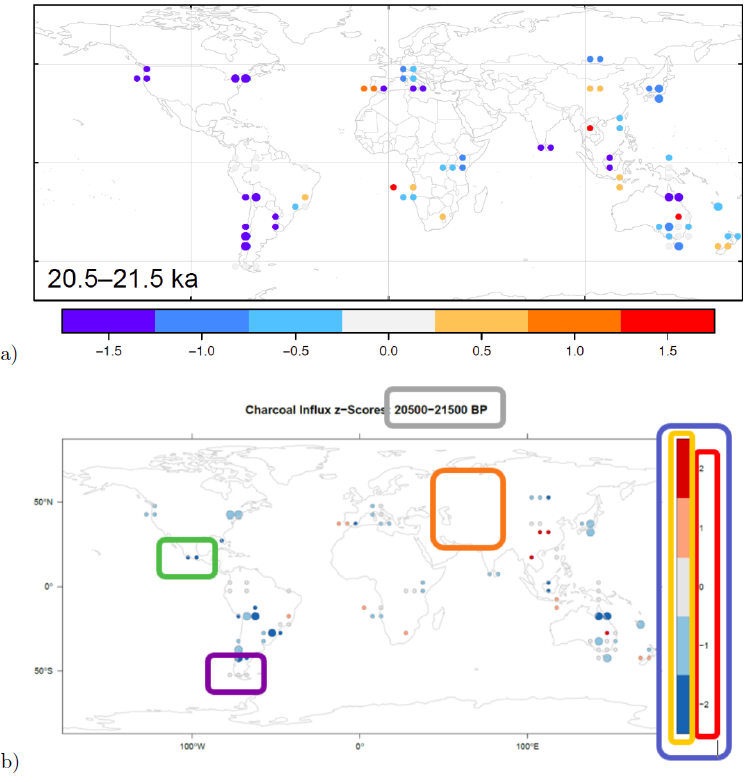
\includegraphics[scale=0.5]{motivation_example}
	\caption{Example of a comparison of the original result (a) and a replicated result (b). The boxes are highlighting the differences of the map. The blue box shows the misplacement of the legend, the purple box shows different colour of results, the red box shows a different data type of the legend numbers, the grey box shows a different labeling, the orange box highlights differences in the background map, the yellow box shows a different number of classes and the green box shows results that were not in the original figure \cite{Thestateofreproducibility}.}
	\label{fig:motivation} % \label has to be placed AFTER \caption (or \subcaption) to produce correct cross-references.
\end{figure} 
\todo{Introduction Status}
% Paper Problem continue





% Old Problem Description



% Old Motivation

%Over the last decades, remote sensing agencies have increased the variations of data processing and therefore, the amount of resulting data. The complexity of the experiments leads researchers to use external services for the workflow. These circumstances make it hard for scientists to provide the necessary information to enable reproducibility. Scientists create a description of the workflow and the used satellite identifier to describe experiments. It is necessary to have citable data and processes on the data to ensure long-term reproducibility to preserve the data for further usage in the future,  \cite{6352411}. 


%\section{Problem Description}\label{Problem}
%The vast majority of data used in earth observation sciences are retrieved and provided via \gls{soa} interfaces. Data providers like \gls{gee}\footnote{https://earthengine.google.com} and \gls{eodc}\footnote{https://www.eodc.eu} host a Web \gls{api} for data download and processing data. These services are used to define the experiment workflow, the definition of the input data, the execution, and the retrieval of the results. Therefore, the researcher is not in full control of the code execution and the environment of their experiments, since the information about the workflow environment of the experiment is not accessible for the scientists. Used external dependencies for processing the earth observation data cannot be accessed. The services act as black boxes to the researchers with no possibility to get versions of the used packages to calculate the resulting images. The situation leads to the problem that researchers are not capable of describing the experiments in a way that they are reproducible. \\
%Input data of a typical remote sensing workflow is satellite data of a specified satellite type filtered by a temporal and a spatial extent. The raw satellite data is preprocessed by the backend provider so that there is a global dataset. Geoscientists using the same satellite identifier could have different results after executing the same experiment if the provider updated the way the data is preprocessed. An example for this is the format update of \gls{esa} in 2017 of the Sentinel 1 dataset, which affected old data records, see \footnote{https://sentinel.esa.int/web/sentinel/missions/sentinel-1/news/-/article/sentinel-1-update-of-product-format}. When scientists use the dataset of a data provider, there is no possibility to see changes in the preprocessing algorithm. Therefore, data versions are not visible to the researcher. The situation leads to the problem that scientists are not capable of identifying the input data, which is a necessity for reproducibility.

%Due to a different range of functionality and a difference between the endpoints of the providers, it is great afford to create a workflow for more than one provider. The openEO project has the goal to be an abstraction layer above different EO data providers. Further information on the software architecture of the project is defined in the project proposal (\cite{openeo}) and in Section \ref{Related Work}. During the creation time of this thesis there is no consideration of repeatability in the openEO architecture. Verification of workflows for users of openEO is not in the agenda of the openEO project. Generalized layers have the opportunity to be implemented in a way that makes processes and data scientifically verifiable and reproducible, as it handles data and processes on the data in a standardized way for different providers. Even though the range of functionality and the API endpoints are well-defined in the openEO core-API, the contributing content providers (openEO backends) will have different underlying software execution environments. The used technology of an openEO backend will evolve in the future, hence it can lead to different results on the same workflow execution. Considering the following: A scientist runs an experiment using openEO as research tool and gets an arbitrary result. The same scientist runs the same experiment with the same input data some months later and gets a slightly different result. The question occurs, why are the results distinct? Has the used data changed, has the user accidentally submitted different code or has some underlying software inside the backend provider changed. Adding a possibility for the users of openEO to gain this information is an important feature for the scientific community. The aim of this thesis is to design an extension to openEO, so that users are able to retrieve provenance data about a job re-execution \cite{openeo}. 

\section{Aim of the Work}\label{Aim}\label{Use Cases}
\todo{Standalone Section with only the Research Questions}
The following sections define the use cases to validate the design proposed in this thesis. They describe scenarios focused on scientific workflows that are currently not achievable, but shall be accomplish-able with the solution of this thesis. This thesis uses the term "job" for the definition of workflow since it is common in earth observation science.

\subsection{Example Experiment}\label{example}

This section describes an example of an experiment that a remote sensing scientist wants to execute. The thesis uses the example throughout the thesis for a better illustration of the concepts. The following sections use it for the Use Cases. \\
The input data of the experiment is Sentinel 2 data developed by the European Space Agency (ESA). The area of interest is the province of South Tyrol. More specifically the bounding area in the "EPSG:4326" projection with the coordinates for a north-west corner of (10.288696, 46.905246) and a south-east corner of (12.189331, 45.935871). The time of interest is the month of May of the year 2017. In this example, the scientist is working on vegetation dynamics and wants to know what the state of the vegetation of South Tyrol was in May of 2017. Therefore the minimum of the  \gls{ndvi}\footnote{https://earthobservatory.nasa.gov/features/MeasuringVegetation/measuring\_vegetation\_2.php} is calculated on the data selection. It derives from the difference between near-infrared (which reflects vegetation strongly) and red light (which vegetation absorbs). So for every pixel of the satellite image, the NDVI value is calculated for every day of May 2017. Then the 31 images for May 2017 are reduced to one by taking the minimum NDVI value of each pixel. Figure \ref{fig:example} shows the result of the running example execution.\\

The execution of the experiment consists of the following steps:

\begin{enumerate}
	\item Selecting the Sentinel 2 data records
	\item Filtering the Sentinel 2 records by the extent of south tyrol. \\(10.288696, 46.905246) - (12.189331, 45.935871) on "EPSG:4326" projection.
	\item Filtering the Sentinel 2 records by May 2017.
	\item Calculate NDVI for all days of May 2017.
	\item Reduce by the minimum value of May 2017.
	\item Interpret the resulting image.
\end{enumerate}

\begin{figure}[h]
	\centering
	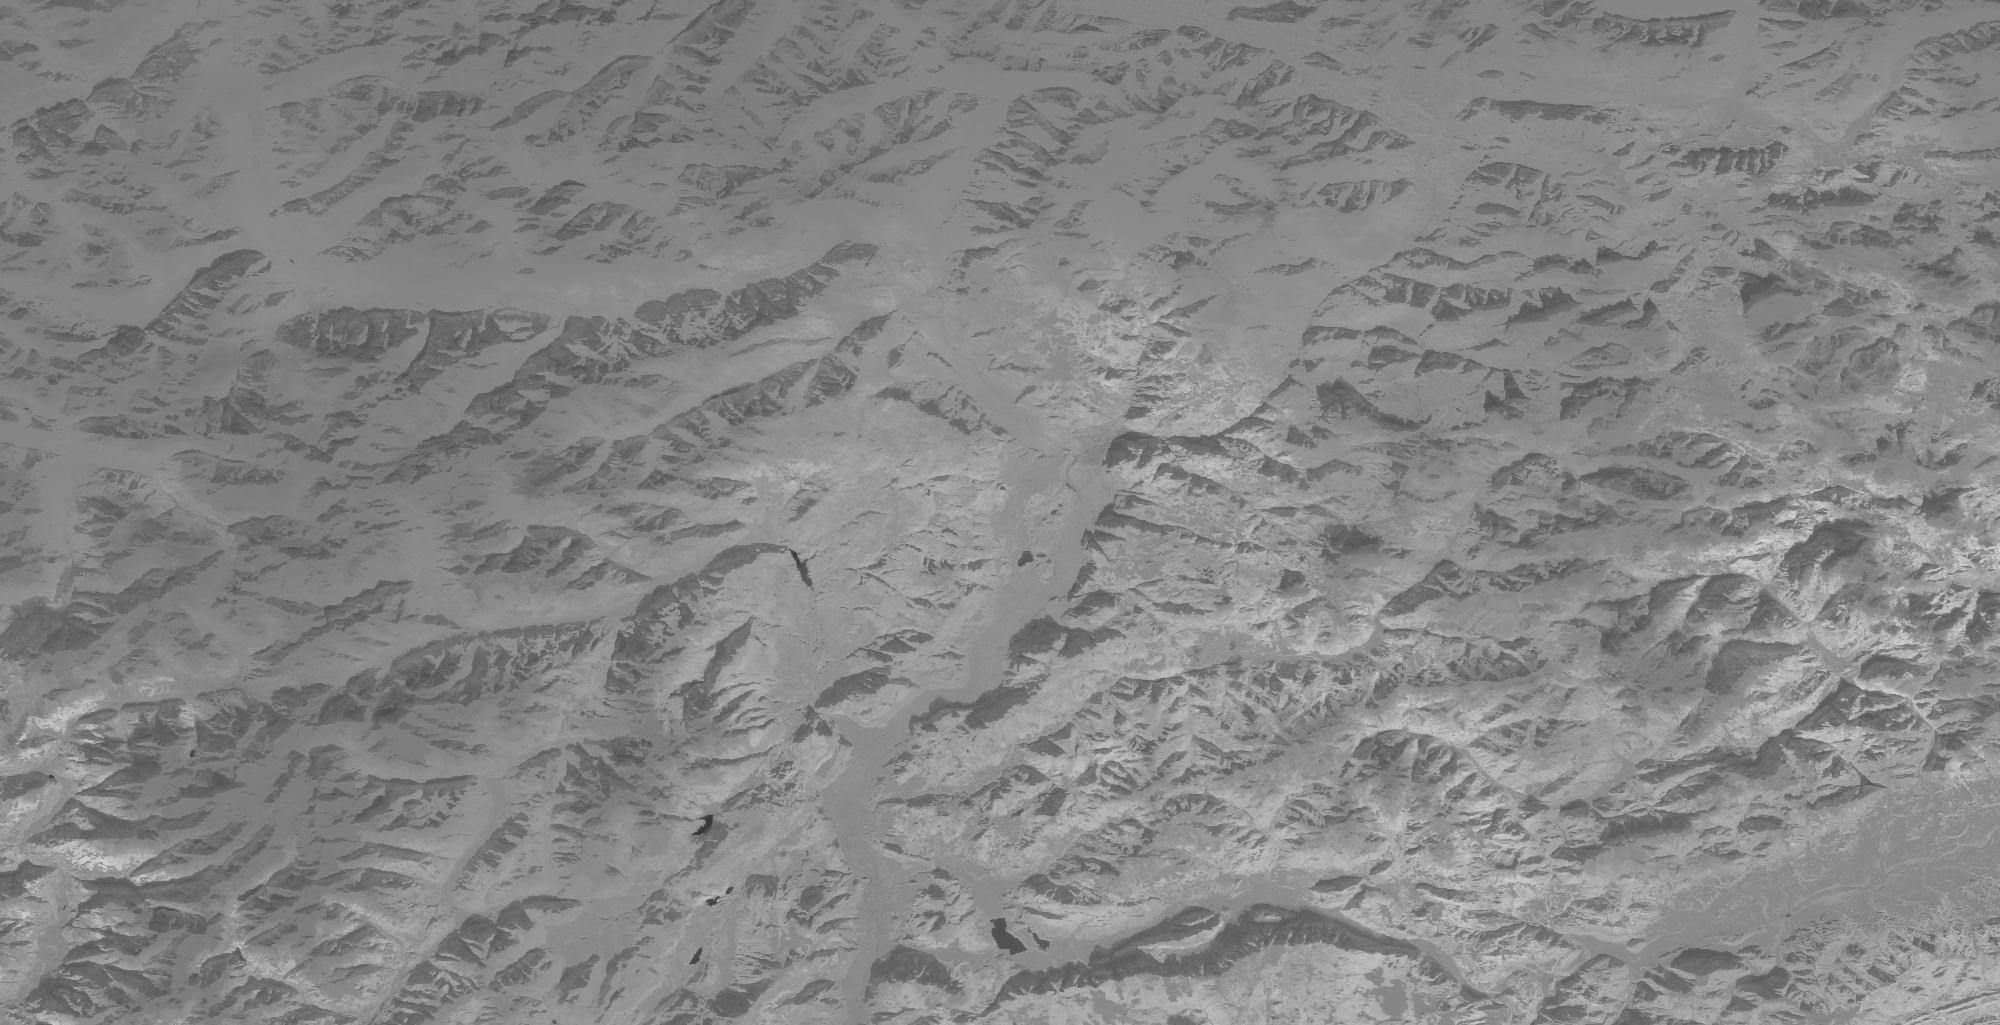
\includegraphics[width=\textwidth]{openeo_example_output}
	\caption{Resulting image of the running example.}
	\label{fig:example} % \label has to be placed AFTER \caption (or \subcaption) to produce correct cross-references.
\end{figure}


\subsection{Use Case 1 – Re-use of input data}\label{UseCase1}
\begin{figure}[h]
	\centering
	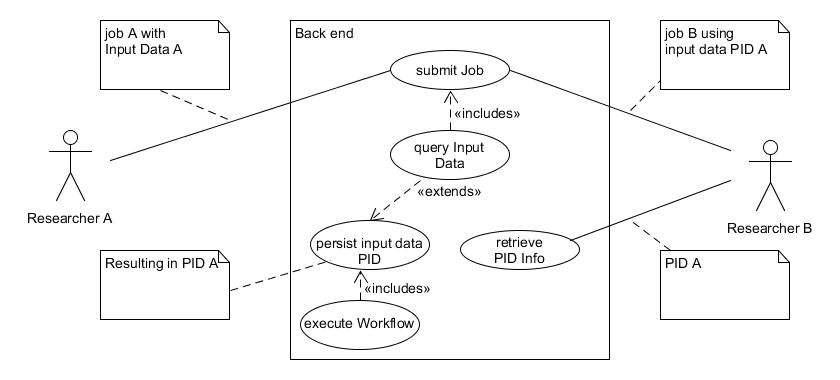
\includegraphics[width=\textwidth]{usecase1}
	\caption{Overview of the first Use Case.}
	\label{fig:usecase1} % \label has to be placed AFTER \caption (or \subcaption) to produce correct cross-references.
\end{figure}
The first use case is about the re-use of input data between job executions. Reproducible methods are especially important for the scientific community. Since scientists are likely to build on results and methods of publications, this is a scenario to make the re-use simpler. In this case, a scientist wants to create a publication by running the example, described in Section \ref{example} on an earth observation backend. The backend generates a \gls{pid} for the input data of the experiment. After that, the scientist publishes the results and cites the input data with the resulting PID. The PID redirects to a human-readable landing page that provides meta information about the dataset. Another scientist also interested in the vegetation of South Tyrol wants to use the same input data but chooses a different approach of processing it (for example the maximum instead of minimum). Hence, the input data PID can be used to re-use the same data. The backend has to be capable of resolving the PID automatically to let the user work with the same input data for a new workflow. The data provider needs to persist the data defined by a PID even if the preprocessing of the data changes in the future.   

\begin{itemize}
	\item \textbf{Input Data A}: Sentinel 2 data of the area of South Tyrol in May 2017. 
	\item \textbf{Job A}: Taking the \textbf{minimum} NDVI of the area of South Tyrol in May 2017. 
	\item \textbf{Job B}: Taking the \textbf{maximum} NDVI of the area of South Tyrol in May 2017.
\end{itemize}

Figure \ref{fig:usecase1} gives an overview of the use case. \\

The scenario sequence of actions is summarized in the following steps: \\

\begin{enumerate}
	\item Researcher A runs job A at the backend.
	\item Researcher A retrieves the used input data PID of job A.
	\item Researcher A cites the input data with the PID in a publication.
	\item Researcher B uses the same input data, by applying the data PID of job A for job B.  
\end{enumerate}

\subsection{Use Case 2 – Providing job execution Information}\label{UseCase2}
\begin{figure}[h]
	\centering
	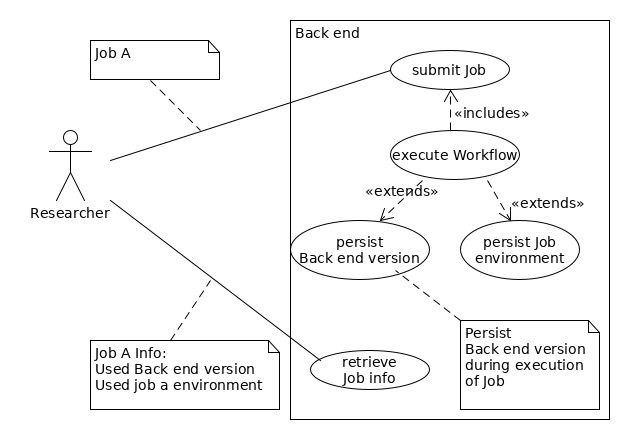
\includegraphics[width=\textwidth]{usecase2}
	\caption{Overview of the second Use Case}
	\label{fig:usecase2} % \label has to be placed AFTER \caption (or \subcaption) to produce correct cross-references.
\end{figure}

The second use case is like the first one but is exclusively about job dependent environment information. The scientist can automatically get environment data about the job execution e.g. used software packages and their versions. The motivation for this is to add transparency to the job processing for the users so that researchers can describe their processes in more detail. It can help geoscientists to understand why results differ from executions in the past. Figure \ref{fig:usecase2} gives an overview of the use case. 
The following steps summarize the scenario sequence of actions: \\
\begin{enumerate}
	\item Researcher runs an experiment (job A) at a backend.
	\item Researcher wants to describe the experiment environment.
%	\item Back End Developer releases a new version.   
%	\item Back End Developer runs test jobs to find differences.
\end{enumerate}

\subsection{Use Case 3 – Compare different job executions}\label{UseCase3}
\begin{figure}[h]
	\centering
	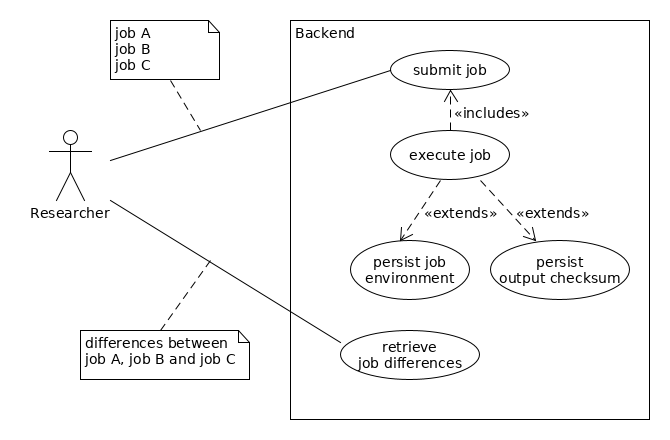
\includegraphics[width=\textwidth]{usecase3}
	\caption{Overview of the third Use Case}
	\label{fig:usecase3} % \label has to be placed AFTER \caption (or \subcaption) to produce correct cross-references.
\end{figure}
The third use case dedicates to the comparison of job executions. The goal is to add a possibility for geoscientists to compare different jobs not only by their results but on the way they are executed. The same backend applies the comparison between a job execution and another job execution. Therefore, the processing implementation and the input data has to be identifiable. To make the comparison enjoyable to the users, additional data is added to the job environment data e.g. an output checksum. For usability reasons, the comparison needs to be easy to apply and easy to understand, therefore accessible in the context of the user. In addition to the previous conditions, a visualization of the differences for the users can lower the access barrier for them to use the feature. Figure \ref{fig:usecase3} gives an overview of this use case.
The following steps summarize the scenario sequence of actions: \\

\begin{itemize}
	\item \textbf{Job A}: Taking the minimum NDVI of the area of South Tyrol in May 2017. 
	\item \textbf{Job B}: Taking the minimum NDVI of the area of South Tyrol in May 2017.
	\item \textbf{Job C}: Taking the maximum NDVI of the area of South Tyrol in May 2017.
\end{itemize}

\begin{enumerate}
	\item Researcher runs an experiment (job A) at a backend.
	\item Researcher re-runs the same experiment (job B).
	\item Researcher runs a different experiment (job C).   
	\item Researcher receives a comparison of the jobs (A, B, C) by their environment and outcome.
\end{enumerate}

\subsection{Research Questions}\label{research question}
\todo{Use propose in the first sentence --> Done}
\todo{Use Accessible instead of available}
\todo{Two objectives: Capturing, Make Accessible}
\todo{Do not use implement that often here, it is not so important --> the Model is the important thing in the thesis}
\todo{contribute to openEO project to provide information on reproducibility}
\todo{openEO just sets the context}
\todo{At least big questions: How --> What}
\todo{RQ1 --> Mention Repeated, What Information...about environment...}
\todo{Generell: Software --> Environment}
\todo{RQ1.2 --> not software}
\todo{RQ1.3 --> maybe remove or rename --> Where to put the stuff to capture --> See Conclusion}
\todo{Reminder: PROV-O ? Andi didn't notice ...}
The expected outcome of this thesis is to propose a framework for making repeatability conceivable in the earth observation community. The solution enables users to re-execute workflows and validates the result, so that differences in the processing or the data are accessible for the users. To achieve this goal, a model for capturing the environment of the backends has to be discovered and implemented. Since the solution is implemented within the \gls{openeo} (details see Section \ref{openEO}), it shall conclude in recommendations for the openEO project on how to improve re-execution validation for the users and how it is achievable. Considering the problem description and the scenarios above, the following research questions can be formulated:

\begin{itemize}
	\item \textbf{How can an earth observation job re-execution be applied like the initial execution?}
	\begin{itemize}
		\item How can the used data be identified after the initial execution?
		\item How can the used software of the initial execution be reproduced?
		\item What data has to be captured when?
		\item How can the result of a re-execution in future software versions be verified?
	\end{itemize}
	\item \textbf{How can the equality of a earth observation job re-execution results be validated?}
	\begin{itemize}
		\item What are the validation requirements?
		\item How can the data be compared?
		\item How can changes of the earth observation backend environment be recognized?
		\item How can differences in the environment between the executions be discovered?
	\end{itemize}
\end{itemize}

\section{Methodological Approach}\label{Method}
The use cases defined in the previous section require specific changes to the components of an earth observation backend. The following list describes the parts of the suggested solution: 
\todo{Revisit and rewrite it...}

\begin{enumerate}
	\item \textbf{Data Identification}
	The input data has to be identifiable, to accomplish the capturing of processing workflows described in the use cases in Section \ref{Use Cases}. To achieve this, the recommendations of the \gls{rda} (see \cite{rauber2016identification}) have to be implemented by adding versioning and query databases.
	
	\item \textbf{Process Versioning}
	The process has to be identifiable, to accomplish the verification of different process executions. Therefore, the versioning of the process code can be used to persist states of the code. The thesis is for an open source project, and the code of the backends are published at Github, so we use Git as the tool to capture the code state. 
		
	\item \textbf{User Endpoints}
\todo{Change text to openEO contibution}
	The interface for users has to be implemented so that the use cases can be executed. Therefore, client applications have to be modified. The used programming language in this thesis is Python\footnote{https://www.python.org}.
\end{enumerate}

\section{Structure of Work}\label{Structure}
The following chapters are structured as followed:\\
Chapter 2 gives an overview of related scientific activities in the area of reproducibility in the earth observation sciences and reproducibility in other areas with similar objectives. \\
%Chapter 3  describes the technologies and concepts that are used in the implementation of this thesis. This chapter provides an overview of the EODC backend used for the implementation.\\
Chapter 3 provides the concept to address the research questions defined in Section \ref{Aim}.  This is the theoretical definition of what has to be implemented in the openEO project.\\
Chapter 4 has a detailed explanation to the proof of concept prototype implementation and how the concept of chapter 3 was realized for the EODC backend. \\
Chapter 5 dives into the evaluation of the implementation by applying test cases to the implementation of chapter 4.\\
Chapter 6 summarizes the outcome of the implementation and evaluation. It contains a discussion on results achieved, open issues and future work. \\

\chapter{Related Work}\label{Related Work}

\todo{Gesamte Thesis: Present simple \& Past simple and not "could / would" So: we have implemented --> we implemented}
\todo{Gesamte Thesis: Restructure passive sentences}
\todo{Gesamte Thesis:Konsistente Verwendung von Begriffen --> Glossary ?? --> workflow (Beschreibung des Experiments aus sicht des wissenschaftlers), job (Definition des im backend durchgeführten parts), workflow, process graph (technische Beschreibung bzw. Definition des jobs)}
\todo{Gesamte Thesis: Wortwiederholungen sind gut !!}
\todo{Gesamte Thesis: Unnötige Wörter / Sätze weg z.b. briefly, some, also, ...}
\todo{Gesamte Thesis: Kurze einfache Sätze}
\todo{Gesamte Thesis: Eher Reproducibility schreiben in den Allgemeinen Kapiteln, aber in den RQ repeatability schreiben}
\todo{Gesamte Thesis: Software --> Environment / Code ? --> just check correct usage}

This chapter describes the related work that influenced this thesis. It informs the reader about concepts related to the proposed solution. The information is structured in subsections, each representing important technologies or concepts in the context of this thesis. \\The first section presents the concepts behind reproducibility in computer science. \\
The second section describes the state of reproducibility in earth observation science. \\
The third section presents concepts related to data identification. \\ 
The fourth section consists of other existing implementations to achieve reproducibility. \\
The last section of this chapter describes the openEO project and the EODC backend, which we use for the proof of concept implementation in Chapter \ref{Implementation}.      


\section{Reproducibility}\label{Reproducibility}
The term of reproducibility is defined as a new experiment based on an original experiment by an independent researcher in the manner of the original experiment. Reproducibility aims to gain additional evidence on the result of the original result by creating an independent experiment that shows similar results. Repetition defines a re-run of the same experiment with the same method, same environment, and a very similar result. The repetition aims to check if the methods described in a publication are resulting in the purposed outcome \cite{6064509}. 
Achieving reproducibility is a common problem in all scientific areas. Therefore there are ten rules defined to gain a common sense about reproducibility. They are motivated by the basic idea that every result of interest has to be associated with a used process and data. The researcher has to provide external programs as well as custom script versions. Using version control software is recommended. Besides, one of the steps defines a rule to make scripts and their results publicly available \cite{10.1371/journal.pcbi.1003285}. 
Reproducibility is the crucial topic of The Fourth Paradigm. It leads to the term eScience, which has the aim of bringing science and computer technologies closer together. The general concept is to enable scientific procedures with new information technologies used by data-intensive sciences. The expected result of eScience is to get all scientific papers publicly available, including the necessary data and workflows, so that scientists can interact more efficiently \cite{noauthororeditorfourth}. 
eScience has the potential to enable a boost in scientific discovery. It provides approaches to make digital data and workflows citable. The publication \cite{Rauber2015RepeatabilityAR} discusses a general way of reaching this. It describes an approach to look at whole research processes by introducing Process Management Plans, other than limiting it to data citation. It demonstrates the capturing, verification, and validation of the input data for a computational process.
Computer sciences have the issue of high amounts of published papers that do not provide enough information to make them reproducible. This is not solved by the scientists that need to make additional effort, but by providing new tools for scientists that allow it automatically  \cite{MIKSA201725}. There are some additional issues on reproducibility in computer science e.g. in the case that used software technologies are deprecated and not available anymore. Therefore, persisting the execution context is needed to achieve a re-execution of the experiment. One proposed solution is the VFramework described in more detail in Section \ref{vframework}. 
The PRIMAD model defines a set of variables that define an experiment. The relationship of the original execution to a re-execution is visualized by noticing changes in the variables. The following variables of an experiment are used to describe the relationship \cite{primad}:

\begin{itemize}
	\item \textbf{P} Platform / Execution Environment / Context (e.g. Python 2.7, Windows 10,\dots) \\
	\item \textbf{R} Research Objectives / Goals (e.g. sorting the input) \\
	\item \textbf{I} Implementation / Code / Source-Code (e.g. script in Python) \\
	\item \textbf{M} Methods / Algorithms (e.g. quick sort) \\
	\item \textbf{A} Actors / Persons (e.g. researcher that is executing the experiment) \\
	\item \textbf{D} Data (input data and parameter values)   (e.g. input data that is to be sorted) 
\end{itemize}

If there is a re-execution that is different on every variable to the original one, except for the same method (M) and goal (R), it is considered a reproduction \cite{primad}. 
\\  
Data citation is a vital issue of reproducing results of past experiments. Preserving the exact workflow without persisting the original data has no positive effect on the scientific community. If the data used in an experiment is not available anymore, or not specified explicit enough, then there is no chance of reproducing it no matter how much information about the execution is known. In earth observation persisting the data for reproducibility in the future is an issue discussed in the literature \cite{6352411}. Gaining data identification in digital sciences has an official working group named \gls{wgdc}, which created 14 recommendations on data citation further explained in Section \ref{Data Identification}.

 \subsection{PROV-O}\label{PROV}
In 2003 the World Wide Web Consortium published the PROV model as a standard concerning provenance definitions. It is defined in twelve documents. In the context of this thesis the PROV Ontology (PROV-O) is the most relevant \cite{733f89c65e4844f9aabcae1c276a5602}. 
PROV-O is a standard language using OWL2 Web Ontology. It is a lightweight concept capable of a broad spectrum of applications.  

\begin{figure}[h]
	\centering
	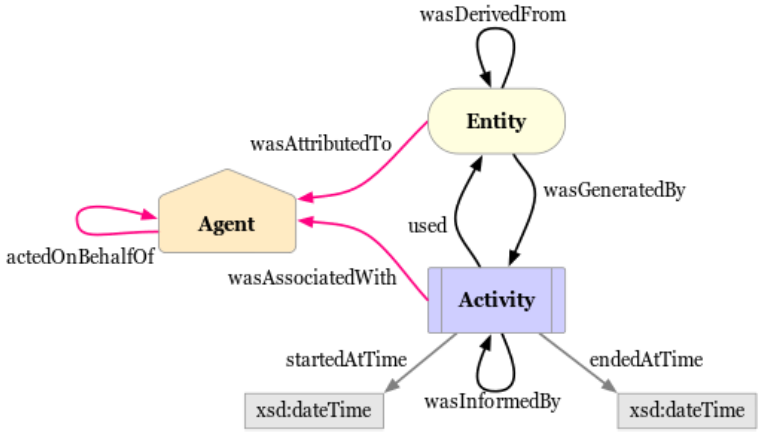
\includegraphics[scale=0.6]{prov}
	\caption{Overview of the main components of PROV-O \cite{733f89c65e4844f9aabcae1c276a5602}}
	\label{fig:prov} % \label has to be placed AFTER \caption (or \subcaption) to produce correct cross-references.
\end{figure}

Figure \ref{fig:prov} shows the basic setup of the PROV-O concept. It consists of three main elements. The \textit{Entity} is any physical, digital or conceptual thing. Provenance records describe \textit{Entities} that can consist of references to other \textit{Entities}. Another element is the \textit{Agent}, which is responsible for \textit{Activities} and that they are taking place, e.g. software, persons, or organizations. The association of an \textit{Agent} to an \textit{Activity} defines the responsibility of the \textit{Agent} for the \textit{Activity}. An \textit{Activity} describes what happened that the \textit{Entity} has come to existence and how attributes of an \textit{Entity} changed \cite{733f89c65e4844f9aabcae1c276a5602}. The design chapter \ref{Design} does not specify the representation of the context information. Therefore the PROV ontology can be used to represent the information. This thesis is not implementing the PROV-O standard since the EODC backend providers wanted their representation of it, which is an extension of the existing data representation, but it is a reasonable extension. 

\subsection{VFramework}\label{vframework}

The VFramework defines parallel capturing of provenance data during the workflow execution. During the original execution, evidence gets collected into a repository e.g. logging. The context model of the execution persists the needed data e.g. in a database record. Re-execution is verified and validated using the provided provenance data in the context model of the original execution and the context model of the re-execution. The provenance data divides into static and dynamic data. Static data defines data that is not dependent on the execution of the experiment e.g. the operating system and installed packages. The static environment information is, therefore, independent of the configuration of the workflow. Dynamic data is captured during the execution of the original experiment e.g. python version of the execution or used input files. It describes data dependent to a workflow execution \cite{Miksa2013FrameworkFV}. 
Figure \ref{fig:vframework} shows an overview of the VFramework concept described above.   
\begin{figure}[h]
	\centering
	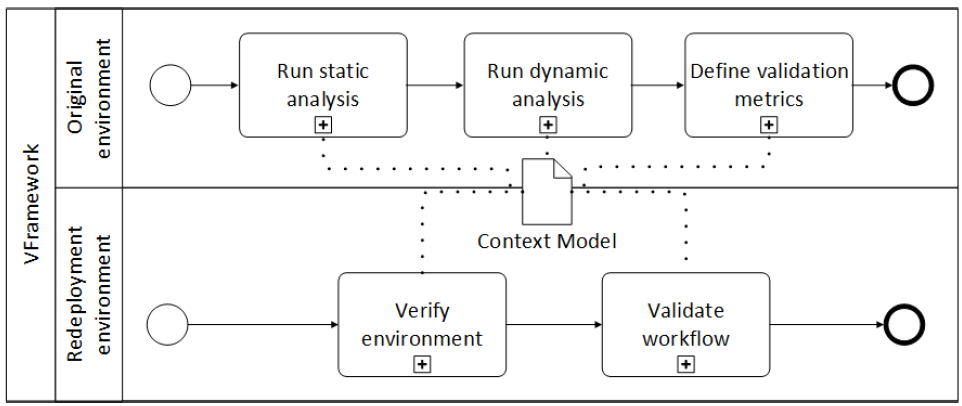
\includegraphics[width=\textwidth]{vframework}
	\caption{Overview of the Concept of the VFramework \cite{Miksa2013FrameworkFV}}
	\label{fig:vframework} % \label has to be placed AFTER \caption (or \subcaption) to produce correct cross-references.
\end{figure}

\section{Earth Observation Science}\label{EOScience}

This section describes Reproducibility in the context of the computational geoscience. A study tests the reproducibility and replicability of scientific papers in geoscience by obtaining more than 400 papers \cite{Ostermann2017AdvancingSW}. In \cite{Ostermann2017AdvancingSW} a reproduction is defined by an exact duplicate of an experiment, whereas it defines replication as a resemblance of the original execution, but allowing variation e.g. different scales. Table \ref{Tab:geoprimad} describes the difference between reproduction and replicability in PRIMAD terms. Since the definition of the paper differs from the definition of this thesis the terms are marked as Reproducibility' and Replicability'. Only half of the test group publications are replicable, and none of them reproducible. There are publications to address the lack of reproducibility in the earth observation science. The following sections summarize these concepts.     

\begin{table}[]
	\caption{PRIMAD description of reproduction and replication according to \cite{Ostermann2017AdvancingSW}}
	\begin{tabular}{l|l|l}
		 & \textbf{Reproduction'} & \textbf{Replication'}  \\ \hline
		\textbf{P}latform & same & different \\ \hline 
		\textbf{R}esearch Objectives & same & same \\ \hline  
		\textbf{I}mplementation  & same & different  \\ \hline  
		\textbf{M}ethods & same & different \\ \hline 
		\textbf{A}ctors & different & different \\ \hline
		\textbf{D}ata & same & different, but similiar \\ \hline
	\end{tabular}
	\label{Tab:geoprimad}
\end{table}
\todo{Related Work Status}
\subsection{Vadose Zone Journal (VZJ)}\label{VZJ}
In order to face the issue of lacking reproducibility in geoscience the \gls{vzj} started a \gls{rr} program in 2015 \cite{doi:10.2136/vzj2015.06.0088}. 
The earth observation science is a big part of VZJ publications, and most of them are not applying the open computational science guidelines. The main reasons are behaviors of scientists that do not see the overall benefit of putting effort into documentation. Therefore, the VZJ started an RR program to publish alongside the scientific paper the code and data used by the scientists for evaluating the publication. The strategy shall lower the access barrier for scientists to publish their research work entirely. Aim of the project is to create a community of researchers with a shared sense of reproducibility and data citation on the platform and to animate other scientists to join the approach. On time this thesis is written, the service is still available\footnote{https://dl.sciencesocieties.org/publications/vzj/author-instructions-reproducible-research}, but there were no results available on how much it is used \cite{doi:10.2136/vzj2015.06.0088}.

\subsection{The Geoscience Paper of the Future (GPF)}\label{GPF}

The geoscience paper of the future (GPF) is according to \cite{Gil2016TowardTG} a proposed standard to help geographical scientists by making reproducible publications. It defines recommendations on data management and software management by introducing the reader to available repositories. The gain of it is applying concepts of open science and reproducibility to earth observation papers. A GPF needs to apply the following requirements:

\begin{itemize}
	\item \textbf{Reusable data} in a public repositories and persistent identifiers.
	\item \textbf{Reusable software} (including software for preparing and post editing of the data) in a  public repositories and persistent identifiers.
	\item \textbf{Documenting the computational provenance of results} in a public repositories and persistent identifiers.  
\end{itemize}

\begin{figure}[h]
	\centering
	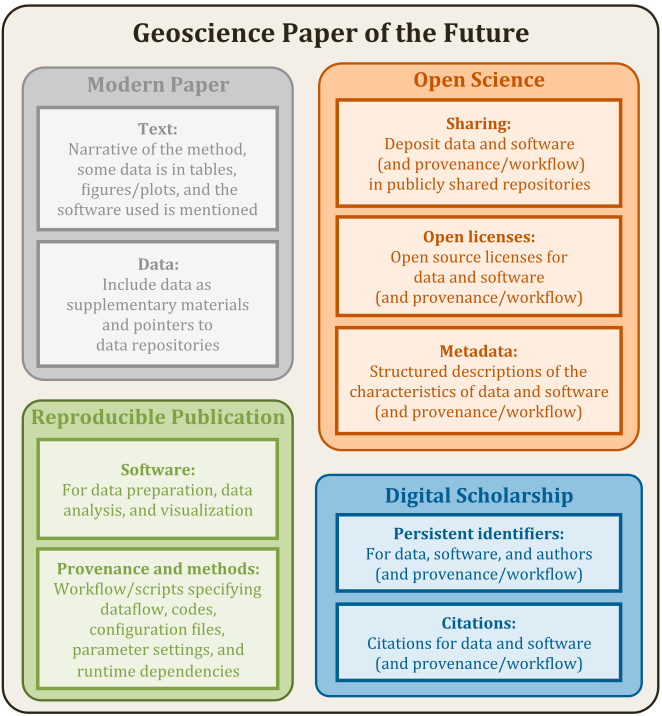
\includegraphics[scale=0.5]{gpf}
	\caption{Comparison between reproducible publications and geoscientific papers of the future \cite{Gil2016TowardTG}}
	\label{fig:gpf} % \label has to be placed AFTER \caption (or \subcaption) to produce correct cross-references.
\end{figure}

Figure \ref{fig:gpf} visualizes the differences with a reproducible paper. In addition to the characteristics of the reproducible paper, the GPF focuses on publishing the data publicly with open licenses with citable persistent identifiers.
The GPF consists of a set of 20 recommendations for geoscientists regarding data accessibility, software accessibility, and provenance information. GPF authors may find reasons not to be able to follow the rules and therefore, have to find workarounds and propose areas for future improvements. The strategy of the GPF community is to educate the scientist to make reproducible publications, by making training sessions for them\footnote{http://scientificpaperofthefuture.org/gpf/events.html}, instead than providing tools to make it easier for scientists to use it. In comparison to this thesis, it is a different approach to achieve the same goal; in this thesis, the strategy is to achieve reproducibility in geoscience through technology. 

\subsection{Climate Change Centre Austria (CCCA)}

The \gls{ccca} is a research network for Austrian climate research online available since 2016 and has 28 members. The main tasks are the provision of climate-relevant information, the inter-operable interfaces, and long term archiving of scientific data. In 2017 the \gls{netcdf} data citation was added to the project. The set up of the data service and the technology used in the background is similar to the set up of the EODC backend. Therefore, the process of enabling data identification was similar to this thesis. CCCA is Open-source and available at GitHub, see the GitHub repository\footnote{https://github.com/ccca-dc}. The concept used for gaining data citation was the RDA recommendations defined in \cite{rauber2016identification}. Figure \ref{fig:ccca} shows an overview of the CCCA implementation. It uses a ckan\footnote{https://ckan.org} web server to handle the request and responses of the user, which are then passed to a python application. The python part is responsible for the query store functionality. The core element is the \gls{tds}\footnote{https://www.unidata.ucar.edu/software/thredds/current/tds/}, which is responsible for the actual data archive.   
The python application part of the CCCA overview is similar to the implementation of this thesis. The main difference is the objectives of the CCCA service compared to the EODC backend. On the CCCA platform, any climate-relevant information (e.g. air temperature or frost days) can be uploaded and persisted. On the EODC backend, preprocessed global earth observation data is persisted, which is used as input data for processing chains. Therefore, the data on EODC is more homogeneous than the data on the CCCA platform.
Nevertheless, the concept of enabling data identification is similar in both projects. The CCCA implementation inspired the query store implementation of this thesis. The query result differs, because EODC uses \gls{geotiff} instead of NetCDF at their backend. Another difference is that CCCA uses HTTP GET requests as query, whereas the EODC backend uses \gls{xml} based queries, which are also limited by the openEO API specification  \cite{ccca}.  

\begin{figure}[h]
	\centering
	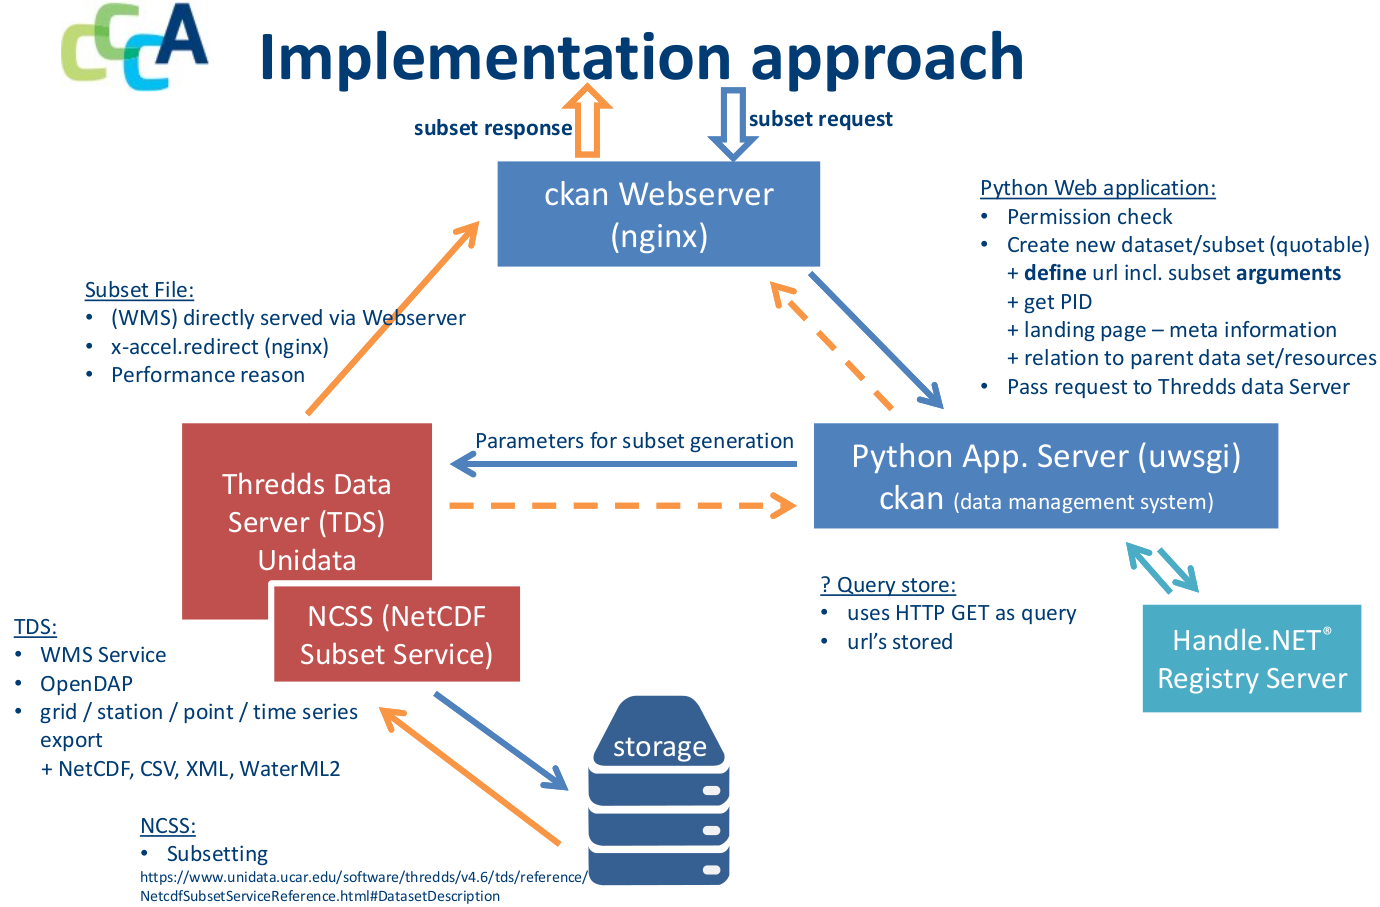
\includegraphics[scale=0.25]{ccca}
	\caption{Concept of the CCCA NetCDF Cata Citation}
	\label{fig:ccca} % \label has to be placed AFTER \caption (or \subcaption) to produce %correct cross-references.
\end{figure}

\section{Data Identification}\label{Data Identification}

Data identification and citation is the main concern in many computers relying on sciences. For the aim of this work, the input data is a key element of the capturing. If the input data can not be identified correctly, the capturing of the processing on it does not gain useful information. Therefore the identity of the data has to be guaranteed. The Research Data Alliance (RDA) presents general solutions to achieve data identifications. There are 14 recommendations defined to achieve the identification of an exact version and subset of input data. The recommendations are independent of the type of data and database system. In the following the recommendations are summarized \cite{rauber2016identification}.

\begin{itemize}
	\item \textbf{R1: Data Versioning} \\
	Changes on a data record must result in a new version of the data record and the persistence of the deprecated data records. All data record versions have to be identifiable and accessible. 
	\item \textbf{R2: Timestamping} \\
	All changes to the database have to be comprehensible via timestamps. Every time changes are applied to the data, there has to be a time stamp persisted to describe when it happened. 
	\item \textbf{R3: Query Store Facilities} \\
	There has to be a query store implemented at the data provider to store queries including their data, to be able to re-execute them in the future. The database has to store, according to \cite{rauber2016identification}, the following things: 
	\begin{itemize}
		\item The original query as applied to the database
		\item A potentially re-written unique query created by the system (R4, R5)
		\item Hash of the (unique) query to detect duplicate queries (R4)
		\item Hash of the result set (R6)
		\item Query execution time stamp (R7)
		\item Persistent identifier of the data source
		\item Persistent identifier for the query (R8)
		\item Other data (e.g. author or creator information) required by the landing page (R11)
	\end{itemize}
	\item \textbf{R4: Query Uniqueness} \\
	Since it is not desirable to have equal queries with the same result stored at the query store, there needs to be a normalized query that can be directly compared to other queries. Hence, there needs to be an algorithm to normalize the queries and to guarantee their uniqueness.
	\item \textbf{R5: Stable Sorting} \\
	The sorting of the resulting data has to be unambiguous if the sequence of data item presentation is essential for the reproduction.
	\item \textbf{R6: Result Set Verification} \\
	To ensure that the resulting data of the query is comparable there have to be a checksum or hash key of it. 
	\item \textbf{R7: Query Timestamping} \\
	There has to be a time stamp assigned to every query in the query store, which can be set to the latest update of the entire database, or the query dependent data of the database, or simply the time of query execution.
	\item \textbf{R8: Query PID}\\
	Every query record in the query store must have a Persistent Identifier (PID). There should not be a query with the same normalized query and the same query result checksum. 
	\item \textbf{R9: Store the Query} \\
	The data described in previous recommendations have to be persisted in the query store.
	\item \textbf{R10: Automated Citation Texts} \\
	To make the citation of the data more convenient for researchers, there shall be a automatic generation for the citation text snipped containing the data PID.
	\item \textbf{R11: Landing Page} \\
	The PID shall be resolvable in a human readable landing page, where data mentioned in the previous recommendations is provided to the scientist.
	\item \textbf{R12: Machine Actionability} \\
	Providing an API landing page so that not only humans, but machines can access the data by resolving the PID.
	\item \textbf{R13: Technology Migration} \\
	If the database where the query store is implemented needs to be migrated to a new system, the queries need to be transferred too. In addition the queries have to be updated according to the new setup, so that they still work exactly like in the old system.
	\item \textbf{R14: Migration Verification} \\
	There shall be a service to verify a data and query migration (see R13) automatically, to prove that the queries in the query store are still correct. 
\end{itemize}
The implementation of the recommendations for the purpose of this thesis is described in Section \ref{Implementation:Data Identification}. Section \ref{Evaluation:dataidentification} shows the evaluation of the data identification implementation. 

\section{Tools for Reproducibility}\label{Existing Tools}
The section describes tools that are designed to solve similar problems or subproblems that are addressed by this thesis. There is an explanation of why the specific tool was not used for the prototype of this thesis or how it was used in parts of the solution. 

\subsection{noWorkflow}\label{Noworkflow}
noWorkflow is introduced in \cite{c9e0604becba42af96a9cb0a6f60018b} as a script provenance capturing tool with the aim to not influence the way researchers implement experiments. As proof of concept, the noWorkflow command line tool got implemented for python. The provenance is captured in an SQLite database by different trials. A trial represents the environment information of one execution. The main benefit of noWorkflow is that it does not instrument the code, and it automatically captures the definition, deployment, and execution environment in a local SQLite database.  The command line interface of noWorkflow is capable of providing access to the stored data. In addition to just retrieving the information about the execution environment, analyses features are added \cite{c9e0604becba42af96a9cb0a6f60018b}.

\begin{figure}[h]
	\centering
	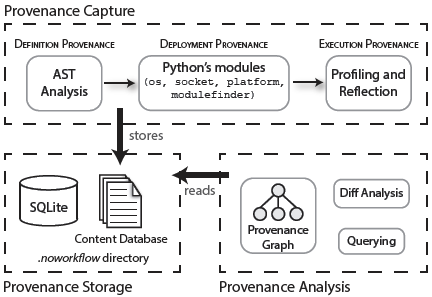
\includegraphics[scale=1]{noworkflow}
	\caption{Architecture of noWorkflow \cite{c9e0604becba42af96a9cb0a6f60018b}}
	\label{fig:noworkflow} % \label has to be placed AFTER \caption (or \subcaption) to produce correct cross-references.
\end{figure}

The noWorkflow framework got improved regularly after the first announcement. Next, an additional feature of tracking the evolution of the experiment executions is added \cite{Pimentel2016TrackingAA}. It improves the possibility to compare different trials of an experiment and to visualize the history of past executions. In \cite{Pimentel:2016:FPC:3090188.3090214} the fine-grained provenance tracking extension of noWorkflow is introduced. With it, the execution of the python script can be viewed as a set of execution lines. It adds a visualization of all called functions with the exclusion of calls in one line on complex data structures such as dictionaries, lists, and objects. In \cite{69bac1252a684629baa43b48e350068d} the provenance capturing of noWorkflow in combination of yesWorkflow, which gathers information about the provenance using comments and annotations (see \cite{192094}), got combined. The combination enabled more detailed environment information, querying, and visualizations. 
In this thesis, noWorkflow was used in an early attempt for the implementation but is not part of the final solution due to the high amount of the captured data by noWorkflow and the additional requirements needed by the EODC backend for using it.

\subsection{ReproZip}\label{ReproZip}
ReproZip is a packaging tool to enable the reproducibility of computational executions of any kind. It automatically tracks the dependencies of an experiment and saves it to a package that can be executed on another machine by ReproZip. It is even capable of letting the re-executor modify the original experiment. It was developed for the SIGMOD Reproducibility Review. In Figure \ref{fig:reprozip}, the architecture of ReproZip is shown in detail. It traces the system calls to create a package defined in the configuration file. Thus, a single file with the extension “.rpz” gets produced. These type of files can then be unpacked on a different machine and re-executed. ReproZip aims to make reproducible science easy to apply for single experiments \cite{29c5846926a4497d95f276604cb0368c}. The reason why it is not used in the solution of this thesis is that the capturing is very fine granulated and takes too much performance from the backends, which is a key selling point for backend providers. Depending on the backend, the payment for users may be dependent on the duration time of the processing. Another issue with ReproZip in the context of this thesis is that it is not capable of capturing the big data of the backends within the package, because it would take too much space and performance.   

\begin{figure}[h]
	\centering
	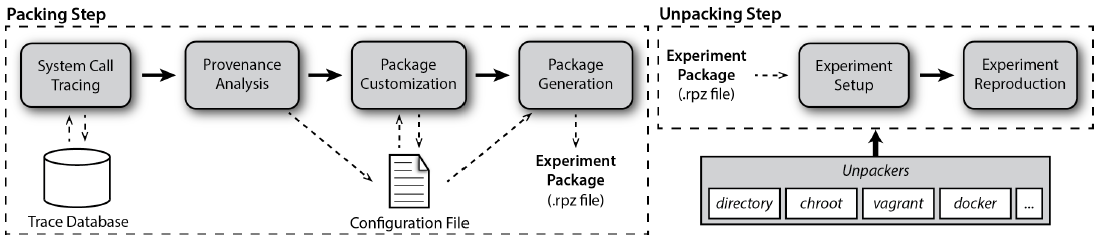
\includegraphics[width=\textwidth]{reprozip}
	\caption{Overview of the ReproZip concept from \cite{29c5846926a4497d95f276604cb0368c} }
	\label{fig:reprozip} % \label has to be placed AFTER \caption (or \subcaption) to produce correct cross-references.
\end{figure}

\subsection{Docker / Smartcontainer}\label{Smartcontainer}
Docker containers are ubiquitous in geoscience executions. The advantages of reproducible research and cost savings by using Docker containers are discussed in \cite{rs9030290} for the \gls{geobia}. The docker implementation of the image analysis was implemented with a docker image, including a user interface that can be used by non-experts. There are experiments for the more general \gls{obia} with Docker containers presented in \cite{proceedings456}. The conclusion of the previously mentioned paper is definite, with only little shortcomings in the usability. The two papers mentioned above are using the docker images to make it easy to re-run an experiment on the OBIA system. The remaining question is how the docker configuration can be preserved in a manner so that it can be reproduced in different environments. The aim of \cite{emsley2017a} is to answer this question by introducing, in addition to the Docker description file, a workflow record saving the environment and entities involved. A SPARQL query got introduced to create the possibility to use the container as a repository of data.\\ 
Another approach of preserving a docker container is a smart container introduced in \cite{Huo2015SmartCA}. The aim of a smart container is an ontology and software to preserve docker data. It uses the PROV-O standard to define the provenance. 
Docker containers are used at the EODC backend for running all services. Therefore they are part of the solution. The description files of the used docker containers are persisted in the GitHub repository of the EODC backend. Hence they are identifiable by the backend version defined in Section \ref{Design}.   


\subsection{Version Control Systems}\label{Version Control Systems}
\gls{vcs} became an essential part of all computational sciences. It enables to persist versions of code and the possibility to head back to a particular version of it. Before that, programmers tend to have multiple directories to version the code. The basic idea of VCS is that via a command line interface it is possible to set a version of the current state of the code. These versions can be accessed in the future, without changing other versions of the code and without multiple folders \cite{10.1109/MCSE.2009.194}. 
In this thesis, Gitorious (Git) is used as the version control system. Versions in Git are defined as commits and are stored locally, but can be published to an external server, where, depending on the user rights, they are accessible for other users. The commits are stored locally and remotely \cite{QuickGit}. For example, openEO uses Git as a code version tool, and GitHub is used as the publicly available server. Since openEO is an open source project, the code of every backend, core API and the client is available at GitHub. 

\subsection{Hash}\label{Hash}
Hash functions are used to validate the data without having to save the whole data. They have three important properties to work correctly. First, the probability that two different inputs have the same hash outcome has to be low. Second, it needs to be hard to find a message with the same hash value as an already known message. The properties described above makes the hash functionality a standard tool to identify data without having to save the original one \cite{3b412889270f46f59740fbf1ca8cd7e0}.  
There are different hash functions available. In this thesis, the \gls{sha}-256 is used for the data of the context model, mostly to compare differences in data outcomes.

%\begin{figure}[h]
%	\centering
%	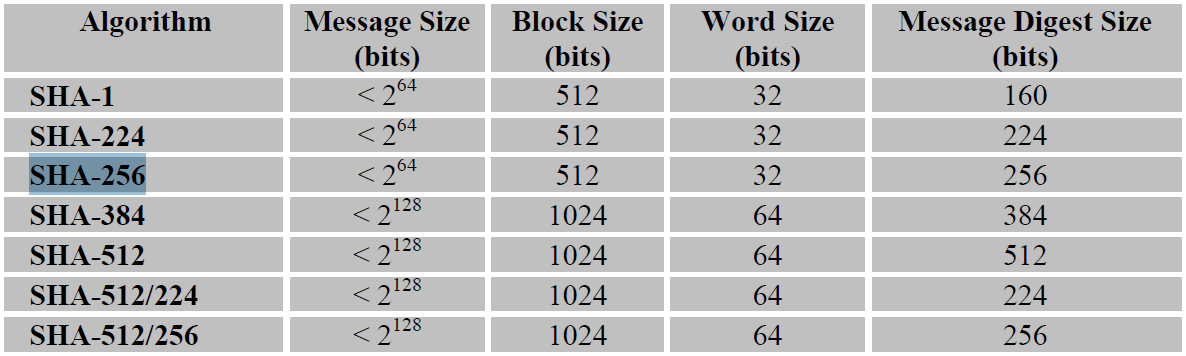
\includegraphics[width=\textwidth]{sha}
%	\caption{\cite{shapaper}}
%	\label{fig:sha} % \label has to be placed AFTER \caption (or %\subcaption) to produce correct cross-references.
%\end{figure}
%The SHA-256 is chosen in the implementation, because of the best combination of performance and security of the above described properties of the hash. 

\section{openEO}\label{openEO}
The openEO project consists of three modules, the client module written in the programming language of the users, the backend drivers that enables for every backend to understand the calls from the clients and the core API that specifies how the communication takes place. The core API is a standard that the backend providers accepted to implement on their systems. The backend drivers are the translation of the client calls to the backend specific API. This architecture decouples the clients from the backends so that every client can connect to every backend that complies with the openEO core API standard see Figure \ref{fig:api2}. An example of a workflow would be the example defined in Section \ref{example} that a scientist wants to run on the EODC backend and defines the processing with the python client in python code \cite{openeo}. 

\begin{figure}[h]
	\centering
	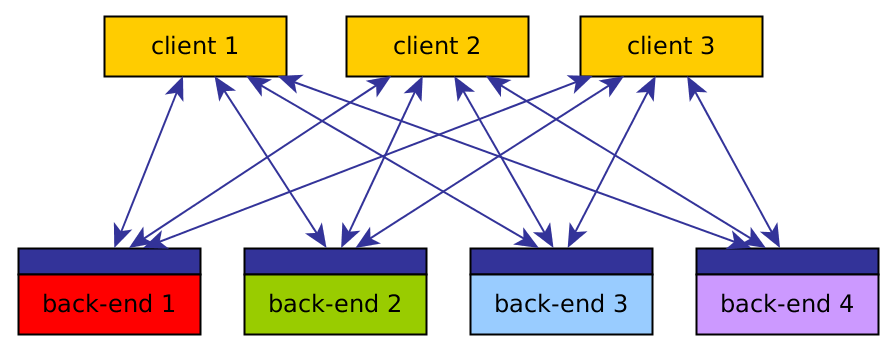
\includegraphics[width=\textwidth]{api2}
	\caption{Overview of the openEO architecture}
	\label{fig:api2} % \label has to be placed AFTER \caption (or \subcaption) to produce correct cross-references.
\end{figure}


The communication is specified as an OpenAPI description, which is a way of defining \gls{rest}ful communication in a standardized way. The definition consists of the endpoints at the backend and the requests and the responses. The whole communication protocol is specified with OpenAPI \cite{openapi}. 
In the following, the relevant RESTful request types in openEO and the policy of choosing between them are introduced.

\begin{itemize}
	\item \textbf{GET Request} \\
	GET requests are used to retrieve data and data from the backends. The functionality is limited to read operations on the data records. \\(e.g. GET /collections returns a list of available collections at the backend.)
	\item \textbf{POST Request} \\ 
	POST requests are used to create new data and data records at the backend. It is also used to carry information to the backend.  \\(e.g. POST /jobs creates a new processing job at the backend, which is defined in the body of the request.)  
	\item \textbf{PATCH Request} \\
	PATCH requests are used to update an existing record at the backend. \\(e.g. /PATCH /job/{job\_id} modifies an existing job at the backend but maintains the identifier.)
	\item \textbf{DELETE Request} \\ 
	DELETE requests are used to remove existing records from the backend. \\(e.g. /DELETE /job/{job\_id} removes an existing job from the backend.)
\end{itemize}

\subsection{Job Execution}\label{Job Execution}
The job execution workflow in openEO starts at a client application that lets the user define what has to be processed in the client-specific programming language.
The main part of the job execution definition is based on the description of what input data shall be used, which filters have to be applied, and the processes that should be executed on the data. Therefore, openEO introduces the process graph, which is defined as a tree structure describing the processes with their data and the input data identifier. The input data id is backend specific. The process graph has a \gls{json} format and gets generated by the clients in the background without users noticing it directly. In Figure \ref{fig:process_graph} there is an example of a process graph.  

\begin{figure}[h]
	\centering
	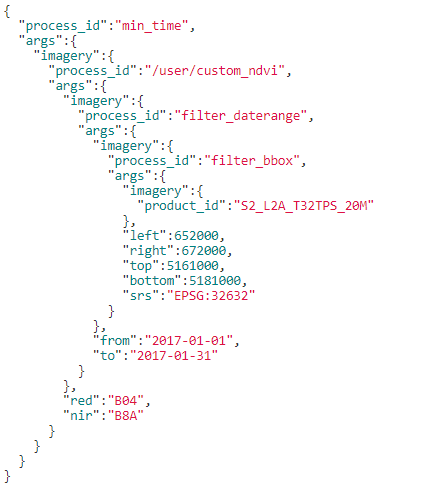
\includegraphics[scale=1]{process_graph}
	\caption{Process graph of the running example defined in Section \ref{example}}
	\label{fig:process_graph} % \label has to be placed AFTER \caption (or \subcaption) to produce correct cross-references.
\end{figure}

The backends interpret the process graph from inside out. Figure \ref{fig:process_graph} displays the process graph of the running example of Section \ref{example}. It described the calculation of the minimum NDVI image of the Sentinel 2 satellite over South Tyrol in May 2017. The element in the center of the process graph defines the input data identifier in the "imagery" block, with the "get\_collection" process id. In this case, the "s2a\_prd\_msil1c" is chosen as input data identifier, because it is the identifier for Sentinel 2 at the EODC backend.
After reading the input data id, the backend iterates one step up in the hierarchy of the process graph and calls the process "filter\_bbox" with the parameters "left", "right" and so on, which is responsible for filtering the image spatial (e.g. the area over South Tyrol). After that, the "filter\_daterange" process is used to only take imageries from May 2017. Every process beginning with "filter\_" is a filter operation that specifies the selection of the input data. The output data of the previous process is the input data of the next process. After the last filtering process, the NDVI gets called by "NDVI" with the parameters "red" and "nir", which take the identifier of the bands of near-infrared and red light, which is needed by the NDVI process (see Section \ref{example}). After that, the minimum value is taken from all images using the "min\_time" process, which then results in a single image. In Figure \ref{fig:process_graph_diagram}, the same process graph is visualized from the backend point of view, visualizing the order of how it gets executed. To transfer the process graph in Figure \ref{fig:process_graph} at a backend, it gets sent in the body of the POST /jobs endpoint request.

\begin{figure}[h]
	\centering
	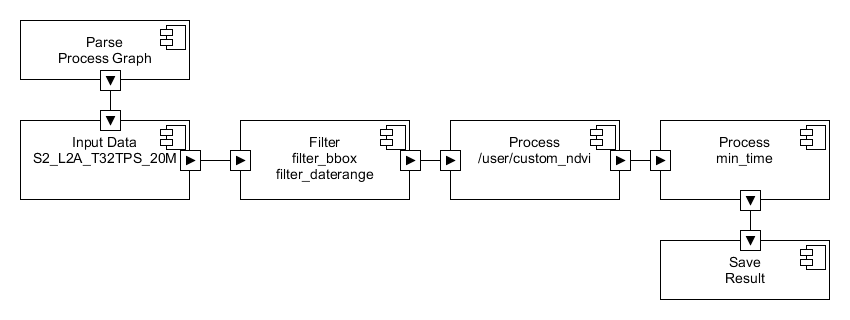
\includegraphics[width=\textwidth]{backend_pg}
	\caption{Action chain of the backend after receiving the process graph of Figure \ref{fig:process_graph}}
	\label{fig:process_graph_diagram} % \label has to be placed AFTER \caption (or \subcaption) to produce correct cross-references.
\end{figure}

There are two different kinds of process executions depending on the capabilities of the backend, synchronous and asynchronous calls. Synchronous calls are directly executed after the backend receives them, and the user has to wait until the job is finished. For example, on the python client, the program waits after sending the process graph to the backend until the backend returns the result, which is directly returned to the user. An asynchronous call does not get executed until the user starts the execution on the backend through an additional endpoint call. When the processing is finished, the user can download the result at another endpoint of the backend. For asynchronous calls, there is the possibility to subscribe to a notification system on the backend, so that the user gets notified when the job execution finished.     
The processes are defined at the openEO core API and therefore independent of the backend they get called at, other than the data identifier, which is different for every backend.  
\\
The previous example uses a process graph that only consists of the available processes and data of the backend. Within the openEO\footnote{https://github.com/Open-EO/openeo-openshift-driver/tree/release-0.0.2} project, there is the possibility to define individual processes and execute them on the backend. In the project, they are called “user defined functions” and are at the writing of this thesis still not well-defined but are code written by the openEO user that gets sent to the backend and executed there at a secure environment. The user can define processes and can run them with the data provided at the backend, using the infrastructure of the backend. Every backend has to define what the restrictions on user defined functions are. 

\subsection{Backend Overview}\label{Backend Overview}
Even though the backends implement the openEO core API standard, they are still diverse behind this abstraction layer. Some backends have already an API, where the openEO calls have to be adapted to. There are 7 partners within the openEO project that are implementing a backend driver. The backends have to manage the translation of the process graph to the actual code that executes the defined process chain. The billing of the users can be completely different on every backend. In Table \ref{Tab:backends} there is an overview of all contributing openEO backends and the related GitHub repository.
\begin{table}[]
	\caption{List of all backend providers of the openEO project}
	\begin{tabular}{l|l}
		\textbf{Organisation} & \textbf{GitHub}  \\ \hline
		EODC & \url{https://github.com/Open-EO/openeo-openshift-driver} \\ \hline 
		VITO & \url{https://github.com/Open-EO/openeo-geopyspark-driver} \\ \hline  
		Google  & \url{https://github.com/Open-EO/openeo-earthengine-driver} \\ \hline  
		Mundialis & \url{https://github.com/Open-EO/openeo-grassgis-driver} \\ \hline 
		JRC & \url{https://github.com/Open-EO/openeo-jeodpp-driver} \\ \hline
		WWU & \url{https://github.com/Open-EO/openeo-r-backend} \\ \hline
		Sinergise & \url{https://github.com/Open-EO/openeo-sentinelhub-driver} \\ \hline
		EURAC & \url{https://github.com/Open-EO/openeo-wcps-driver} \\ 
	\end{tabular}
	\label{Tab:backends}
\end{table}

\subsection{EODC Backend}\label{EODC Back End}

The EODC backend is one of the contributing backend providers of the openEO project. It is, in general, a python implemented backend that uses virtualization technologies for job execution. The overlaying technology is OpenShift (using Kubernetes) \footnote{https://www.openshift.com/learn/what-is-openshift/}, which is capable of scaling Docker containers and handles the execution of them. In the docker containers, the python code for the processing gets executed. The docker description files and the python code is available on GitHub. In this thesis, the latest version of the EODC backend provided in GitHub with the version 0.3.1 is used. In this version, every process of the openEO process graph is represented by an own Docker container running the python code needed. The python library Flask accomplishes the service layer for accessing the backend. EODC provides only data from Sentinel 2 and Sentinel 1 within the openEO project. The provided data are satellite images from the European Space Agency (ESA), which gets the raw data coming directly from the Sentinel satellites. \\
The data management of EODC is file-based, so every image data is stored in a different directory and filename combination. Data is provided via PostgreSQL database including the PostGIS\footnote{https://postgis.net} plug-in. The provided query tool for EODC users is the \gls{ogc} standard interface\gls{csw}\footnote{http://cite.opengeospatial.org/pub/cite/files/edu/cat/text/main.html}. In Figure \ref{fig:eodceer}, an overview of the EODC database is displayed. The structure is retrieved from the GitHub repository of the EODC backend\footnote{https://github.com/Open-EO/openeo-openshift-driver}, where every database entity is defined. Every Process entity can have parameters described by the Parameter entity. The process node is representing one node in a process graph and is therefore related to exactly one ProcessGraph entity. Every Job has a related process graph, there may be jobs that use the same process graph, but in the current set up they are persisted both in the database.

\begin{figure}[h]
	\centering
	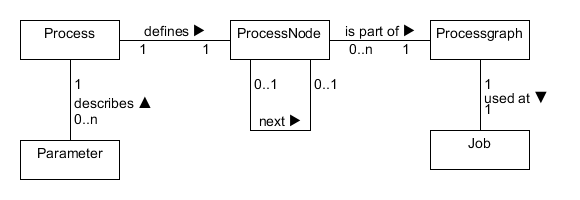
\includegraphics[width=\textwidth]{eodc_eer}
	\caption{Overview of the EODC database structure.}
	\label{fig:eodceer} % \label has to be placed AFTER \caption (or \subcaption) to produce correct cross-references.
\end{figure}

\section{Summary}

For the research areas that are related to the solution of the thesis, a vast amount of literature is available. The problem description of the thesis has many possible solutions described in this chapter. The outcome of this thesis has the aim of making it easy for the scientists to reproduce experiments, other than presented solutions for earth observation science like the VZJ approach or the GPF, which tries to motivate scientists to do it themselves. The implementation of Section \ref{Implementation} builds on existing systems like the implementation of the CCCA query store. The following chapter describes the design of the solution. 

 
\chapter{Design}\label{Design}

\todo{Gesamte Thesis: Present simple \& Past simple and not "could / would" So: we have implemented --> we implemented}
\todo{Gesamte Thesis: Restructure passive sentences}
\todo{Gesamte Thesis:Konsistente Verwendung von Begriffen --> Glossary ?? --> workflow (Beschreibung des Experiments aus sicht des wissenschaftlers), job (Definition des im backend durchgeführten parts), workflow, process graph (technische Beschreibung bzw. Definition des jobs)}
\todo{Gesamte Thesis: Wortwiederholungen sind gut !!}
\todo{Gesamte Thesis: Unnötige Wörter / Sätze weg z.b. briefly, some, also, ...}
\todo{Gesamte Thesis: Kurze einfache Sätze}
\todo{Gesamte Thesis: Eher Reproducibility schreiben in den Allgemeinen Kapiteln, aber in den RQ repeatability schreiben}
\todo{Gesamte Thesis: Software --> Environment / Code ? --> just check correct usage}

This chapter describes the concept of capturing the environment of a geoscientific experiment. This chapter aims to explain the general concept of how to gain reproducibility in an earth observation environment. It is structured in six parts. The first part presents an overview of the concept. The next three sections describe the main components of the overview in detail, first the data identification part, then the backend provenance and the job dependent provenance. The following section defines the resulting context model. The next section of this chapter defines the user services needed to use the data of the context model from an earth observation scientist's perspective. Section \ref{Design:User Defined Functions} gives an overview of the capturing of \gls{udf}. The following Chapter \ref{Implementation}, shows an implementation of the concept of this chapter at the EODC backend. 



\section{Overview}\label{Design:Overview}
This section presents an overview of the concept, and Figure \ref{fig:overview} visualizes it. The white boxes represent the components that every backend driver has in place. The green elements in Figure \ref{fig:overview} are the proposed extensions of this design. The following steps describe the typical job execution workflow:

\begin{figure}[h]
	\centering
	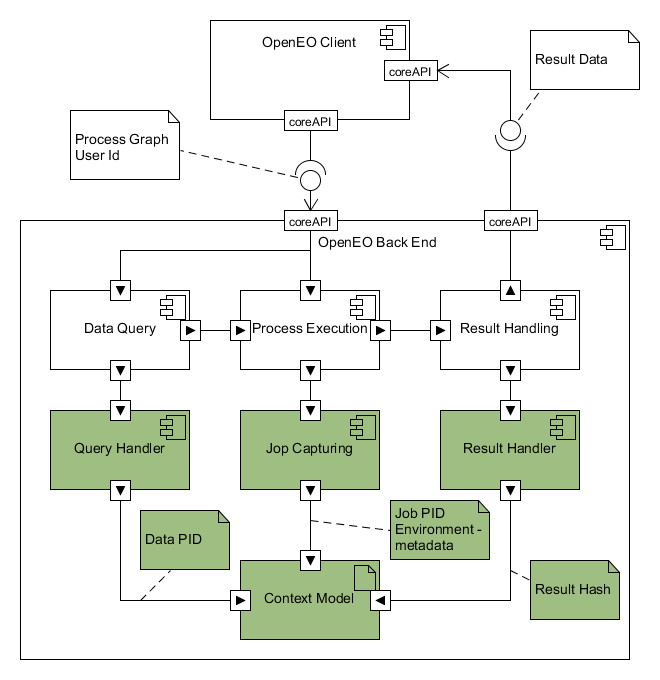
\includegraphics[scale=0.6]{design_overview}
	\caption{Overview of the Design}
	\label{fig:overview} 
\end{figure}

 \begin{enumerate}
	\item \textbf{\gls{eo} Client} \\
	The user defines the input data, the filter operations, and the processes that need to be executed at the backend via an earth observation client. Then the user orders the job to be executed. Therefore the client creates a process graph description. The backend driver interface (e.g. openEO) sends the user identification and the process graph via a RESTful endpoint.    
	\item \textbf{Data Query} \\ 
	The \textit{Data Query} component receives the process graph and parses the data identifier and the filter operations out of it to query for the input data records needed for the job. The \textit{Data Query} forwards these to the \textit{Process Execution} component.
	\item \textbf{Process Execution} \\
	The \textit{Process Execution} component receives the process graph and the input data from the \textit{Data Query} component. It parses the processes from the process graph and executes them in the order of appearance. After every process defined in the process graph got executed, the \textit{Process Execution} component forwards the resulting data to the \textit{Result Handling} component.   
	\item \textbf{Result Handling} \\ 
	The \textit{Result Handling} component receives the results from the \textit{Process Execution} component and persists all data about the job and the result. In the meantime, the resulting data is sent back to the client application if the job is not a batch job. If it is a batch job, the user has to order the results from the backend actively.  
\end{enumerate}

Every single component has to be identifiable, to make the whole workflow reproducible. Hence, the following elements get introduced as additional components to the backend.

 \begin{itemize}
	\item \textbf{Query Handler} \\
	The \textit{Query Handler} component is responsible for applying data identification to the backend. The query has to be persisted and the resulting data generated by the \textit{Data Query} component has to be identifiable by a PID. Section \ref{Design:Data Identification} describes the \textit{Query Handler} in more detail.     
	\item \textbf{Job Capturing} \\ 
	The \textit{Job Capturing} component is responsible for enabling code identification of the used software at the backend. Therefore, a PID of the code used for the processing has to be introduced. In addition, data of the job execution environment gets captured, to gain feedback information for the users and capture the environment of the execution. Section \ref{Design:Job Capturing} describes the \textit{Job Capturing} component in more detail.
	\item \textbf{Result Handler} \\
	The \textit{Result Handler} component is responsible for creating a comparable result checksum or hash. The data created by an earth observation backend might be too big to be persisted, hence there need to be a checksum or hash to be capable of confirming equal results. Section \ref{Design:Result Handler} describes the \textit{Result Handler} component in more detail.   
	\item \textbf{Context Model} \\ 
	The context model is not a component, but a data set that contains all the data mention in the previous components. One context model is related to one job execution. Section \ref{Design:Context Model} provides more detailed information about the context model. 
\end{itemize}

\section{Query Handler}\label{Design:Data Identification}
The input data of the processing is crucial for the outcome of the job execution. Even though the process graph already contains an identifier of the input data, unique for the specific backend, internal changes to the data set might not result in a new identifier. So jobs called later might use another version of the input data than previous jobs. The input data has to be persisted according to the 14 steps of data provenance defined by the RDA \cite{rauber2016identification}, to prevent this. Every backend is responsible for applying data identification. It is assumed that the backends preserve the data as described in Section \ref{Data Identification}. The \textit{Query Handler} is the module where the data persistence is implemented and depends highly on the structure and architecture of the backend. Therefore, there is no standard definition for all backends in this section. In Chapter \ref{Implementation} there is a fully implemented solution at the EODC backend. The input data is represented in the context model by the following element: 

\begin{enumerate}[(a)]
\item \textbf{Input data persistent identifier} \\
	The output of the \textit{Query Handler} is the PID of the input data related to a job execution. Every job execution uses input data, which has a PID assigned to it. Therefore, the PID is added to the job dependent context model. 
\end{enumerate}

\section{Job Capturing}\label{Design:Job Capturing}
This section aims to describe the job execution capturing and a description of data that shall be captured. The data provided by the job capturing can be categorized in static and dynamic data, where static data is defined as not dependent on job properties, and dynamic data is defined as job dependent information. In the following two sections, the static data (in this thesis called backend provenance) and dynamic data (in this thesis called job dependent provenance) are further described.      

\subsection{Backend provenance}\label{Design:Backend provenance}
The scope of this part of the context model is to get the static environment where the job execution at the backend takes place. It contains the provenance data that is independent of job execution, so it does not change through job executions, regardless of how many jobs were processed. It can only change from inside of the backend by their maintainers. The earth observation community has a great variety of different backend providers with very distinct setups. The challenge of this part of the design is to make it simple and generic. Data captured in this part of the context model is not meant to be shown to the user directly because of security issues. The following data is suggested for the backend provenance:

\begin{enumerate}[(A)]
	\item \textbf{Code identification} \\
	Every earth observation backend has to provide an identifier for the code. Therefore, a version control system has to be applied to the running services. If the backend is open source, it can provide a GitHub repository where the code is stored and publicly available. This strategy aims to get other backends with similar settings to reuse the already working setups of the running backends. In this case, the information is added to the backend provenance by saving the git repository URL, the used commit identifier and local changes to the repository. If the backend is not open source, a local or secure version control repository has to be implemented to keep track of the different code versions. The code identifier is necessary to identify differences in the backend code, and the version control system enables to jump back to versions of interest.  
	\item \textbf{API version} \\
	The backend API version is the version of the interface API it currently uses. The API defines the syntax and semantics of communication. The same API calls can resolve in different results if the version of it differs from the first execution, hence the API version is persisted in the context model.
	\item \textbf{Backend version} \\
	The backend version is an identifier that gets updated on every change of the backend. It includes changes on the hardware and software so that every change on the code identifier or the API version results in a new backend version. It is essential to implement a tool to automatically capture the environment data and persist it in a separate backend version store, to provide long term stability of the capturing, . Every change on any of the described backend data has to be detected automatically and have to result in a new backend version.   
	\item \textbf{Publication timestamp} \\
	The publication timestamp describes the time when the version was accessible at the backend. The timestamp stands for the beginning of a backend version. If there exists no timestamp after that, then it is the currently used version. It enables the possibility to find the version of the backend used by a job executed in the past, by only knowing the time it was executed.    
\end{enumerate}

\subsection{Job dependent environment}\label{Design:Job dependent provenance}
This section describes the job dependent provenance of the context model. The data captured is tied to specific job execution, so for every job, a new context model gets created. The process graph is already a description of the processes that run at the backend. So sending the same process graph to the same backend again shall result in the same outcome. To assure that the process graph can be re-executed in the same way as the original execution, data about the first execution gets captured. 
The following subsections describe the single elements of the context model in more detail. 

\subsubsection{Backend provenance}\label{Job:Backend provenance}
The backend provenance described in Section \ref{Design:Backend provenance} defines the version of the code that is executed and therefore, has to be added to the job context model. Over time the backend provenance gets updated so that every job need to persist a reference to the original backend version at the execution time. There are two solutions to achieve this. First, the identifier of a specific version of the backend gets added to the context model. In this case, the data of the backend environment versions have to be persisted and accessible. The other solution is to put a timestamp of the execution into the job execution context model.

\begin{enumerate}[(b)]
	\item \textbf{Backend provenance / code identifier} \\
	The backend provenance represents the version of the backend provenance during the job execution. Since for every change on the backend, a new version is applied, the version of the backend is used as a code identifier for the execution. Another solution is to persist an execution timestamp so that the version of the given time can be identified.
\end{enumerate}

\subsubsection{Process Environment}\label{Job:Process Data}
This section describes the capturing of the process itself. As mentioned above, the incoming process graph describes the process, but to be sure that the same process id results in the same code, the code version has to be added to the context model. To be able to identify code from different versions, source control management needs to be installed. An example of doing so is persisting the backend source code on a public platform like GitHub. The entry in the context model related to this was mentioned in Section \ref{Design:Backend provenance}.  \\
The way of executing a specific process graph is not only related to the code running it, but also by the dependencies of the code. Therefore, the programming language version and the additional used libraries of it are persisted in the context model. To gain meta-information about the processing the start time and end time can be added to the context model via timestamps. It leads to the following capturing elements in the job context model.

\begin{enumerate}[(a)]
	\setcounter{enumi}{2}
	\item \textbf{Programming language}\\
	The programming language of the code that is used for the processing. Besides, the version of the programming language has to be included in this information.
	\item \textbf{Dependencies of the programming language}\\
	The dependencies of the programming language shall be captured and added to the context model to identify the environment of the code execution. The version of the packages have a high influence on the outcome, hence can be included in the context model. For example, in python, the installed modules are added with their versions to the context model. The information stored in this element is related to the job execution, because it depends on the workflow of the execution, how the environment is configured, since the job execution may be done in a dynamically generated container.
	\item \textbf{Start and end time of process execution}\\
	On the beginning of the process execution and at the end of it, a timestamp is created. The context model persists these timestamps.
\end{enumerate}

\section{Result Handler}\label{Design:Result Handler}
The output data of the processing has to be captured as well to be able to compare job execution outcomes. In earth observation tasks, the results can be rather significant, that is why a single generated hash value of the output result is enough. The output data does not have to be identifiable within the scope of this thesis, but just checkable of identity with other executions. Therefore, a generated hash value of the output data is sufficient. The aim of the output data capturing is not to add the possibility to find differences between results but to be able to see that the results are different. Even though the input data of typical earth observation experiments are significant, the output of such experiments are images of various sizes.   

\begin{enumerate}[(f)]
	\item \textbf{Result hash} \\
	The output result of the job need to be verifiable and therefore, need to be persisted. An easy way to achieve this is to take the hash value over the output files sorted by the alphabetical ascending filenames.
\end{enumerate}

 
\section{Context Model}\label{Design:Context Model}

The context model is the data record that saves the provenance of job execution.  The backend provider infrastructure defines the type of storage it is persisted. It can e.g. be stored in a relational database or a file-based system as a file. It has to be integrated into the database of the backend. The backend has to store two different types of datasets. Figure \ref{fig:design_contextmodel} shows an overview of the elements of the backend used to run a job. Besides, it shows how the context model elements are used to identify the components of the backend.

\begin{figure}[h]
	\centering
	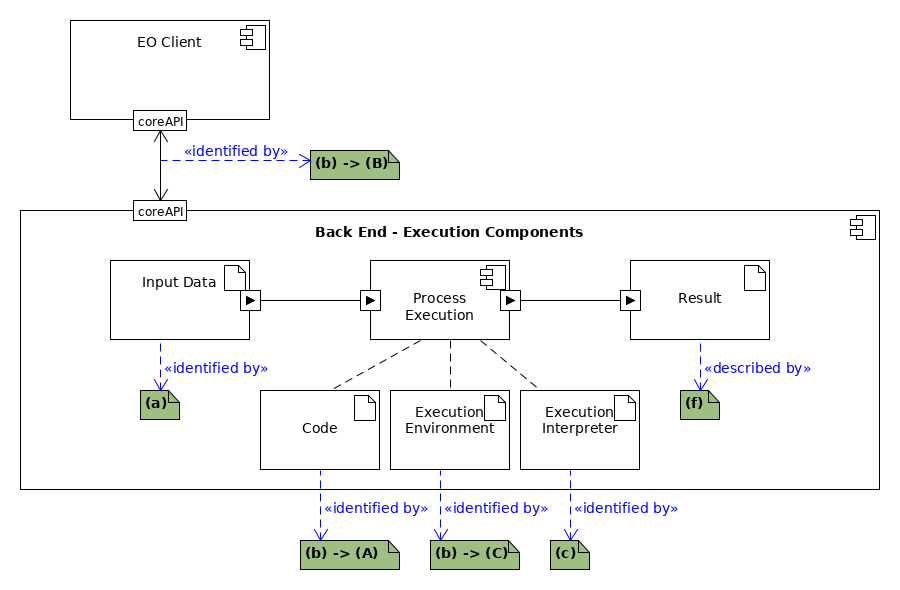
\includegraphics[width=\textwidth]{design_context_model}
	\caption{Overview of the backend execution components and the context model elements that identifies them.}
	\label{fig:design_contextmodel} 
\end{figure}

The backend environment dataset that saves job independent provenance and results in a backend version. The necessary element of the backend environment is the backend version that defines the state of the backend in a specific time. The backend version needs to be resolvable by a specific code version that was present in a past execution. Besides, data about the backend can be added. The elements ((A) - (D)) defined in Section \ref{Design:Backend provenance} are the suggestions of elements in the backend environment record. The following list recaps all of the backend environment elements: 

\begin{enumerate}[(A)]
	\item \textbf{Code identification} \\
	Enables the identification of the code of a backend version.
	\item \textbf{API version} \\
	Enables the identification of the API version of a backend version.
	\item \textbf{Backend version} \\ 
	Identifies the whole backend.
	\item \textbf{Publication timestamp} \\ 
	Enables the identification of a backend version at a specific time.
\end{enumerate}

The job execution context model that includes all information that is dedicated to a specific job is persisted in the context model. There are three necessary elements in the job context model. The input data identifier has to be persisted in the context model so that it can be identified and used in future job executions. The used version of the backend related to the execution has to be included in the context model, to be able to re-execute it with the same code in the future. The output hash has to be added to the job dependent context model so that different results can be detected. The following list recaps the elements of the job context model described in Section \ref{Design:Job dependent provenance}: 

\begin{enumerate}[(a)]
	\item \textbf{Input data persistent identifier} \\
	Identifies the input data of the job.
	\item \textbf{Backend provenance / code identifier} \\
	Identifies the backend version (C) during the execution of the job. Connects the job context model with the backend environment dataset.
	\item \textbf{Programming language} \\
	Identifies the programming language and version used by the job.
	\item \textbf{Dependencies of the programming language} \\
	Identifies the dependencies of the programming language used by the job.
	\item \textbf{Start and end time of process execution} \\
	Provides the start and end time of the job execution.
	\item \textbf{Result hash} \\
	Describes the job results for comparing it with other job results.
\end{enumerate}

\section{User Services}\label{Design:User Interface}

This section describes the information for the users and how it is provided. The capturing described in the previous sections consists of information about the backends that shall not be passed entirely to the users in detail. For example, it is maybe a security risk to provide information on specific programming language packages. On the other hand, the users need to be able to see the differences in job executions and get environment information about the backends. Therefore, there has to be a filter on which data cannot be shown to the users. Every captured information is not necessarily useful for users. Data that is not secure to the user has to be defined by the different backends themselves. The earth observation community has a very diverse set of backends, and everyone has a unique company security guideline.\\ 
Provenance information need be provided to the user. Therefore, there have to be additions to the core API specification. Additional endpoints for the users to get information about the backend have to be created for the core API, backend, and client. The following recommendations are for backend and client provider to make features related to the context model accessible for the users.

\begin{enumerate}[I.]
\item \textbf{Backend version} \\
	There has to be an endpoint for users to retrieve backend specific information, especially the current version. The aim of it is to present the users with information about the current state of the backend and to help users to decide, which backend they want to use. 

\item \textbf{Detailed Job Information} \\
	The backend has to provide an endpoint to retrieve information about an already executed job. The provenance of the job has to be presented in there. At least the resolvable persisted identifier of the input data, the backend version, and the result set hash has to be added to the view. In addition to this, the whole data of the context model can be made accessible. The resolvable identifier URL of the input data and the GitHub information can be provided, to make it more transparent for users.   

\item \textbf{Comparing Two Jobs} \\
	The API has to add an endpoint for providing a comparison of two different jobs.  Every item of both of the context models of both jobs has to be compared if they are equal or not. Therefore, the response of the comparison request consists of the differences in the context model between two jobs.

\item \textbf{Data Identifier Landing Page} \\
	After the job is executed, the input data has a relating input data PID. The PID has to be resolved by a landing page. The landing page provides the user with information about the input dataset, and the query gets re-executed to view the actual input data files upon request and given sufficient permissions.
    
\item \textbf{Re-use of Input Data} \\
	The backend has to provide an endpoint to the user to re-use specific input data in another job. Therefore, the API allows to include the use of an input data PID in the process graph, so that users can include cited data directly in a newly created job description.   
\end{enumerate}

\section{User Defined Functions}\label{Design:User Defined Functions}
This section describes a possible capturing method of User Defined Functions (UDF). UDFs are customized code written by the user that gets executed in a virtualization environment at the backend provider. In theory, the user defines a docker base image and the code that should run in it. It is a black box for the backend provider since they can not know what processes run in the docker container. Therefore, the capturing concept needs to be different than the typical way of executing jobs at the backend. The code and the docker base image has to be persisted by the backend provider. Besides, the timestamp of the execution, to be able to identify the backend version at the execution. This is a rather new concept in earth observation science and not implemented in the EODC backend, hence the implementation of the capturing is not part of this thesis.

\section{Summary}
This chapter presented the concept of the proposed solution system. The data elements needed to be able to reproduce a job execution are presented and described. The data identification has to be implemented according to the RDA recommendations, to achieve it. The backend provenance got defined by the identification of the software and the version of the backend. The job dependent environment describes the environment of the job execution information and the resulting hash. The data of the job execution got summarized in the context model. It consists of the data needed to answer the research questions of Chapter \ref{Introduction}. In addition to the data description, the needed user services to provide the functionality for the users got described in the last chapter. The next chapter presents the implementation of the design of this chapter at the EODC backend.    

\chapter{Implementation}\label{Implementation}
\todo{Always "the backend" not "the EODC backend", just in the first mentioning of the section}

\todo{Gesamte Thesis: Present simple \& Past simple and not "could / would" So: we have implemented --> we implemented}
\todo{Gesamte Thesis: Restructure passive sentences}
\todo{Gesamte Thesis:Konsistente Verwendung von Begriffen --> Glossary ?? --> workflow (Beschreibung des Experiments aus sicht des wissenschaftlers), job (Definition des im backend durchgeführten parts), workflow, process graph (technische Beschreibung bzw. Definition des jobs)}
\todo{Gesamte Thesis: Wortwiederholungen sind gut !!}
\todo{Gesamte Thesis: Unnötige Wörter / Sätze weg z.b. briefly, some, also, ...}
\todo{Gesamte Thesis: Kurze einfache Sätze}
\todo{Gesamte Thesis: Eher Reproducibility schreiben in den Allgemeinen Kapiteln, aber in den RQ repeatability schreiben}
\todo{Gesamte Thesis: Software --> Environment / Code ? --> just check correct usage}

This chapter presents the EODC prototype of the concept described in Chapter \ref{Design}. The implementation consists of all suggested changes that have to be made to the openEO workflow, including parts of the backend, core API, and the client. Thus, all three parts of the openEO project architecture get modified in the presented solution. In the openEO project, there is a vast amount of backends and clients implemented in parallel, which are all compatible with each other. One of each of the clients and the backends are used for the proof of concept of this thesis. The python client\footnote{https://github.com/Open-EO/openeo-python-client} is modified for this thesis. The EODC backend\footnote{https://github.com/Open-EO/openeo-openshift-driver} gets used for the backend part. The motivation for choosing this options is that python is the most common programming language at the contributing backends of the openEO project. Both of the chosen implementations are using python as their primary programming language. The adaptations described in Chapter \ref{Design} are implemented for the usage of the python client accessing the EODC backend driver. The resulting prototype is open source and can, therefore, be used by other backend providers with a similar setup.  

The implementation is structured in four parts. The following four sections describe these parts in detail. The first section describes the data identification implementation, e.g. the implementation of the RDA recommendations at the EODC backend. Section \ref{Implementation:Backend provenance} is about the implementation of the automated backend provenance tracking tool that captures data defined in Section \ref{Design:Job Capturing}. After that Section \ref{Implementation:Job dependent provenance} is about the implementation of the job execution provenance. The last section is about the implementation of user interface additions defined in Section \ref{Design:User Interface}.     

\section{Data Identification}\label{Implementation:Data Identification}

As defined in Section \ref{Design:Data Identification}, the RDA recommendations have to be applied to every backend provider individually. This section presents the data identification solution for the EODC backend. Other openEO backend providers can use the presented approach as well to enable data identification on their backend setup. All backend providers can use some parts of the implementation. The workflow of users getting and using the data identifier, including the landing page is described in Section \ref{Implementation:User Interface}. \\

\subsection{Query Store}
The centerpiece of the RDA recommendations is the implementation of a Query Store. Queries in the Query Store must be comparable, identifiable, and persisted. At the EODC backend, the Query Store is realized with two new tables in the existing PostgreSQL database. In Figure \ref{fig:eer_rda} the EODC database structure from Figure \ref{fig:eodceer} is visualized with the proposed additional tables. The new \textit{Query} table consists of the query dataset specified by the RDA recommendations. The \textit{QueryJob} table defines the relation between Job and Query. In the current version of the openEO core API, it is only possible to have one input data query used by a job. In the future, there may be the possibility to have more than one input data query related to one job. Hence the \textit{QueryJob} table gets introduced. 

\begin{figure}[h]
	\centering
	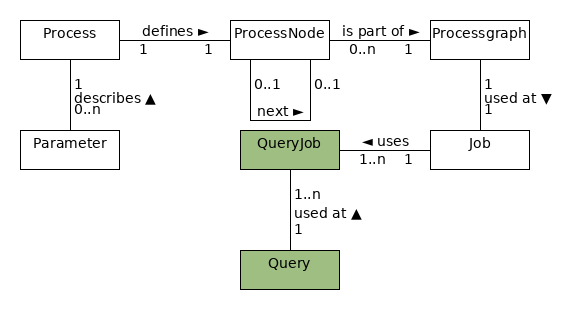
\includegraphics[width=\textwidth]{eodc_eer_rda}
	\caption{Overview of the database of EODC with the proposed additional tables (green).}
	\label{fig:eer_rda} % \label has to be placed AFTER \caption (or \subcaption) to produce correct cross-references.
\end{figure}

\subsection{Query Handler Workflow}
Figure \ref{fig:impldataid} shows an overview of the data identification solution of the EODC backend. The green parts of the diagram are representing the additions proposed in the thesis. The \textit{Query Handler} itself is an additional python module in the EODC backend that gets called after the job execution. 

\begin{figure}[h]
	\centering
	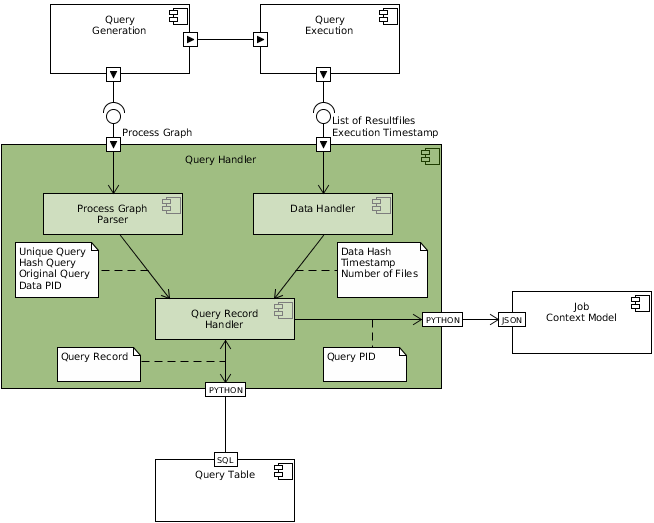
\includegraphics[width=\textwidth]{implementation_dataidentification}
	\caption{Overview of the proposed data identification workflow at the EODC backend}
	\label{fig:impldataid} % \label has to be placed AFTER \caption (or \subcaption) to produce correct cross-references.
\end{figure}

The \textit{Query Generation} and \textit{Query Execution} components of the EODC backend provide the input data of the \textit{Query Handler}. The process graph is the raw input process graph received by the backend driver from the client application. The list of result files is the result of the query execution process and therefore, the input data of the workflow. The \textit{Query Execution} component provides the execution timestamp additionally. The \textit{Query Handler} consists of the following components:

 \begin{itemize}
	\item \textbf{Query Processor} \\
	The Query Processor takes the query as input and generates the necessary query data out of it. Since the process graph at this point also includes the processes and not only the filter operations, this step is necessary. The output consists of the original query, the unique/normalized query, the hash of the normalized query, and the persisted data identifier of the query. This information is forwarded to the Query Record Handler. The mentioned resulting items are described more in detail in the section below.   
	\item \textbf{Data Handler} \\ 
	The Data Handler is responsible for creating the result data dependent query information. The output is the hash over the file list result, the execution timestamp and additional data. In this case, the Data Handler only calculates the number of files as data output. Since EODC uses the OGC standard CSW\footnote{http://cite.opengeospatial.org/pub/cite/files/edu/cat/text/main.html} to query the data, the sorting of the resulting files is predefined. The order of the files has no impact on the processing, and openEO users are not able to choose a specific sorting. Therefore the predefined CSW sorting is used for the hash production. The results of the component are forwarded to the Query Record Handler.    
	\item \textbf{Query Record Handler} \\
	The Query Record Handler communicates with the meta database from EODC to see if an identical Query already exists. The Workflow of the Query Record Handler can be viewed in Figure \ref{fig:queryhandler_activity}. If the Query Record already exists the Query Record Handler forwards the existing Query PID to the context model, otherwise a new Query PID gets created and persisted in the Query Table. The combination of the result-file hash and the normalized query hash must not have duplicates in the \textit{Query} table. On saving the Query PID in the job context model, a \textit{QueryJob} table entry gets created to store the relation between the job id and the Query PID. 
	
\end{itemize}

\begin{figure}[h]
	\centering
	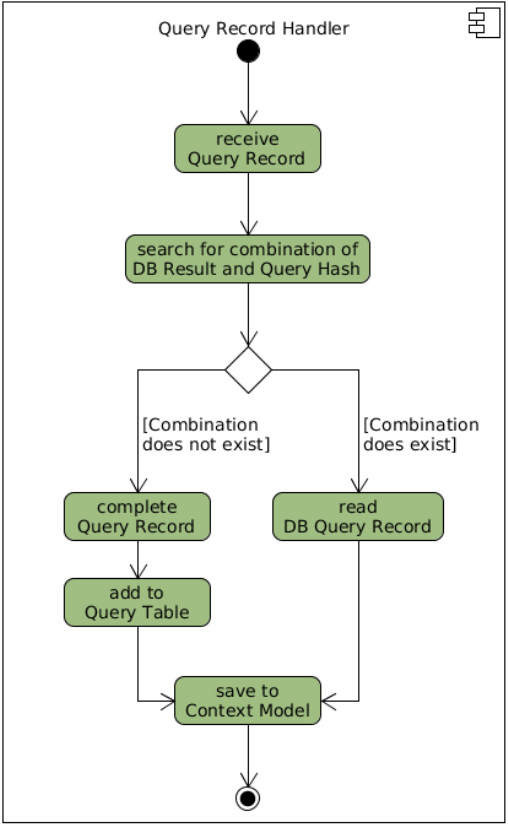
\includegraphics[scale=0.5]{queryhandler_activity}
	\caption{Activity diagram of the Query Record Handler component.}
	\label{fig:queryhandler_activity} % \label has to be placed AFTER \caption (or \subcaption) to produce correct cross-references.
\end{figure}

\subsection{Query Table Structure}

The Query Table stores the data related to the query instance, additional result, and data information. Table \ref{Tab:querytable} visualizes the Query Table structure. Example input values are used to explain how the single data entries are generated, to illustrate the Query data record. Therefore, in Figure \ref{fig:processgraph_example} there is an example input process graph.   

\begin{figure}[h]
	\centering
	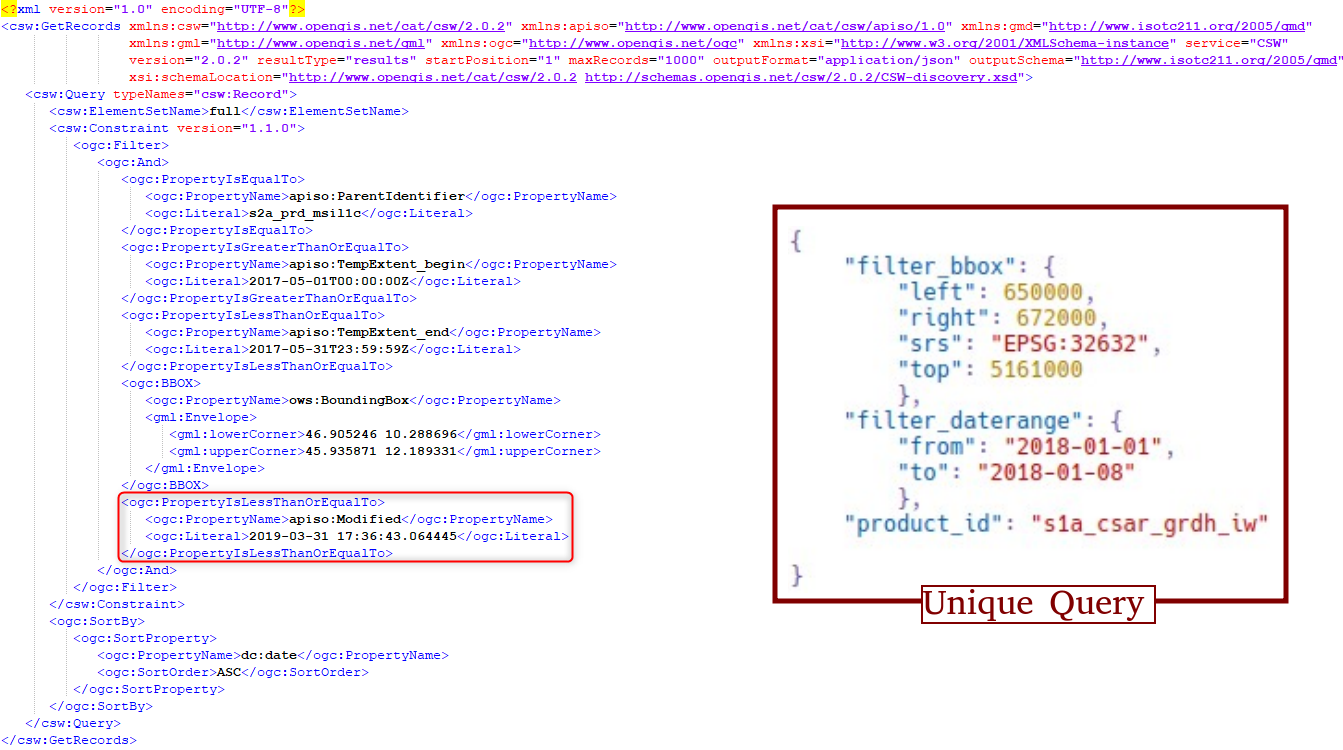
\includegraphics[width=\textwidth]{original_query}
	\caption{Example original query and unique query.}
	\label{fig:processgraph_example} % \label has to be placed AFTER \caption (or \subcaption) to produce correct cross-references.
\end{figure} 

\begin{table}[]
	\caption{Structure of the Query Table in the EODC meta database.}
	\begin{tabular}{|l|l|l|l|l|l|l|l|}
	\hline	\textbf{Query} & \textbf{Dataset} & \textbf{Original} & \textbf{Unique} & \textbf{Hash} & \textbf{Hash} &
		\textbf{Exec.} & \textbf{Add.}  \\ 
		\textbf{PID} & \textbf{PID} & \textbf{Query} & \textbf{Query} & \textbf{Query} & \textbf{Result} &
		\textbf{Timest.} & \textbf{Metad.}  \\ \hline
		\textbf{1} & \textbf{2} & \textbf{3} & \textbf{4} & \textbf{5} & \textbf{6} &
		\textbf{7} & \textbf{8} \\ \hline
		\textbf{...} & \textbf{...} & \textbf{...} & \textbf{...} & \textbf{...} & \textbf{...} & \textbf{...} & \textbf{...} \\ \hline
	\end{tabular}
	\label{Tab:querytable}
\end{table}

The following list describes how the elements of the query data set record are created in more detail:

\begin{enumerate}
	\item \textbf{Query PID} \\
	The Query PID gets generated by the python library uuid\footnote{https://docs.python.org/3/library/uuid.html}. The library is used to generate unique identifiers and used in the EODC backend for generating the job ids. In the EODC backend ids have in the beginning code for the specific entity (e.g. "jb-UUID" for Job entities). That is why the id for a Query Table entry is structured like "qu-UUID". \\
	\textit{Example: "qu-16fd2706-8baf-433b-82eb-8c7fada847da"}
	\item \textbf{Dataset PID} \\
	The dataset PID is the identifier of the satellite in the process graph (e.g. the "product\_id" element). \\
	\textit{Example: "s1a\_csar\_grdh\_iw"}	    	
	\item\textbf{Original Query} \\
	The original query is the input query of from the query execution component, which got executed by it.  \\ 
	\textit{Example: See the Original Query in Figure \ref{fig:processgraph_example}}	 
	\item \textbf{Unique Query} \\
	The unique query is the restructured query that is comparable to other unique queries. Since the order of the filters makes no difference in the outcome of the query execution, the elements of the original query are alphabetically sorted by the JSON keys to get the unique query. \\
	\textit{Example: See the Unique Query in Figure \ref{fig:processgraph_example}}	  	 	
	\item \textbf{Unique Query Hash} \\ 
	Newline and space characters are removed from the unique query string. The unique query hash is the output of the SHA-256 hash function (using the python module "hashlib") with the unique query as input.  \\
	\textit{Example: "AE7EF888CDEDF8A9A371\dots"} 
	\item \textbf{Result Hash} \\
	The result hash is the output of the SHA-256 hash function (using the python module "hashlib") with the result file list as input. Before the list is applied to the hash function it is transformed to a string and the newline and white space characters are removed. \\
	\textit{Example: "565D229FCE4772869343\dots"} 
	\item \textbf{Execution Timestamp} \\
	The execution time stamp is the input parameter of the \textit{Query Handler} and is transformed to the data type needed by the data base. The timestamp is taken by the query execution handler and is part of the query execution result. To forward it to the \textit{Query Handler} it has to be read from the result object. \\
	\textit{Example: "2018-10-17 18:03:20,609"}  
	\item \textbf{Additional Data} \\
	The additional data column of the \textit{Query} table can be used by the EODC backend to store additional information about the query execution. In the implementation of this thesis, only the number of output files are persisted in the database. The column is defined as a JSON object and can be extended with additional data easily. \\
	\textit{Example: "\{ "number\_of\_files": 10\}"}    	 
\end{enumerate}


\section{Backend provenance}\label{Implementation:Backend provenance}

The backend provenance aims to persist the versions of the backend and therefore the version of the software used to execute the jobs. The following subsections explain how the, in Section \ref{Design:Backend provenance} defined, provenance data elements are read from the GitHub repository.   
\begin{enumerate}[(A)]
\item \textbf{GitHub Repository} \\
	The GitHub repository is directly used to create the services of the EODC backend. Therefore, the currently used GitHub repository information can be read via the \gls{cli} of Git. The used commit and branch are accessed directly via the Git CLI. Listing \ref{lst:impl_backendprov} shows the Git CLI calls used to get the GitHub repository information.       

\begin{code}
	\begin{minted}{bash}
	# Receiving the Git Repository URL
	git config --get remote.origin.url 
	# Receiving Branch
	git branch
	# Receiving the commit messages with the timestamps
	git log 
	\end{minted}
	\caption{Git commands used to get access the backend identification.}
	\label{lst:impl_backendprov}
\end{code}

\item \textbf{Core API Version} \\
	Backend developers manually update the openEO core API version of the EODC backend. It is in the GitHub repository of the EODC backend. 

\item \textbf{Back End Version} \\
	Since EODC takes the code for the services directly from GitHub, the Git commit identifier is used as the version of the backend.

\item \textbf{Publication Timestamp} \\
	The publication timestamp of the EODC backend is defined by the timestamp when the Git commit happened. It is persisted by GitHub and can be retrieved via the Git CLI. 
\end{enumerate}

\section{Job dependent provenance}\label{Implementation:Job dependent provenance}
The EODC backend of the release version "0.3.1" transforms the process graph into separate docker containers. For every process in the process graph, there is a Docker container running the related python code. The input of the current process is the output of the previous process. The first process docker container has the input data defined in the process graph as an input value, which is the result of the query execution. Every process saves the results in a temporary folder dedicated to the specific process execution. Every process has its temporary output directory until the whole process chain is finished. After that, the backend deletes the temporary folders, and only the result is persisted in the job directory.
The processes must provide data about the input data, the output data, and the processing itself, to achieve the job environment data capturing described in Chapter \ref{Design:Job dependent provenance}. \\ 
The implementation adds specific information of interest to the logging of the processing and reads the logging files to generate the context model. This solution modifies and extends the existing python code and is used for the evaluation of this thesis. In Figure \ref{fig:impljobcapture}, an overview of the job capturing workflow is presented. Section \ref{Implementation:Python Implementation} describes the single parts of the overview in more detail.


\subsection{Context Model Repository}\label{Implementation:Provenance Repository}
Each executed job creates a context model. If the job gets re-executed, the context model gets replaced by the new context model. Job re-execution is internally handled as a new job with the same process graph. The functionality of letting the same job be re-executed without creating a new job id is dropped from the agenda of the openEO project in version 0.3.1 (see the GitHub repository\footnote{https://open-eo.github.io/openeo-api/v/0.3.1/apireference/}). 
The context model is stored as a JSON object in the job execution database. After the job is carried out in the EODC backend the results are saved in a folder named after the unique job identifier and the data information is stored in a PostgreSQL database (see Section \ref{EODC Back End}). Jobs are saved in the \textit{Job} table of the database, and in this solution, the context model is an additional column of it. The context model JSON object gets created by the implementations described below. \\
Table \ref{Tab:contextmodel} provides the mapping between the context model elements from Section \ref{Design} and the keys of the JSON context model object of the prototype. The elements have a one to one mapping of the context model and the JSON key except for the timestamps of the execution. The execution timestamps are part of the \textit{Job} table in the EODC database. \\
Figure \ref{fig:job_context_model} shows an example context model. It consists of all elements described for the context model in the Design section. Information on the backend environment during the execution of the job is persisted in the context model. In the context model, the backend version and the execution timestamp is persisted and can be used to identify the backend provenance of the execution time. The code environment is a list of all python dependencies with their versions installed during the execution of the jobs. Besides, the python interpreter version is added to the JSON object. How the data is captured in detail is described in the sections below.    
  


 
\begin{table}[]
	\caption{Relation of context model elements and EODC JSON context model.}
	\begin{tabular}{l|l}
		\textbf{Context Model Definition} & \textbf{JSON Key} \\ \hline
		\textbf{(a): Input data persistent identifier} & input\_data \\ \hline
		\textbf{(b): Backend provenance / code identifier} & backend\_env \\ \hline
		\textbf{(c): Programming language} & interpreter \\ \hline
		\textbf{(d): Dependencies of the programming language} & code\_env \\ \hline
		\textbf{(e): Start and end time of the process execution} & start\_time, end\_time \\ \hline
		\textbf{(f): Result hash} & output\_data \\ %\hline
	%	\textbf{J7: Backend provenance} & backend\_env \\ 
	\end{tabular}
\label{Tab:contextmodel}
\end{table}

\begin{figure}[h]
	\centering
	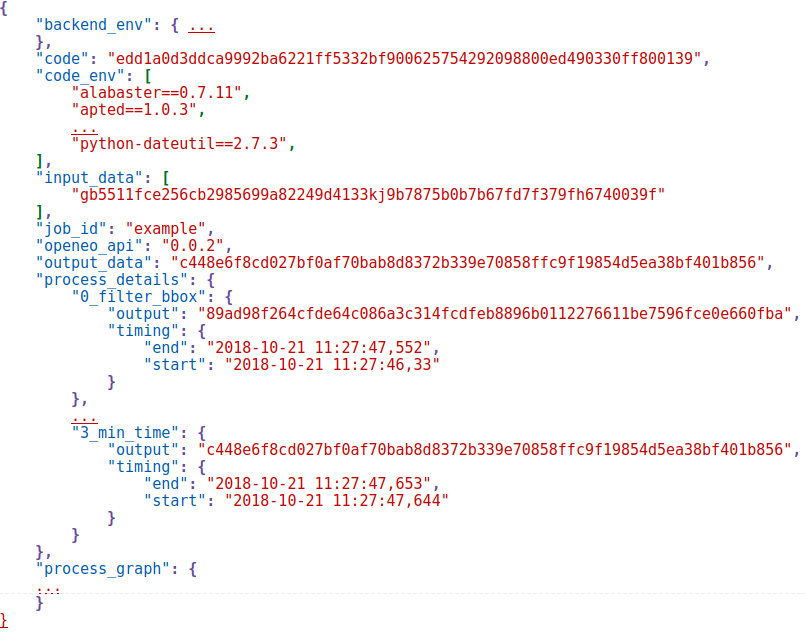
\includegraphics[width=\textwidth]{job_context_model}
	\caption{Example context model of a job execution at the EODC backend.}
	\label{fig:job_context_model} % \label has to be placed AFTER \caption (or \subcaption) to produce correct cross-references.
\end{figure}

\subsection{Python Implementation}\label{Implementation:Python Implementation}
The EODC implementation proposed by this thesis is an example for other backends, hence needs to be easy to implement and maintain. Therefore, the implementation is done in the python version of the EODC backend without any additional requirements. The python solution uses logging messages to transfer the needed data from the process execution program to the capturing tool. The cleanup service of the EODC backend driver triggers the execution of it. It is an additional python module and parses the log files after the job is finished. This solution generates, except for the additional logging calls, little impact on the existing backend implementation. The EODC backend driver has already a logging system installed. Hence the modifications are added in the existing logging policy. \\
Figure \ref{fig:impljobcapture} visualizes the additional python module \textit{Job Capturing} and \textit{Result Handler} in the context of the backend environment. The following list describes the workflow of the solution at the EODC backend driver. 

\begin{figure}[h]
	\centering
	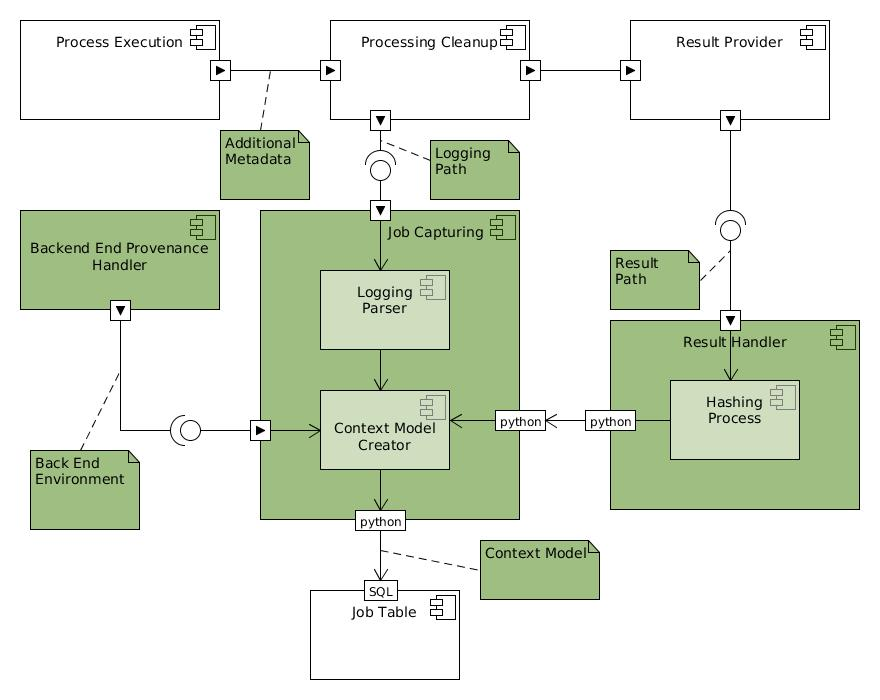
\includegraphics[width=\textwidth]{job_capturing_overview}
	\caption{Overview of the Job capturing architecture at the EODC backend}
	\label{fig:impljobcapture} % \label has to be placed AFTER \caption (or \subcaption) to produce correct cross-references.
\end{figure}

\begin{enumerate}
	\item \textbf{Process Execution} \\
	The \textit{Process Execution} module at the EODC backend is responsible for the actual execution of the job. It creates the additional logging information ((a), (c), (d) and (e) of the context model) and persists it in the logging file of the job execution. 
	\item \textbf{Processing Cleanup} \\
	After the job execution is finished, the temporary folders are deleted from the file system and the result is copied to the persisted job folder. Then the additional \textit{Job Capturing} module starts with the path to the logging file.  
	\item \textbf{Result Provider} \\
	The \textit{Result Provider} is responsible of making the result available for the user and providing the user with the feedback of the finished job. Additionally it invokes the \textit{Result Handler} module with the path of the resulting file.
	\item \textbf{Result Handler} \\
	The \textit{Result Handler} reads the result file and calculates an SHA-256 hash over it. After completion, it is provided to the \textit{Context Model Creator} module.  
	\item \textbf{Job Capturing} \\
	The \textit{Job Capturing} module parses the logging file to extract the information needed for the context model ((a), (c), (d) and (e)) and passes the formatted information to the \textit{Context Model Creator}. The \textit{Context Model Creator} needs the \textit{Result Handler} (f) and \textit{Back End Provenance Handler} (b) for the remaining parts of the context model. After receiving all necessary information the JSON context model is created and stored to the \textit{Job} table in the EODC database.    
\end{enumerate}

The following sections describe the capturing of each data element of the job dependent context model in more detail.
\begin{enumerate}[(a)]
\item \textbf{Source Input Data Identifier} \\
	The source input data identifier is the PID of the input data and query provided by the EODC query store described in Section \ref{Implementation:Data Identification}. It is forwarded to the \textit{Job Capturing} module by the \textit{Processing Cleanup} module. 

\item \textbf{Backend provenance / Code Identifier} \\
	The \textit{Job Capturing} module reads the backend provenance from the \textit{BackendMonit} output JSON file described in Section \ref{Implementation:Backend provenance}. The latest backend version during the execution is copied to the context model.

\item[(c)(d)] \textbf{Programming language and  installed packages of programming language} \\
	The \textit{Process Execution} module uses the installed python module \textit{pip} to list all installed packages including their versions. The module is at the moment used to manage the python packages of the backend. The GitHub repository of the EODC backend driver includes a python environment file to install all needed dependencies of python via \textit{pip} automatically. A feature of that tool is the \textit{pip freeze} call, which returns all installed python packages including their particular versions. It is then transformed into a JSON list object and saved to the context model. In addition to this the \textit{Process Execution} captures the python version by using the \textit{sys.version} call. All of this executions are done in the \textit{Process Execution} module, in the actual processing environment and stored in the output log file of the job execution.    

\item[(e)] \textbf{Start and end time of process execution} \\
	The start and end time of the process execution is already done at the EODC backend in the  \textit{Process Execution} module. The resulting time stamps are persisted in the \textit{Job} table of the database. The \textit{Process Execution} module adds the values to the output logging file. This solution does not add these logging entries since the EODC backend provider already implements them.

\item[(f)] \textbf{Result Identifier} \\
	The result identifier consists of the resulting data of the whole process graph execution. It is an SHA-256 hash (using the \textit{hashlib} python library) of the resulting alphabetical sorted output files, which are placed in the resulting folder of the job execution directory. In the current version of the backend, there is only one result file created, due to the limitations of the available processes.   
\end{enumerate}
\section{User Services}\label{Implementation:User Interface}
The previous sections describe only the technical insight of the backend. This section describes the implementation of the interfaces for the users. Therefore, endpoints are added to the current existing openEO core API version 0.3.1. Besides, the proposed endpoints are applied to the python client and the EODC backend. The implementation of the recommended additions of Section \ref{Design:User Interface} are described in the following:
\begin{enumerate}[I.]
\item \textbf{Backend version} \\
	Retrieving additional information about the backend was added into a new endpoint of the API. The new endpoint is a GET request called “/version” and no authentication is needed to access it. The response of the version endpoint is the whole job independent provenance information of the backend ((A)-(D), see Section \ref{Implementation:Backend provenance}). In a production version, the data may be filtered for information marked as a security risk. This endpoint is added to the EODC backend to return the latest backend version including data. The endpoint takes a timestamp as a parameter to get the backend version data of a specific time. Further additions are created to the python client so that the user can call a method in the python client called “version()” to retrieve the information of the backend directly in the python client. A result is a JSON object consisting of the backend provenance data. Listing \ref{lst:implementation_back_end_version} shows a result example.

\begin{listing}[ht]
	\begin{minted}{json}
{'branch': 'master',
'commit': '1a0cefd25c2a0fbb64a78cd9445c3c9314eaeb5b',
'url': 'https://github.com/bgoesswein/implementation_backend.git'}
	\end{minted}
	\caption{Backend version example.}
	\label{lst:implementation_back_end_version}
\end{listing}

\item \textbf{Detailed Job Information} \\
	In the openEO coreAPI, there is an endpoint to get detailed information about the job status. The endpoint path is “GET /jobs/<job\_id>” , which by the current release version of 0.3.1 only contains the execution state of the job and the job id. In addition to this, the available information of the whole job dependent provenance gets added to this endpoint in the implementation of this thesis (e.g. see Figure \ref{fig:job_context_model}). Since the python client returns the resulting JSON response from the backend as a python dictionary, there is no modification needed.

\item \textbf{Comparing two Jobs} \\
	The core API does not define the comparison of two jobs. Hence there does not exist any user interface. The modified core API defines a new endpoint in the manner of existing endpoint definitions. For this thesis, the endpoint  “POST /jobs/<job\_id>/diff” gets introduced to the new core API. In the URL of the request, the user defines the base job id, which context model is compared with other jobs. In the body of the request, the target job ids are defined in a JSON list. After getting the request from the user, the backend compares the context models of the base job with every target job occurring in the request body list. The result from the backend consists of a term for every item in the base job context model. The term “EQUAL”, if the item is the same in both context models, the difference if the items are not the same in both context models, or “MISSING” if the item is in the base job context model, but missing in the target job context model or the other way around. If an element is different, the elements that differ are visible. The latest mentioned outcome can occur if the context model definition is modified in future job executions and there are e.g. additional fields of it. The response contains the context model of all jobs with one of the previously described three states inside of the value of every item. In the python client, this feature is added with an additional function of the Job class called "diff(target\_job)". Listing \ref{lst:job_comparison} provides an example of the dictionary output of this function.

\begin{listing}[ht]
	\begin{minted}{json}
{
"process_graph":"EQUAL",
"input_data":"EQUAL",
"code_env":"EQUAL",
"output_data":"EQUAL",
"openeo_api":"EQUAL",
"different":{
   "interpreter":"Python 3.5",
   "job_id":"jb-47e062e4-d39c-4f7f-bc5e-aa877f039a84",
   "start_time":"2019-04-05 12:16:38.286217",
   "back_end_timestamp":"20190405121638.286217",
   "end_time":"2019-04-05 12:18:08.286217"}
}
	\end{minted}
	\caption{Example of resulting job comparison.}
	\label{lst:job_comparison}
\end{listing}	


\item \textbf{Data Identifier Landing Page} \\
	Depending on the backend, the input data may be restricted to the openEO interface. Therefore, the resolver of the input data PID is set within the core-API specification. In the coreAPI release version 0.3.1, there exists an endpoint to retrieve detailed information about a data set. The "GET /data/<data-pid>" endpoint is introduced. If the user calls the endpoint with a data PID, the result is the details of the underlying dataset and besides, the result of the query execution and the original query parameters. The landing page contains a link to another page with the file list after a query re-execution ("GET /data/<data-pid>/result" endpoint). If the result file list differs from the first execution, there is a list of the files that differ. Otherwise, it states that the file list is equal to the first execution. 

\item \textbf{Re-use of Input Data} \\
	To re-use the input data in different job execution, the data PID can be used in the process graph directly as source data, instead of just the unfiltered dataset identifier. If a process graph uses the input data PID, the EODC backend automatically applies the queries in the way of the first execution. It is inserted in the process "get\_collection" as an additional filter argument named "data\_pid", to pass the data PID to the process graph. Section \ref{Implementation:Use Case1} provides an example of such a process graph. If the query result data changed from the first execution of the PID, the job shall be processed nonetheless, but there has to be a warning message to notify the user.  
\end{enumerate}

\section{Use Cases}
This section shows how the use cases of Section \ref{Use Cases} can be addressed using the implementation described in the sections before. In the first section, there is an overview of how the data identification recommendations by \acrshort{rda} are implemented. 

\subsection{Use Case 1 – Re-Use of Input Data}\label{Implementation:Use Case1}
The first scenario describes the process of a researcher using openEO as a processing environment. In this use case, the focus is on the data identification and data citation part of the solution. Researchers that use openEO may want to cite the data that is used in the applied process chain. Other scientists then may want to use this data in their related research experiment. The step-by-step description of the scenario can be viewed in Section \ref{UseCase1}. In this section, the steps of the use case are executed in the evaluation environment. The implementation of the use cases is available at GitHub\footnote{https://github.com/bgoesswein/dataid\_openeo/tree/master/openeo-python-client/examples}.

\begin{enumerate}
	\item \textbf{Researcher A runs an experiment (job A) at the EODC backend.} \\
	This step is basic openEO functionality and is not influenced by the solution from the user point of view. The researcher chooses Sentinel-2 data by loading the Sentinel-2 collection of EODC with the data-set identifier "s2a\_prd\_msil1c". In the next step, the data is filtered temporally (May of 2017) and spatially (bounding box of the South Tyrol area). In the next step the researcher applies the NDVI\footnote{https://earthobservatory.nasa.gov/features/MeasuringVegetation/measuring\_vegetation\_2.php} process on the filtered data as well as the minimum value of each pixel in the time range with the "min\_time" process. The NDVI calculation needs the measurements of the satellite in near-infrared (parameter "nir") and the measurements of red light (parameter "red"). for Sentinel 2 data of the EODC the band identifiers represent the two measurements "B08" for near-infrared and "B04" for the visible red light. The last two lines create a job at the backend with the specified process graph and start the execution of it.
	At the backend the \textit{Query Handler} is generating a new data PID or returns an already existing one if the same query got executed in the past. The following python client code represents the experiment of Researcher A.
	
\begin{code}
	\begin{minted}{python}
import openeo
EODC_DRIVER_URL = "http://openeo.local.127.0.0.1.nip.io"

con = openeo.connect(EODC_DRIVER_URL)

# Choose dataset
processes = con.get_processes()
pgA = processes.get_collection(name="s2a_prd_msil1c")
pgA = processes.filter_daterange(pgA, extent=["2017-05-01", 
"2017-05-31"])
pgA = processes.filter_bbox(pgA, west=10.288696, 
south=45.935871, east=12.189331, 
north=46.905246, crs="EPSG:4326")

# Choose processes
pgA = processes.ndvi(pgA, nir="B08", red="B04")
pgA = processes.min_time(pgA)

# Create job A out of the process graph A (pgA)

jobA = con.create_job(pgA.graph)
jobA.start_job()
	\end{minted}
	\caption{Researcher A runs job A with the python client.}
	\label{lst:impl_usecase1_1}
\end{code}	

\begin{figure}[h]
	\centering
	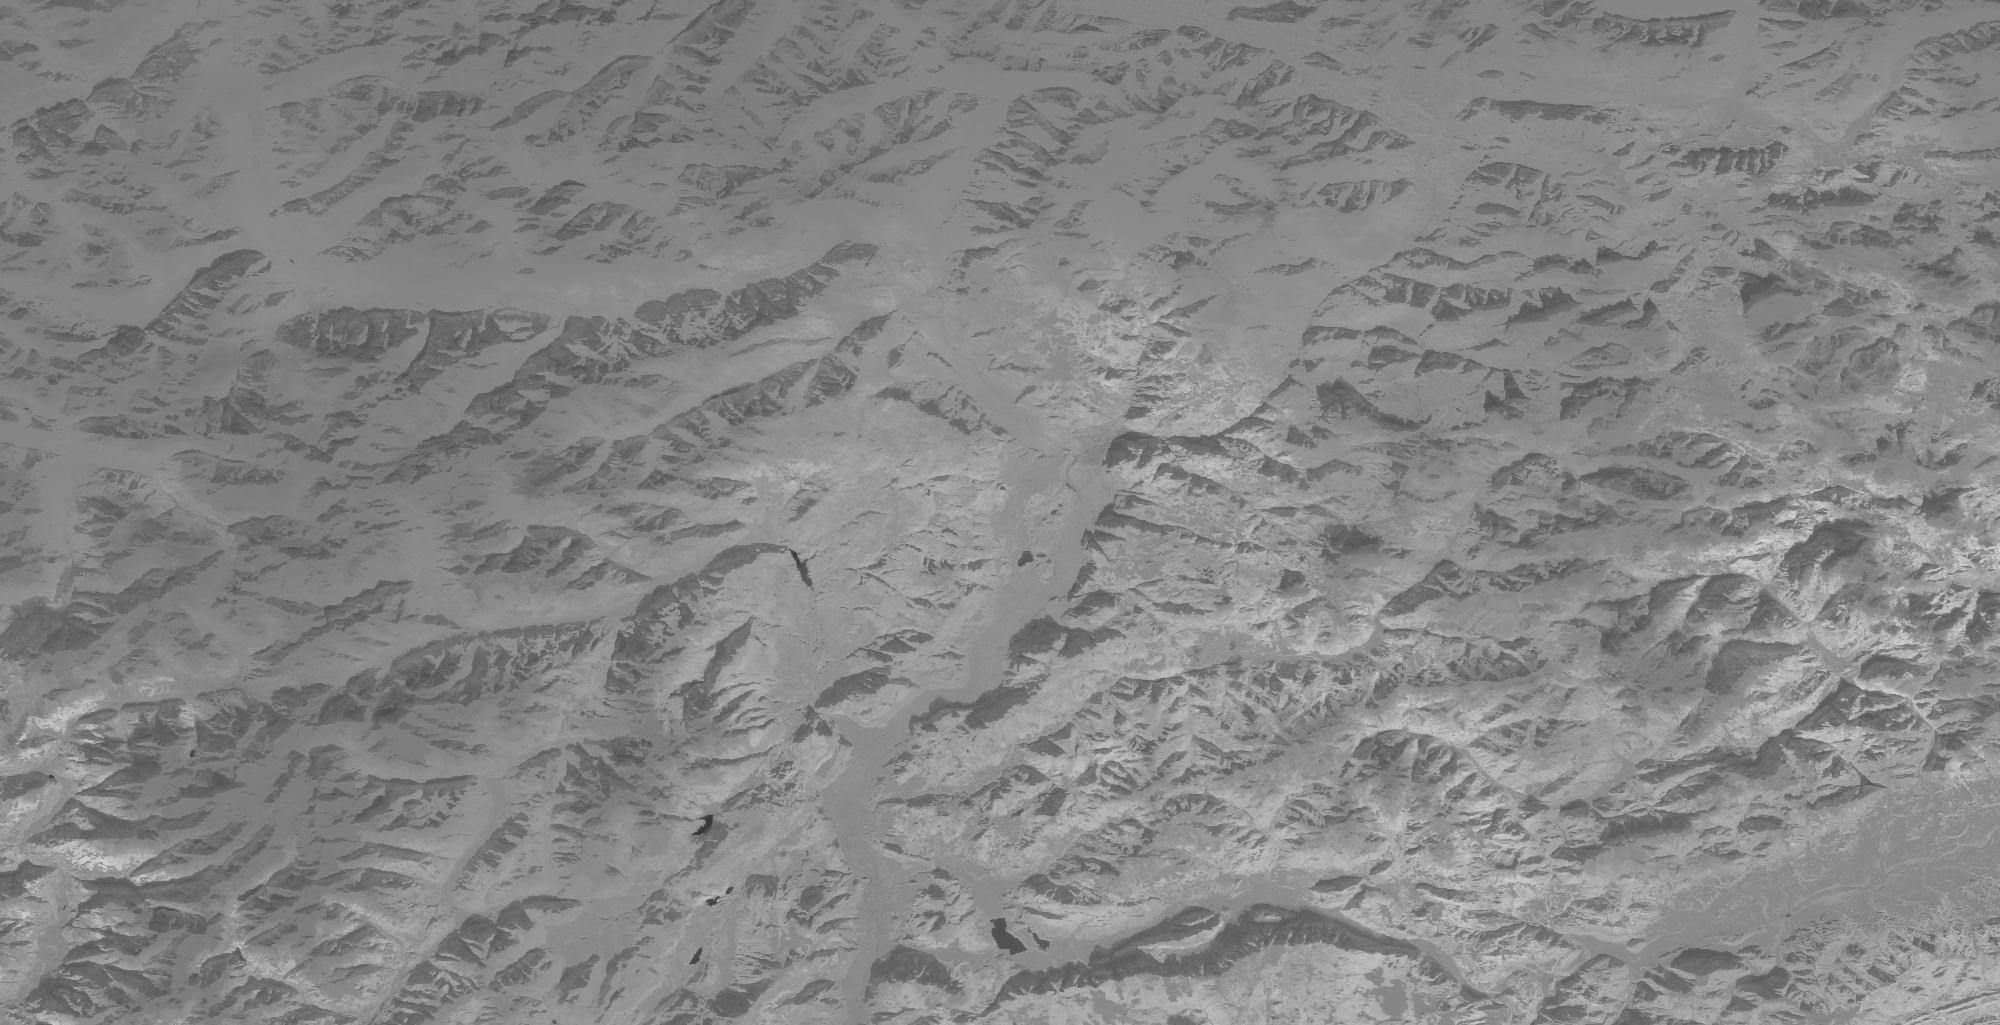
\includegraphics[width=\textwidth]{openeo_example_output}
	\caption{Resulting image of the first step of Use Case 1.}
	\label{fig:impl_usecase1_min} % \label has to be placed AFTER \caption (or \subcaption) to produce correct cross-references.
\end{figure}

	\item \textbf{Researcher A retrieves the used input data of job A.} \\
	If Researcher A wants to receive the input data identifier, the job description endpoint has to be called. The following code snippet shows the call using the python client.

\begin{code}
	\begin{minted}{python}
pidA_url = jobA.get_data_pid_url()
print(pidA_url)
# Output: EODC_DRIVER_URL/data
#	/qu-d1701f4e-e7c5-4a83-92e0-9facbd401a06
pidA = jobA.get_data_pid()

# retrieve information about the pidA 
# e.g. executed query and description about the dataset.
desc = con.describe_collection(pidA)

query = desc["query"]
# re-execute query and get the resulting 
# file list from the backend
file_list = con.get_filelist(pidA)
	\end{minted}
	\caption{Researcher A retrieves the used input data PID.}
	\label{lst:impl_usecase1_2}
\end{code}
	
	\begin{figure}[h]
		\centering
		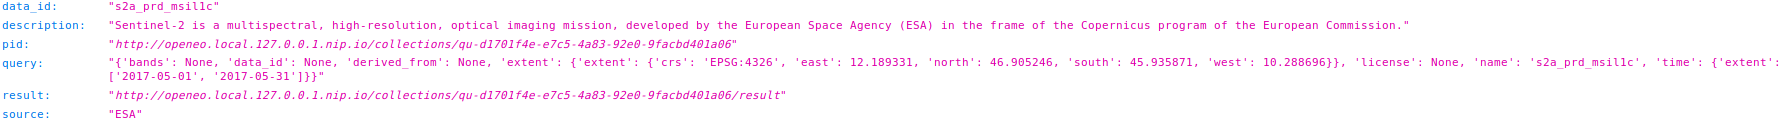
\includegraphics[width=\textwidth]{usecase1_2}
		\caption{Screenshot of the job A landing page.}
		\label{fig:usecase1-pid} % \label has to be placed AFTER \caption (or \subcaption) to produce correct cross-references.
	\end{figure}
	
	The job\_details variable is an unfiltered python dictionary object that contains the response of the EODC backend. It has a data element at the key of "input\_data" that consists of the input data PID as a resolvable web address. Figure \ref{fig:usecase1-pid} shows the response data of the data PID information. After calling the page, the user is provided by the executed filter parameter, the dataset identifier, a description of the dataset. Besides, the link to get the re-execution results of the query and the resolvable data PID is added to the page (see Figure \ref{fig:usecase1-pid}). \\
	The last three calls of the code block above are used to gather the information about the input data directly in the python client code.  
	
	\item \textbf{Researcher A cites the input data in a publication.} \\
	This step is independent from the implementation and therefore not explained in detail. For the further steps it is assumed that Researcher A used the resolvable PID from step 2 (\textit{"EODC\_DRIVER\_URL/data/qu-d1701f4e-e7c5-4a83-92e0-9facbd401a06"}) for the citation.   
	
	\item \textbf{Researcher B uses the same input data of job A for job B.} \\
	To use the same input data as Researcher A, Researcher B uses the data PID from the publication and puts it into the input data element of the process chain of job B. In the block below, an example of the code needed to use the same input with a different process chain (max\_time instead of min\_time process) is printed.  

\begin{code}
	\begin{minted}{python}
import openeo

# Take input data of job A by using the input data PID A
# pidA = qu-d1701f4e-e7c5-4a83-92e0-9facbd401a06
pgB = processes.get_data_by_pid(
data_pid="qu-d1701f4e-e7c5-4a83-92e0-9facbd401a06")
# Alternative: data_pid="EODC_DRIVER_URL/data/pidA" 

# Choose processes
pgB = processes.ndvi(pgB, nir="B08", red="B04")
pgB = processes.max_time(pgB)

# Create job B out of the process graph B (pgB)

jobB = con.create_job(pgB.graph)
jobB.start_job()
	\end{minted}
	\caption{Researcher B uses PID A for different job.}
	\label{lst:impl_usecase1_3}
\end{code}
	
\end{enumerate}

\begin{figure}[h]
	\centering
	
\includegraphics[width=\textwidth]{usecase1_max}
	\caption{Resulting image of the last step of Use Case 1.}
	\label{fig:impl_usecase1_max} % \label has to be placed AFTER \caption (or \subcaption) to produce correct cross-references.
\end{figure}

\subsection{Use Case 2 – Capturing job dependent environments}\label{Implementation:Use Case2}
This scenario focuses on the execution environment. It handles the need for researchers to describe the execution process. Section \ref{UseCase2} describes the second use case in more detail. The implementation at the EODC backend gives the users the option to gain additional data about the execution. In the following, the steps of the scenario are run with the implemented instance of the EODC backend. 

\begin{enumerate}
	\item \textbf{Researcher runs an experiment (job A) at a backend.}\\
	The researcher A runs a job at the EODC backend with the following python client code. It is the default workflow of executing a job using the python client. 

\begin{code}
	\begin{minted}{python}
import openeo
EODC_DRIVER_URL = "http://openeo.local.127.0.0.1.nip.io"

con = openeo.connect(EODC_DRIVER_URL)

# Choose dataset
processes = con.get_processes()
pgA = processes.get_collection(name="s2a_prd_msil1c")
pgA = processes.filter_daterange(pgA, extent=["2017-05-01", 
"2017-05-31"])
pgA = processes.filter_bbox(pgA, west=10.288696, 
south=45.935871, east=12.189331, 
north=46.905246, crs="EPSG:4326")

# Choose processes
pgA = processes.ndvi(pgA, nir="B08", red="B04")
pgA = processes.min_time(pgA)

# Create job A out of the process graph A (pgA)
jobA = con.create_job(pgA.graph)
jobA.start_job()
	\end{minted}
	\caption{Researcher A runs job A with the python client.}
	\label{lst:impl_usecase2_1}
\end{code}
	\item \textbf{Researcher wants to describe the experiment environment.}\\
	The researcher wants to publish the result of the experiment and therefore, needs to describe the environment in detail. The following code-lines provide the user with detailed information about the job execution:

\begin{code}
	\begin{minted}{python}
# Get context model of job A
context_model = jobA.describe_job["context_model"]

# Retrieve the information that Researcher A needs.

interpreter = context_model["interpreter"]
code_env = context_model["code_env"]
input_data = jobA.get_data_pid_url()
backend_version = jobA.get_backend_version()
logging.info("Interpreter: {}".format(interpreter))
logging.info("Code Environment: {}".format(code_env))
logging.info("Input Data PID URL: {}".format(input_data))
logging.info("Back End Version (commit): {}"
             .format(backend_version["commit"]))
	\end{minted}
	\caption{Describe jobA execution environment.}
	\label{lst:impl_usecase2_2}
\end{code}
	After the execution of the lines above, the researcher can get the used programming language, including the version and installed packages. Besides, the backend version describes the used processing code. For more transparency, the researcher can link to the used GitHub repository and the commit to identifying the code. Listing \ref{lst:use_case2_logfile} shows the output of the logging calls.  
	
\end{enumerate}

\begin{code}
	\begin{minted}[fontsize=\footnotesize]{text}
INFO:root:Interpreter: Python 3.7.1
INFO:root:Code Environment: ['alembic==0.9.9', 'amqp==1.4.9',
         ..., 'GitPython==2.1.11', 'numpy==1.16.2', 'GDAL==2.4.0']
INFO:root:Input Data PID URL:
http://openeo.local.127.0.0.1.nip.io/collections
              /qu-8cdac780-7f47-4fac-9c4b-7a9ffff17d1d
INFO:root:Back End Version (commit): 
              16c3b32b5cb2d92d1c32d8c1f929065ee6bf2831
	\end{minted}
	\caption{Logging output of the second Use Case.}
	\label{lst:use_case2_logfile}
\end{code}
%\begin{figure}[h]
%	\centering
%	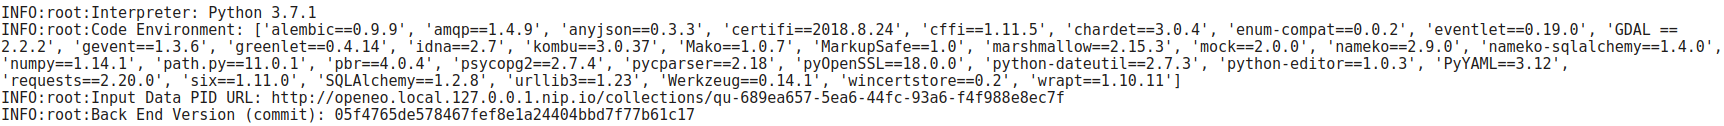
\includegraphics[width=\textwidth]{usecase2_2}
%	\caption{Screenshot of logging output of the second Use Case.}
%	\label{fig:usecase2_2} % \label has to be placed AFTER \caption (or \subcaption) to produce correct cross-references.
%\end{figure}

\subsection{Use Case 3 – Getting differences of job executions}\label{Implementation:Use Case3}
The last use case is focused on the users of openEO. It describes the need for transparency of job executions for the users. If results differ with the same job later in time, the user can access data to find reasons why it happened. Other users might compare different job execution environments. Section \ref{UseCase3} describes the third use case in more detail.  
\begin{enumerate}
	\item \textbf{Researcher runs an experiment (job A) at a backend.}\\
	The researcher A runs a job at the EODC backend with the following python client code. 

\begin{code}
	\begin{minted}{python}
import openeo
EODC_DRIVER_URL = "http://openeo.local.127.0.0.1.nip.io"

con = openeo.connect(EODC_DRIVER_URL)

# Choose dataset
processes = con.get_processes()
pgA = processes.get_collection(name="s2a_prd_msil1c")
pgA = processes.filter_daterange(pgA, extent=["2017-05-01", 
"2017-05-31"])
pgA = processes.filter_bbox(pgA, west=10.288696, 
south=45.935871, east=12.189331, 
north=46.905246, crs="EPSG:4326")

# Choose processes
pgA = processes.ndvi(pgA, nir="B08", red="B04")
pgA = processes.min_time(pgA)

# Create job A out of the process graph A (pgA)

jobA = con.create_job(pgA.graph)
jobA.start_job()
	\end{minted}
	\caption{Researcher A runs job A with the python client.}
	\label{lst:impl_usecase3_1}
\end{code}
	\item \textbf{Researcher re-runs the same experiment (job B).}\\
	Since re-execution of the same job id is handled internally with the re-execution of the same job configuration with a new job id, then the following code is used to create the same job again (job B). It uses the same process graph, and the definition of pgA is the same as in Listing \ref{lst:impl_usecase3_1}:
\begin{code}
	\begin{minted}{python}
jobA = con.create_job(pgA.graph)
jobA.start_job()
	\end{minted}
	\caption{Researcher re-reruns job A resulting in job B.}
	\label{lst:impl_usecase3_2}
\end{code}
	
	\item \textbf{Researcher runs a different experiment (job C).}\\
	The third job (job C) is created with a different process configuration and input data query.

\begin{code}
	%		\inputminted{octave}{BitXorMatrix.m}
	\begin{minted}{python}
# Choose dataset
processes = con.get_processes()
pgC = processes.get_collection(name="s2a_prd_msil1c")
pgC = processes.filter_daterange(pgC, extent=["2017-05-01", 
                                              "2017-05-31"])
pgC = processes.filter_bbox(pgC, west=10.288696, south=45.935871, 
                                 east=12.189331, north=46.905246, 
                                 crs="EPSG:4326")
	
# Choose processes
pgC = processes.ndvi(pgC, nir="B08", red="B04")
pgC = processes.max_time(pgC) # differs from job A
	
# Create job C out of the process graph C (pgC)
	
jobC = con.create_job(pgC.graph)
jobC.start_job()
	\end{minted}
	\caption{Researcher runs experiment different from job A.}
	\label{lst:impl_usecase3_3}
	
\end{code}

	\item \textbf{Researcher wants to compare the jobs by their environment and outcome.}\\
	Now the researcher wants to compare job B and job C with the first job A. Therefore the following code has to be executed:
	
	\begin{code}
%		\inputminted{octave}{BitXorMatrix.m}
		\begin{minted}{python}
diffAB = jobA.diff(jobB)
diffAC = jobA.diff(jobC)
logging.info(diffAB)
logging.info(diffAC)
		\end{minted}
		\caption{Researcher compares the different jobs.}
		\label{lst:impl_usecase3_4}
		
	\end{code}
	 
	With the lines above, the researcher gets two dictionaries of the comparisons between job A with job B (diffAB) and job A with job C (diffAC). The content of the dictionary is a comparison of every key of the jobs context model with each other. Listing \ref{lst:use_case3_logfile} shows the logging output of Listing \ref{lst:impl_usecase3_4}.
\end{enumerate}

%\begin{figure}[h]
%	\centering
%	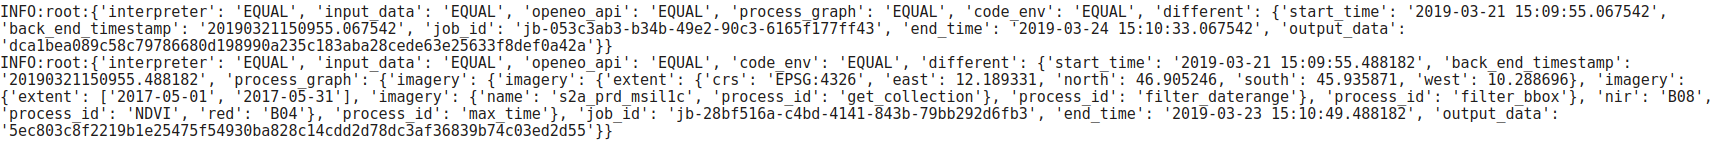
\includegraphics[width=\textwidth]{usecase3_4}
%	\caption{Logging output of the job comparisons diffAB and diffAC.}
%	\label{fig:eva_diff} % \label has to be placed AFTER \caption (or \subcaption) to produce correct cross-references.
%\end{figure}

\begin{code}
	\begin{minted}[fontsize=\footnotesize]{text}
INFO:root:{'input_data': 'EQUAL', 'output_data': 'EQUAL', 
 'process_graph': 'EQUAL', 'openeo_api': 'EQUAL', 
 'interpreter': 'EQUAL', 'code_env': 'EQUAL',
 'different': 
 {'back_end_timestamp': '20190417194702.496810', 
 'job_id': 'jb-b92c688c-7fdc-4126-bcdf-85bc07030237', 
 'start_time': '2019-04-17 19:47:02.496810', 
 'end_time': '2019-04-17 19:47:03.258261'}} 
INFO:root:{'input_data': 'EQUAL', 'output_data': 'EQUAL', 
 'openeo_api': 'EQUAL', 'interpreter': 'EQUAL', 'code_env': 'EQUAL',
 'different': {'process_graph': {'imagery': {'imagery': {'extent': 
 {'crs': 'EPSG:4326', 'east': 12.189331, 'north': 46.905246, 
 'south': 45.935871, 'west': 10.288696}, 'imagery': 
 {'extent': ['2017-05-01', '2017-05-31'], 
 'imagery': {'name': 's2a_prd_msil1c', 'process_id': 'get_collection'}, 
 'process_id': 'filter_daterange'}, 'process_id': 'filter_bbox'}, 
 'nir': 'B08', 'process_id': 'NDVI', 'red': 'B04'}, 'process_id': 
 'max_time'}, 'start_time': '2019-04-17 19:47:09.089075', 
 'end_time': '2019-04-17 19:47:11.786845', 
 'back_end_timestamp': '20190417194709.089075', 
 'job_id': 'jb-ecdd5768-3c22-4c73-85b8-ac6f4bdc138f'}}
	\end{minted}
	\caption{Logging output of the job comparisons diffAB and diffAC.}
	\label{lst:use_case3_logfile}
\end{code}

\section{Summary}
This chapter presented an implementation of the design of Chapter \ref{Design} at the EODC backend. It consists of an implementation of the RDA recommendations for the backend. The additional modules needed to achieve this are presented in Section \ref{Implementation:Data Identification} and are using the CSW\footnote{http://cite.opengeospatial.org/pub/cite/files/edu/cat/text/main.html} query system. The implementation of the backend provenance uses the advantages of GitHub on versioning the used software and persisting the software versions of the past. The job dependent environment is captured by retrieving the python environment using pip and capturing the version of the software at the execution time. The logging system of the EODC backend is used to communicate the data needed by the context model without changing the processing code. The data of the query and the context model are persisted in additions to the existing PostgreSQL database. Besides, the endpoints needed to access the provenance information are inserted into the openEO API. In the last section of the chapter, the implementation of the defined Use Cases of Section \ref{Use Cases} are presented. The next chapter evaluates the implementation by the impact on the EODC backend and by testing the implementation against exceptional cases.   

\chapter{Evaluation}\label{Evaluation}
\todo{Always "the backend" not "the EODC backend", just in the first mentioning of the section}

\todo{Gesamte Thesis: Present simple \& Past simple and not "could / would" So: we have implemented --> we implemented}
\todo{Gesamte Thesis: Restructure passive sentences}
\todo{Gesamte Thesis:Konsistente Verwendung von Begriffen --> Glossary ?? --> workflow (Beschreibung des Experiments aus sicht des wissenschaftlers), job (Definition des im backend durchgeführten parts), workflow, process graph (technische Beschreibung bzw. Definition des jobs)}
\todo{Gesamte Thesis: Wortwiederholungen sind gut !!}
\todo{Gesamte Thesis: Unnötige Wörter / Sätze weg z.b. briefly, some, also, ...}
\todo{Gesamte Thesis: Kurze einfache Sätze}
\todo{Gesamte Thesis: Eher Reproducibility schreiben in den Allgemeinen Kapiteln, aber in den RQ repeatability schreiben}
\todo{Gesamte Thesis: Software --> Environment / Code ? --> just check correct usage}
This chapter evaluates the concept of the prototype implementation described in Chapter \ref{Implementation}. The solution is evaluated by test cases that simulate updates on data as well as on the backend environment. The performance and storage impact of the solution is evaluated by applying 18 test cases derived from 9 publications that used EODC data in the past. The chapter is structured as follows: \\
First, the set up of the evaluation environment is described in Section \ref{Evaluation:Setup}. Section \ref{Evaluation:special_dataid} evaluates how the solution behaves on data updates at the backend. The following Section \ref{Evaluation:special_jobcap}  evaluates if the recreation of an older back end version is possible using the solution. Section \ref{Evaluation:impact} provides measurements on the performance and storage impact of the solution system. 

\section{Evaluation Setup}\label{Evaluation:Setup}

EODC uses an OpenShift\footnote{https://www.openshift.com/} service to provide the backends functionality. For this evaluation, OpenShift is installed locally to run the solution backend. Nevertheless, the data querying of EODC is publicly available and is used. The \textit{Query Handler} component of the solution is operating with the actual data that EODC provides for openEO users. \\
The processing service of EODC cannot be executed locally because the data files are only inside of the EODC infrastructure available. Therefore, the processing mechanism is mocked up. The mockup creates an array with mockup values in the size of the query results and applies the defined processes of the process graph on it. To be able to run test cases independently, a "reset" endpoint is added to the backend. After calling it, all stored job and query records are deleted from the database. Figure \ref{fig:evaluation_setup} gives an overview of the evaluation setup. \\
Table \ref{Tab:eva_hardware} specifies the local machine used for the evaluation. To get a minimum performance bias, not necessary background programs are disabled for the evaluation execution.\\  
The evaluation is done from a user point of view, hence the openEO python client with the additions of Section \ref{Implementation:User Interface} is used for the evaluation. The python client, the solution backend, and the code for the evaluation is available and further described on GitHub\footnote{https://github.com/bgoesswein/dataid\_openeo}. 

\begin{figure}[h]
	\centering
	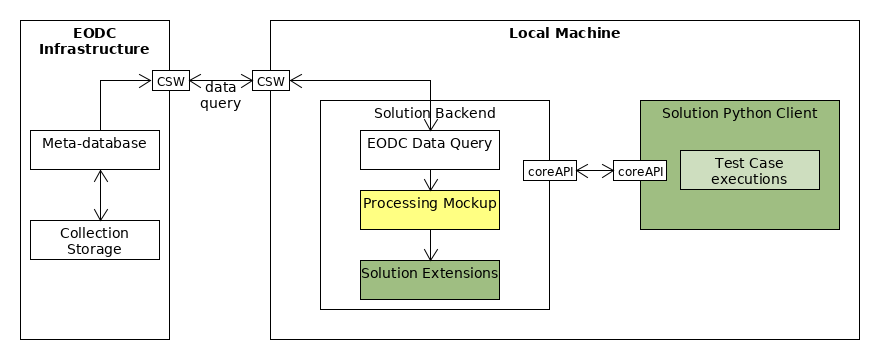
\includegraphics[scale=0.46]{evaluation_setup}
	\caption{Overview of the evaluation setup.}
	\label{fig:evaluation_setup} % \label has to be placed AFTER \caption (or \subcaption) to produce correct cross-references.
\end{figure}

\begin{table}[]
	\caption{Evaluation system specifications.}
	\centering
	\begin{tabular}{l|l}
		\multicolumn{2}{c}{\textbf{Hardware}} \\ \hline
		\textbf{\acrshort{cpu}} & Intel(R) Core(TM) i7-3770T CPU @ 2.50GHz \\ 
		\textbf{\acrshort{gpu}} & Radeon HD 7750/8740 / R7 250E  \\ 
		\textbf{\acrshort{ram}} & 16 GB  \\ 
		\multicolumn{2}{c}{\textbf{Software}} \\ \hline
		\textbf{\acrshort{os}} & Kubuntu 18.04.1 LTS \\ 
		\textbf{OpenShift} & 3.9.0  \\ 
		\textbf{Python} & 3.7.1  \\ 
	\end{tabular}
	\label{Tab:eva_hardware}
\end{table}

%\section{Special Test Cases}\label{Evaluation:special}
%This section evaluates special test cases to get an overview on how the solution behaves, if special circumstances on the backend occur. The GitHub repository of the solution has unit tests in the "test" folder of the python client testing the basic functionality. The test cases in this section are created to look into the error proneness of the solution. The code as well as the results of the evaluation in this section are available on GitHub\footnote{https://github.com/bgoesswein/dataid\_openeo/tree/master/openeo-python-client/examples/}.

\section{Data Identification}\label{Evaluation:special_dataid}
This section evaluates the data identification mechanism that is a proposed extension to a backend. We first show how the solution fulfills the \acrshort{rda} recommendations and later how the solution behaves if data updates or deletions occur at the back end.\\  
The policy of the EODC backend regarding updates on data sets is dependent on the type of data:

\begin{enumerate}
	\item \textbf{Sentinel Data} \\
	The Sentinel data, which is used by EODC for the openEO project, has never been updated before. The data comes directly from ESA, and updated datasets from ESA were not applied to the EODC data yet. However, the occurrence of updates is, in general, not forbidden in future of the EODC backend. If a dataset were updated, it would follow the updated policy of ESA, therefore having a new file name for the updated file. Hence, updates on the data can be simulated by renaming the input files and the creation timestamp. Other than updating the existing datasets, there are regular updates on the extent of the Sentinel data sets.   
	\item \textbf{Processed Data} \\
	Data that is processed by partners of EODC is maintained and therefore also updated by the partners. Old versions of this data are deleted or archived by EODC, depending on the decision of the partner. This type of data is not available using openEO since it is the property of the partners and not EODC. Besides, to be able to use the same processes on different openEO backends, the standard data layer needs to be the same. That is why only unprocessed data is used by all backends contributing to openEO. Since the data sets are not available for openEO, the data identification of them is not in the scope of the thesis. By now, EODC plans to use the openEO framework for their whole infrastructure, which brings the partners to use openEO for their processing. Therefore they can use the data identification implementation for their tasks.
\end{enumerate}

\subsection{RDA Recommendations}\label{Evaluation:dataidentification}
The Design (Section \ref{Design:Data Identification}) defines that the backend needs to implement the \acrshort{rda} data identification recommendations. Therefore the following enumeration shows how the recommendations are achieved in this implementation. 

\begin{itemize}
	\item \textbf{R1: Data Versioning} \\
	The EODC backend has versioning of data already implemented, by following the naming policies of ESA. The path to the file is the version identifier since modified files must have a different file name.
	\item \textbf{R2: Timestamping} \\
	The creation timestamp of the files are stored by the file system of EODC since the files have to change the name after an update, the creation timestamp of the updated file is the update timestamp of the original file. 
	\item \textbf{R3: Query Store Facilities} \\
	A new table implements the query store in the EODC database (PostgreSQL) used for openEO. The query Table stores the following data about each query:
	\begin{itemize}
		\item The original executed \acrshort{csw} query in XML format
		\item The unique query is generated out of the JSON object created by the EODC backend after parsing the filter arguments of the process graph. To assure uniqueness the JSON is sorted alphabetically.
		\item Hash of the unique query after removing all characters with no semantic meaning from it.
		\item Hash of the alphabetically sorted resulting file list after removing all characters with no semantic meaning from it. 
		\item Timestamp of the original query execution.
		\item Dataset identifier is set to the used collection identifier of the query.
		\item Generated persistent identifier of the query using the uuid library of python.
		\item JSON object with the number of result files.
	\end{itemize}
	\item \textbf{R4: Query Uniqueness} \\
	The alphabetically sorted filter JSON object provided by the EODC backend (See Figure \ref{fig:processgraph_example}).
	\item \textbf{R5: Stable Sorting} \\
	The original \acrshort{csw} query assures stable sorting. It sorts the resulting file list in ascending order (alphabetically).
	\item \textbf{R6: Result Set Verification} \\
	The resulting file list is a list sorted alphabetically in ascending order. It transfers to a string object that gets cleaned up by characters that are not relevant, before being hashed by the SHA-256 hash function. 
	\item \textbf{R7: Query Timestamping} \\
	The implementation stores the timestamp of the original query execution. 
	\item \textbf{R8: Query PID}\\
	The query PID is getting created (using Python UUID\footnote{https://docs.python.org/3/library/uuid.html}) if the same unique query and the resulting hash combination is not in the database yet.
	\item \textbf{R9: Store the Query} \\
	The Query Store is implemented as an additional table of an already existent relational database of EODC for openEO (PostgreSQL). 
	\item \textbf{R10: Automated Citation Texts} \\
	The citation text for the data-set is already available at EODC, the generated data PID is added to it. 
	\item \textbf{R11 \& R12: Landing Page \& Machine Actionability} \\
	The EODC backend defines the landing page as an openEO endpoint. It is publicly accessible and in a JSON format, which makes it machine actionable. The landing page consists of an additional link to re-execute the query and lists the result files. Since it is part of the openEO API, it can also be accessed from the openEO clients and be used in future jobs as input data.
	\item \textbf{R13 \& R14: Technology Migration \& Migration Verification} \\
	These recommendations are not implemented in this thesis since there are no migrations planned at EODC.
\end{itemize}

The test cases of the following sections focus on the Sentinel Data of EODC, and how the solution handles data updates. The running job (referenced as jobA) defined in Section \ref{example} is used for this evaluation. At the beginning of each test case, the first step is to run a job on the empty database to create the first query Table entry. 

\subsection{Test Case Preparation}
This section describes the first step of each test case in the following sections. The purpose is to add a first job execution with an input data PID, which is needed for each test scenario. Before this step is executed, the database of the backend is cleaned up.\\ The original data of EODC cannot be changed for this evaluation since the evaluation backend is using the actual data endpoint (https://csw.eodc.eu). To simulate changes on the data, the query result received by the backend driver gets modified. Figure \ref{fig:eva_data_simulation} gives an overview of where the data update simulator is located in the data identification implementation overview of Figure \ref{fig:impldataid}. The test cases below describe what data is modified. \\

\begin{figure}[h]
	\centering
	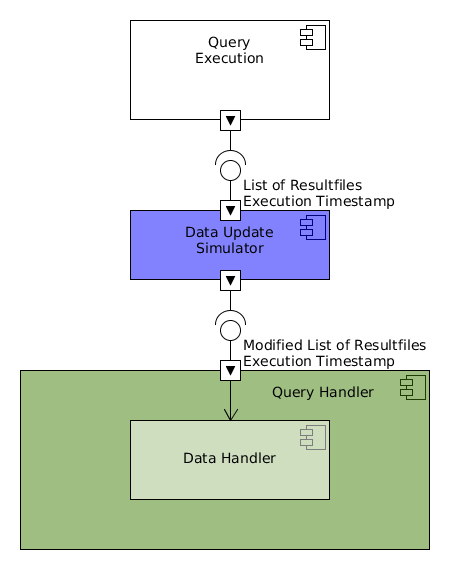
\includegraphics[scale=0.4]{evaluation_data_simulation}
	\caption{Overview of the data update simulation. It shows the extension on the data identification implementation of Figure \ref{fig:impldataid}.}
	\label{fig:eva_data_simulation} % \label has to be placed AFTER \caption (or \subcaption) to produce correct cross-references.
\end{figure}

\begin{enumerate}
	\item \textbf{Run jobA, which creates query pidA. Get result files of pidA} \\
	Listing \ref{lst:eva_datachange_1} shows the code to run jobA using the python client. The researcher defines the spatial and temporal filter arguments and applies the NDVI and the minimum time process on it, described in Section \ref{example}. The "con.create\_job()" line sends the process graph to the backend and retrieves a job object containing the newly generated job id. After executing jobA (calling start\_job()), a job entity and a query entity are created and persisted in the database. The query entity with a generated data PID is created by the \textit{Query Handler}, since the database has no query entry. Table \ref{Tab:eva_datachanges1} shows the state of the \textit{Query} table after the execution of the following python code.
	\begin{code}
		\begin{minted}[fontsize=\small]{python}
		con = openeo.connect("http://openeo.local.127.0.0.1.nip.io")
# Choose dataset
processes = con.get_processes()
pgA = processes.get_collection(name="s2a_prd_msil1c")
pgA = processes.filter_daterange(pgA, extent=["2017-05-01", "2017-05-31"])
pgA = processes.filter_bbox(pgA, west=10.288696, south=45.935871, 
east=12.189331, north=46.905246, crs="EPSG:4326")
# Choose processes
pgA = processes.ndvi(pgA, nir="B08", red="B04")
pgA = processes.min_time(pgA)
# Create and start job A out of the process graph A (pgA)
jobA = con.create_job(pgA.graph)
jobA.start_job()
# Get data PID of jobA
pidA = jobA.get_data_pid()
# Re-execute the query to print the used files.
file_listA = con.get_filelist(pidA)
# Get state of the resultfiles, so if they changed since 
# the original execution 
file_listA["input_files"]["state"] # Returns "EQUAL"
		\end{minted}
		\caption{Researcher runs jobA and retrieves the result files status.}
		\label{lst:eva_datachange_1}
	\end{code}
	Figure \ref{fig:eva_data_changes_1_query} shows the original query that got executed at the backend. It is an XML schema consisting of the filter values defined in the process graph (pgA). The figure of the query highlights the timestamp of the first query execution. The content of the database tables as well as query re-execution results after each execution step are available in the result folder\footnote{https://github.com/bgoesswein/dataid\_openeo/tree/master/openeo-python-client/examples/results} of the GitHub repository. 
	
	\begin{figure}[h]
		\centering
		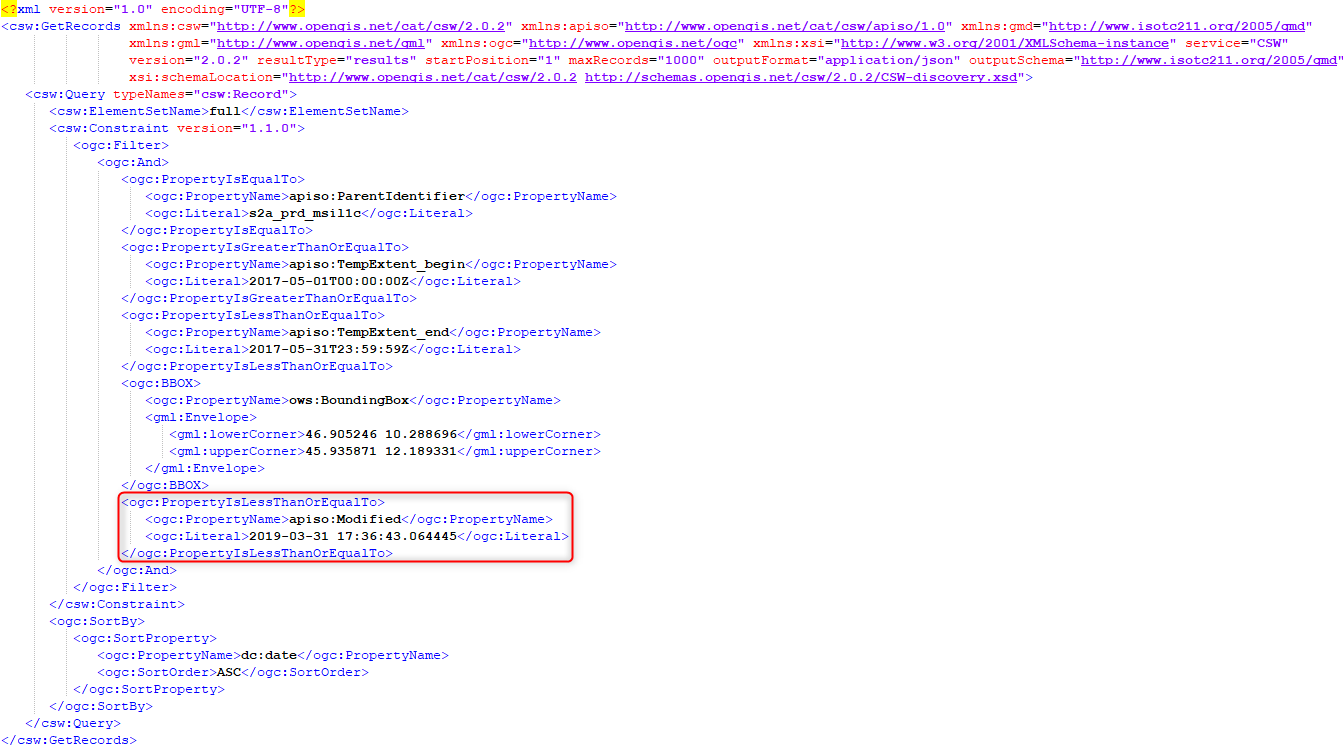
\includegraphics[width=\textwidth]{eva_data_changes_1_query}
		\caption{Original query of jobA at the first evaluation step.}
		\label{fig:eva_data_changes_1_query} % \label has to be placed AFTER \caption (or \subcaption) to produce correct cross-references.
	\end{figure}
	
	Listing \ref{lst:eva_datachange_nq1} shows the normalized query created by the \textit{Query Handler}. It contains all possible filter arguments and their values in a JSON object alphabetically sorted.
	
	\begin{code}
		\begin{minted}[fontsize=\footnotesize]{text}
{'bands': None, 
'data_id': None, 
'derived_from': None, 
'extent': {'extent': {'crs': 'EPSG:4326', 'east': 12.189331, 
'north': 46.905246, 'south': 45.935871, 'west': 10.288696}}, 
'license': None, 
'name': 's2a_prd_msil1c', 
'time': {'extent': ['2017-05-01', '2017-05-31']}}
		\end{minted}
		\caption{Normalized query of the first query entry.}
		\label{lst:eva_datachange_nq1}
	\end{code}
	
	Listing \ref{lst:eva_datachange_rf1} shows the first four file paths and timestamps of the resulting file list, after executing the query in Figure \ref{fig:eva_data_changes_1_query}. The resulting file list (file\_listA["input\_files"]) consists of 51 files and the re-execution of the query results in the same 51 files. The path of each file contains data about the data record. The term "s2a\_prd\_msil1c" defines the dataset identifier of Sentinel 2 at EODC. The following folders define the date of the data record. The filename follows the ESA naming convention\footnote{https://sentinel.esa.int/web/sentinel/user-guides/sentinel-2-msi/naming-convention}. The Nxxyy value defines the baseline number, Rxxx defines the orbit number of the satellite and Txxxxx defines the tile number. The first date is the sensing time and the second at the end of the file name is the product disclaimer, therefore identifies products that came from the data of the same sensing time. The timestamp entry shows when the data was first available at EODC.
	
	\begin{code}
		\begin{minted}[fontsize=\footnotesize]{text}
{'timestamp': '2017-05-08 00:00:00', 
'path': '/eodc/products/copernicus.eu/s2a_prd_msil1c/2017/05/04/
S2A_MSIL1C_20170504T101031_N0205_R022_T32TPR_20170504T101349.zip'}, 
{'timestamp': '2017-05-08 00:00:00',
'path':'/eodc/products/copernicus.eu/s2a_prd_msil1c/2017/05/04/
S2A_MSIL1C_20170504T101031_N0205_R022_T32TQS_20170504T101349.zip', 
{'timestamp': '2017-05-08 00:00:00', 
'path': '/eodc/products/copernicus.eu/s2a_prd_msil1c/2017/05/04/
S2A_MSIL1C_20170504T101031_N0205_R022_T32TQR_20170504T101349.zip'}, 
{'timestamp': '2017-05-08 00:00:00',
'path':'/eodc/products/copernicus.eu/s2a_prd_msil1c/2017/05/04/
S2A_MSIL1C_20170504T101031_N0205_R022_T32TPT_20170504T101349.zip'},
...
		\end{minted}
		\caption{First four resulting files of the file list.}
		\label{lst:eva_datachange_rf1}
	\end{code}
	
	Table \ref{Tab:eva_datachanges1} shows the content of the \textit{Query} table after the execution of this step. There is one entry with a new generated data PID, by the \textit{Query Handler}, since there was no query entry in the database that matches the normalized hash and the resulting hash.
	
	%\begin{table}[]
	%	\caption{\textit{Query} table after the execution of Listing \ref{lst:eva_datachange_1}}
	%	\begin{tabular}{|l|l|l|l|l|l|l|l|l|}
	%		\hline	\textbf{query\_pid} & \textbf{dataset\_pid} & \textbf{original} & \textbf{normalized} & \textbf{norm\_hash} & \textbf{result\_hash} &
	%		\textbf{updated\_at} & \textbf{meta\_data} &   
	%		\textbf{created\_at} \\ \hline
	%		qu-a3bbe4a0-a875-4687-bb78-9457f33134a9 & s2a\_prd\_msil1c & see Figure \ref{fig:eva_data_changes_1_query} & see Listing \ref{lst:eva_datachange_nq1} & 0917c7a21cec960b8a6617b22ad26578c2c67f0b0501ba1a359b078c6c51d77d & abf43f519007050cbaeb59a067a2226d64b041c6d6ec323b2401109176e66455 & 2019-03-31 17:36:44.613893 & {'result\_files': 51} & 2019-03-31 17:36:43.064445 \\ \hline
	%	\end{tabular}
	%	\label{Tab:eva_datachanges1}
	%\end{table}
	
	\begin{table}[]
		\caption{\textit{Query} table after the execution of Listing \ref{lst:eva_datachange_1}}
		\centering
		\begin{tabular}{|r|l|}
			\hline \multicolumn{2}{|c|}{\textbf{Query pidA}} \\
			\hline \multicolumn{1}{|c|}{\textbf{Column}}  &  \multicolumn{1}{c|}{\textbf{Value}} \\ \hline
			query\_pid & qu-a3bbe4a0-a875-4687-bb78-9457f33134a9  \\ 
			dataset\_pid & s2a\_prd\_msil1c  \\ 
			original & see Figure \ref{fig:eva_data_changes_1_query}   \\
			normalized & see Listing \ref{lst:eva_datachange_nq1}  \\
			norm\_hash & 0917c7a21cec960b8a6617b22ad26578c2c67f0b0501ba1a359b078c6c51d77d  \\
			result\_hash & abf43f519007050cbaeb59a067a2226d64b041c6d6ec323b2401109176e66455   \\
			updated\_at & 2019-03-31 17:36:44.613893   \\
			meta\_data & {'result\_files': 51}  \\
			created\_at & 2019-03-31 17:36:43.064445   \\ \hline
		\end{tabular}
		\label{Tab:eva_datachanges1}
	\end{table}
\end{enumerate}

\subsection{Test Case 1: Is it possible to re-execute a query after a file is updated?}	\label{Tab:eva_datachanges_tc1}
%{ \large \textbf{} } \\

\begin{enumerate}
	\setcounter{enumi}{+1}
	\item \textbf{Update one of the resulting files of the pidA query} \\
	The "update\_file()" method is added to the python client and EODC backend to let the backend activate the "Data Update Simulator" shown in Figure \ref{fig:eva_data_simulation}. If it is activated, it simulates the update of the first file in the query result. The update sets the creation timestamp of the file to the execution time of the "update\_file()" method and renames the updated output file with an additional "\_new". The update does not replace the old file but adds a new file to the result.
	\begin{code}
		\begin{minted}[fontsize=\small]{python}
# Update the first file of the pidA query resulting files.
con.update_file()
		\end{minted}
		\caption{Update one of the pidA resulting files, but keep the original file.}
		\label{lst:eva_datachange_2}
	\end{code}
	
	Listing \ref{lst:eva_datachange_fl2} shows the resulting file list with the activated "Data Update Simulator". There is now an additional file with an "\_new" at the end of the path, but with the same data in the file path and name as the first file. Besides, the creation timestamp is set to the time of the execution of Listing \ref{lst:eva_datachange_2}.
	
	\begin{code}
		\begin{minted}[fontsize=\small]{text}
{'timestamp': '2017-05-08 00:00:00', 
'path': '/eodc/products/copernicus.eu/s2a_prd_msil1c/2017/05/04/
S2A_MSIL1C_20170504T101031_N0205_R022_T32TPR_20170504T101349.zip'}, 
{'timestamp': '2019-03-31 17:44:43', 
'path': '/eodc/products/copernicus.eu/s2a_prd_msil1c/2017/05/04/
S2A_MSIL1C_20170504T101031_N0205_R022_T32TPR_20170504T101349_new.zip'}
{'timestamp': '2017-05-08 00:00:00',
'path':'/eodc/products/copernicus.eu/s2a_prd_msil1c/2017/05/04/
S2A_MSIL1C_20170504T101031_N0205_R022_T32TQS_20170504T101349.zip', 
{'timestamp': '2017-05-08 00:00:00', 
'path': '/eodc/products/copernicus.eu/s2a_prd_msil1c/2017/05/04/
S2A_MSIL1C_20170504T101031_N0205_R022_T32TQR_20170504T101349.zip'}, 
{'timestamp': '2017-05-08 00:00:00',
'path':'/eodc/products/copernicus.eu/s2a_prd_msil1c/2017/05/04/
S2A_MSIL1C_20170504T101031_N0205_R022_T32TPT_20170504T101349.zip'},
...
		\end{minted}
		\caption{Modified file list output of the "Data Update Simulator" component.}
		\label{lst:eva_datachange_fl2}
	\end{code}
	
	\item \textbf{Re-execution of pidA query} \\
	In Listing \ref{lst:eva_datachange_3} the query with the identifier pidA gets re-executed, after the activation of the "Data Update Simulator" component in the previous step. The second query re-execution results in the same file list as the first (see Listing \ref{lst:eva_datachange_rf3}), since the old file is still available and the updated file is added after the execution timestamp of the first execution (see timestamp element in the query at Figure \ref{fig:eva_data_changes_1_query}). The query contains the execution timestamp of the original query and filters every file out of the result that has a creation timestamp after that.
	\begin{code}
		\begin{minted}[fontsize=\small]{python}
# Get state of the resultfiles, so if they changed since 
# the original execution. 
file_listA = con.get_filelist(pidA)
file_listA["input_files"]["state"] # Returns "EQUAL"
		\end{minted}
		\caption{Re-execute pidA query after one file got updated.}
		\label{lst:eva_datachange_3}
	\end{code}
	
	\begin{code}
		\begin{minted}[fontsize=\footnotesize]{text}
{'timestamp': '2017-05-08 00:00:00', 
'path': '/eodc/products/copernicus.eu/s2a_prd_msil1c/2017/05/04/
S2A_MSIL1C_20170504T101031_N0205_R022_T32TPR_20170504T101349.zip'}, 
{'timestamp': '2017-05-08 00:00:00',
'path':'/eodc/products/copernicus.eu/s2a_prd_msil1c/2017/05/04/
S2A_MSIL1C_20170504T101031_N0205_R022_T32TQS_20170504T101349.zip', 
{'timestamp': '2017-05-08 00:00:00', 
'path': '/eodc/products/copernicus.eu/s2a_prd_msil1c/2017/05/04/
S2A_MSIL1C_20170504T101031_N0205_R022_T32TQR_20170504T101349.zip'}, 
{'timestamp': '2017-05-08 00:00:00',
'path':'/eodc/products/copernicus.eu/s2a_prd_msil1c/2017/05/04/
S2A_MSIL1C_20170504T101031_N0205_R022_T32TPT_20170504T101349.zip'},
...
		\end{minted}
		\caption{First four resulting files of the file list.}
		\label{lst:eva_datachange_rf3}
	\end{code}
	
	\item \textbf{Run duplicate of jobA named jobB} \\
	Listing \ref{lst:eva_datachange_4} shows the execution of a second job using the same process graph as jobA. In the first line of Listing \ref{lst:eva_datachange_4} the process graph of jobA (defined in Listing \ref{lst:eva_datachange_1}) is used to create a new job instance named jobB. Therefore, jobB uses the same process graph as jobA but gets executed after the update of the file. It leads to a different file list, where the original and the new file is in the query result file list (see Listing \ref{lst:eva_datachange_fl3}).
	\begin{code}
		\begin{minted}[fontsize=\small]{python}
# Reuse the defined process Graph (pgA) from jobA at Step 1 to create jobB
jobB = con.create_job(pgA.graph)
jobB.start_job()
# re-execute query and get the resulting file list from the backend
pidB = jobB.get_data_pid()
file_listB = con.get_filelist(pidB)
# comparing the resultfiles of jobA with the resultfiles of jobB
(file_listA == file_listB) # Returns False
		\end{minted}
		\caption{Step 4: Create jobB, which uses the same process graph as jobA.}
		\label{lst:eva_datachange_4}
	\end{code}
	
	\begin{code}
		\begin{minted}[fontsize=\small]{text}
{'timestamp': '2017-05-08 00:00:00', 
'path': '/eodc/products/copernicus.eu/s2a_prd_msil1c/2017/05/04/
S2A_MSIL1C_20170504T101031_N0205_R022_T32TPR_20170504T101349.zip'}, 
{'timestamp': '2019-03-31 17:44:43', 
'path': '/eodc/products/copernicus.eu/s2a_prd_msil1c/2017/05/04/
S2A_MSIL1C_20170504T101031_N0205_R022_T32TPR_20170504T101349_new.zip'}
{'timestamp': '2017-05-08 00:00:00',
'path':'/eodc/products/copernicus.eu/s2a_prd_msil1c/2017/05/04/
S2A_MSIL1C_20170504T101031_N0205_R022_T32TQS_20170504T101349.zip', 
{'timestamp': '2017-05-08 00:00:00', 
'path': '/eodc/products/copernicus.eu/s2a_prd_msil1c/2017/05/04/
S2A_MSIL1C_20170504T101031_N0205_R022_T32TQR_20170504T101349.zip'}, 
{'timestamp': '2017-05-08 00:00:00',
'path':'/eodc/products/copernicus.eu/s2a_prd_msil1c/2017/05/04/
S2A_MSIL1C_20170504T101031_N0205_R022_T32TPT_20170504T101349.zip'},
...
		\end{minted}
		\caption{Resulting file list of jobB.}
		\label{lst:eva_datachange_fl3}
	\end{code}
	
	Table \ref{Tab:eva_datachanges3} shows the \textit{Query} table of the database after the execution of Listing \ref{lst:eva_datachange_4}. There is now an additional query entry. In the table, the important differences are marked red. There is a different result hash since the number of result files has increased (see Listing \ref{lst:eva_datachange_fl3}). The normalized query is still the same, but since the result of the query changed, a new data PID is generated. 
	
	\begin{table}[]
		\caption{\textit{Query} table after the execution of Listing \ref{lst:eva_datachange_4}. Important elements are highlighted blue if they are the same and red if they are different.}
		\centering
		\begin{tabular}{|r|l|}
			\hline \multicolumn{2}{|c|}{\textbf{Query pidA (full entry in Table \ref{Tab:eva_datachanges1})}} \\
			\hline \multicolumn{1}{|c|}{\textbf{Column}}  &  \multicolumn{1}{c|}{\textbf{Value}} \\ \hline
			query\_pid & {\color{red}qu-a3bbe4a0-a875-4687-bb78-9457f33134a9}  \\ 
			norm\_hash & {\color{blue}0917c7a21cec960b8a6617b22ad26578c2c67f0b0501ba1a359b078c6c51d77d}  \\
			result\_hash & {\color{red}abf43f519007050cbaeb59a067a2226d64b041c6d6ec323b2401109176e66455}   \\
			meta\_data & {'result\_files': 51}  \\
			\hline \multicolumn{2}{|c|}{\textbf{Query pidB}} \\
			\hline \multicolumn{1}{|c|}{\textbf{Column}}  &  \multicolumn{1}{c|}{\textbf{Value}} \\ \hline
			query\_pid & { \color{red} qu-23f5a313-e804-4faa-aa33-60ed1ac69e2d}  \\ 
			dataset\_pid & s2a\_prd\_msil1c  \\ 
			original & see Figure \ref{fig:appendix_pidB} in the appendix \\
			normalized & see Listing \ref{lst:eva_datachange_nq1}  \\
			norm\_hash & {\color{blue}0917c7a21cec960b8a6617b22ad26578c2c67f0b0501ba1a359b078c6c51d77d}  \\
			result\_hash & {\color{red}28088d113de19ce037e9651a64bae3f7957822665f17d8f4e2c7e6b2cf4250b3 }  \\
			updated\_at & 2019-03-31 18:01:49.214956   \\
			meta\_data & {\color{red}'result\_files': 52}  \\
			created\_at & 2019-03-31 18:01:47.695042   \\ \hline
		\end{tabular}
		\label{Tab:eva_datachanges3}
	\end{table}
	
	\item \textbf{Run duplicate of jobA, by using the data PID of jobA named jobC}\\
	The persistent input data identifier of job A (pidA) is used as the input data to create jobC. The execution timestamp is part of the query in pidA, and the original query gets executed for jobC. Since jobC uses the same data PID as jobA, the updated file is filtered out of the resulting files, and there is no new data PID generated. Therefore, the \textit{Query} table is still in the state of Table \ref{Tab:eva_datachanges3}. 
	\begin{code}
		\begin{minted}[fontsize=\small]{python}
# Take input data of job A by using the input data PID A of job A
pgC = processes.get_data_by_pid(data_pid=pidA)
# Choose processes
pgC = processes.ndvi(pgC, nir="B08", red="B04")
pgC = processes.min_time(pgC)
# Create and start Job C
jobC = con.create_job(pgC.graph)
jobC.start_job()
# re-execute query and get the resulting file list from the backend
pidC = jobC.get_data_pid()
file_listC = con.get_filelist(pidC)
# Compare resulting files with the original execution of jobA
(file_listA == file_listC) # Returns True
		\end{minted}
		\caption{Create job C, which uses the input data identified by pidA.}
		\label{lst:eva_datachange_5}
	\end{code}
\end{enumerate}

Table \ref{Tab:eva_datachanges4} presents the mapping between the executed jobs and the input data PID of Test Case 1. The results are consistent if files are updated at the backend. Jobs that used the original data PID as input data, also have used the data defined by the PID, even after the update, because the original file was still available. The current way of reproducing a job in openEO, by applying the same process graph (jobB), fails since the resulting files differ from the first execution (jobA). The timestamp information for the filtering is missing. Hence,  the input data of jobB result in a different data PID.     

\begin{table}[]
	\caption{Resulting mapping of the jobs and the used data PID of Test Case 1.}
	\centering
	\begin{tabular}{|r|l|}
		\hline \multicolumn{1}{|c|}{\textbf{Job}}  &  \multicolumn{1}{c|}{\textbf{Query PID}} \\ \hline
		jobA & qu-a3bbe4a0-a875-4687-bb78-9457f33134a9  \\ 
		jobB & qu-23f5a313-e804-4faa-aa33-60ed1ac69e2d \\
		jobC & qu-a3bbe4a0-a875-4687-bb78-9457f33134a9  \\ \hline
	\end{tabular}
	\label{Tab:eva_datachanges4}
\end{table}

\subsection{Test Case 2: Is it possible to re-execute a query after a file is updated with the original one deleted?}

\begin{enumerate}
	\setcounter{enumi}{+1}
	\item \textbf{Update one of the resulting files of the pidA query and remove the original one.}\\ 
	The method in Listing \ref{lst:eva_datachange_6} updates the first file of the query result as described in Section \ref{Tab:eva_datachanges_tc1} and removes the original file. Listing \ref{lst:eva_datachange_fl4} shows the updated file list, where the first entry replaced the original first file (see Listing \ref{lst:eva_datachange_fl2}).
	\begin{code}
		\begin{minted}{python}
		con.update_file(deleted=True)
		\end{minted}
		\caption{Update one of the pidA resulting files and delete the original file.}
		\label{lst:eva_datachange_6}
	\end{code}
	
	\begin{code}
		\begin{minted}[fontsize=\small]{text} 
{'timestamp': '2019-03-31 17:44:43', 
'path': '/eodc/products/copernicus.eu/s2a_prd_msil1c/2017/05/04/
S2A_MSIL1C_20170504T101031_N0205_R022_T32TPR_20170504T101349_new.zip'}
{'timestamp': '2017-05-08 00:00:00',
'path':'/eodc/products/copernicus.eu/s2a_prd_msil1c/2017/05/04/
S2A_MSIL1C_20170504T101031_N0205_R022_T32TQS_20170504T101349.zip', 
{'timestamp': '2017-05-08 00:00:00', 
'path': '/eodc/products/copernicus.eu/s2a_prd_msil1c/2017/05/04/
S2A_MSIL1C_20170504T101031_N0205_R022_T32TQR_20170504T101349.zip'}, 
{'timestamp': '2017-05-08 00:00:00',
'path':'/eodc/products/copernicus.eu/s2a_prd_msil1c/2017/05/04/
S2A_MSIL1C_20170504T101031_N0205_R022_T32TPT_20170504T101349.zip'},
...
		\end{minted}
		\caption{Modified file list output of the "Data Update Simulator" component, by removing the original file from the list.}
		\label{lst:eva_datachange_fl4}
	\end{code}	
	
	\item \textbf{Get File-list of pidA}\\ 
	The re-execution of the query pidA results in a file list without the deleted file. Since files are filtered out by the query due to the execution timestamp, the new file does not appear in the result file list. If the re-execution results not in the same file list, the "state" attribute consists of the list of files that replaced files that are no longer available. Listing \ref{lst:eva_datachange_state} shows the content of the "state" attribute of Listing \ref{lst:eva_datachange_7}. The backend returns the most recent file version, even if there are versions between the original and the most recent file available. In the result of Listing \ref{lst:eva_datachange_7} the "state" contains only the one file that replaces the original file. So users can see the alternatives for the original file, but not the original file itself. It is because the full file list is not persisted in the query store, but the number of result files. The decision for not storing the complete file list comes from EODC, because of the additional needed storage size it would cause and the rare occasion of a data update. If the number of resulting files is different at a re-execution, the query gets executed without the first timestamp filter, and the result is compared to the re-execution with the original execution timestamp. All files that are missing in the re-execution with the original execution timestamp are added to the "state" attribute. The researcher can use the identifying file path to order an older version from EODC or ESA.   
	\begin{code}
		\begin{minted}[fontsize=\small]{python}
# re-execute query and get the resulting file list from the backend
file_listA = con.get_filelist(pidA)
# Stdout: Warning: The resulting file list changed from the original query
# execution! Look into the "state" attribute to see the list of files that
# have changed. 
file_listA["input_files"]["state"] # Returns one file entry
		\end{minted}
		\caption{Re-execute pidA query after one file got updated and the old version got erased.}
		\label{lst:eva_datachange_7}
	\end{code}	
	
	%\begin{figure}[h]
	%	\centering
	%	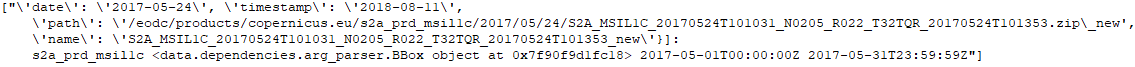
\includegraphics[width=\textwidth]{eva_data_changes_7_state}
	%	\caption{Step 1: State of the re-execution of pidA at the 7th evaluation step.}
	%	\label{fig:eva_data_changes_7_state} % \label has to be placed AFTER \caption (or \subcaption) to produce correct cross-references.
	%\end{figure}
	
	\begin{code}
		\begin{minted}[fontsize=\small]{text} 
[{'timestamp': '2019-03-31 17:44:43', 
'path': '/eodc/products/copernicus.eu/s2a_prd_msil1c/2017/05/24/
S2A_MSIL1C_20170524T101031_N0205_R022_T32TQR_20170524T101353_new.zip'}]
		\end{minted}
		\caption{List of files that replaced original files of the query result.}
		\label{lst:eva_datachange_state}
	\end{code}
	
	\item \textbf{Run duplicate of jobA, by using the data PID of jobA named jobD}\\
	Listing \ref{lst:eva_datachange_8} shows the code of running a new jobD with the data PID pidA. The code is executed after one file is deleted from the resulting file list of pidA. After the creation of the job, the backend notices that the number of result files is different than the first execution of the input data PID. Therefore, a warning message is displayed into the console of the researcher. If the scientist starts the job nevertheless, the backend looks for updated files like described in the previous step and adds the most recent version of the missing file to the query result. It leads to a new data PID for jobD, since the query result has changed. Table \ref{Tab:eva_datachanges5} show the \textit{Query} table status after the execution. The second query entry has a different result hash, since one file changed and therefore, gets a new data PID. 
	\begin{code}
		\begin{minted}[fontsize=\small]{python}
# Take input data of job A by using the input data PID A of job A
pgD = processes.get_data_by_pid(data_pid=pidA)
# Choose processes
pgD = processes.ndvi(pgC, nir="B08", red="B04")
pgD = processes.min_time(pgD)
# Create and start Job D
jobD = con.create_job(pgD.graph)
# Stdout: Warning: The resulting file list changed from the original query
# execution! Look into the "state" attribute to see the list of files that
# have changed. 
jobD.start_job()
pidD = jobD.get_data_pid() # pidD != pidA
		\end{minted}
		\caption{Run duplicate of jobA, by using the data PID of jobA named jobD.}
		\label{lst:eva_datachange_8}
	\end{code}
	
	\begin{table}[]
		\caption{\textit{Query} table after the execution of Listing \ref{lst:eva_datachange_4}. Important elements are highlighted blue if they are the same and red if they are different.}
		\centering
		\begin{tabular}{|r|l|}
			\hline \multicolumn{2}{|c|}{\textbf{Query pidA (full entry in Table \ref{Tab:eva_datachanges1})}} \\
			\hline \multicolumn{1}{|c|}{\textbf{Column}}  &  \multicolumn{1}{c|}{\textbf{Value}} \\ \hline
			query\_pid & {\color{red}qu-a3bbe4a0-a875-4687-bb78-9457f33134a9}  \\ 
			norm\_hash & {\color{blue}0917c7a21cec960b8a6617b22ad26578c2c67f0b0501ba1a359b078c6c51d77d}  \\
			result\_hash & {\color{red}abf43f519007050cbaeb59a067a2226d64b041c6d6ec323b2401109176e66455}   \\
			meta\_data & {'result\_files': 51}  \\
			\hline \multicolumn{2}{|c|}{\textbf{Query pidD}} \\
			\hline \multicolumn{1}{|c|}{\textbf{Column}}  &  \multicolumn{1}{c|}{\textbf{Value}} \\ \hline
			query\_pid & { \color{red} qu-3544aeae-cd24-4b6d-ad34-0d674c2a400f}  \\ 
			dataset\_pid & s2a\_prd\_msil1c  \\ 
			original & see Figure \ref{fig:appendix_pidD} in the appendix \\
			normalized & see Listing \ref{lst:eva_datachange_nq1}  \\
			norm\_hash & {\color{blue}0917c7a21cec960b8a6617b22ad26578c2c67f0b0501ba1a359b078c6c51d77d}  \\
			result\_hash & {\color{red}28088d113de19ce037e9651a64bae3f7957822665f17d8f4e2c7e6b2cf4250b3}  \\
			updated\_at & 2019-03-31 18:10:26.931578   \\
			meta\_data & {'result\_files': 51}  \\
			created\_at & 2019-03-31 18:10:25.46402   \\ \hline
		\end{tabular}
		\label{Tab:eva_datachanges5}
	\end{table}
\end{enumerate}

The result of the second Test Case shows how the backend behaves on data updated that replace the original data. If the file is deleted, the researcher gets a warning message and a list of files that are replacing the original files. Since the path of the file identifies the date and tile that was used, the researcher asks EODC about the concrete changed file. On creation of the new jobD that uses the input data identifier pidA, the user gets notified that the result files changed, before the execution happens. Then the user can decide to start the job nevertheless or contact EODC about the modified files.

\subsection{Test Case 3: Is it possible to re-execute a query after a data file is deleted?}
The deletion of a file without a new file replacing it is not within the policies of EODC since they would restrict their range on available data. If this happens nevertheless, there is in the current solution, no possibility to get the exact removed files. The number of result files in the meta\_data column shows how many files changed. The whole result files need to be added to the \textit{Query} table to achieve the knowledge of missing files. In the current solution, EODC needs to be notified about the missing files. EODC has to look up what files were deleted using the filter arguments of the query to identify the original files and copy them from ESA again. 

%The researcher can query the data at ESA directly with the same filter arguments and can compare the resulting file list with the ones from the re-execution of EODC, but the solution is not doing it automatically.  

%The remaining question is how the system behaves if the data is updated during the query processing. Since there is no permission to perform a test on it, it can only be assumed theoretically. Since the query system is file based and an update results in a new file replacing an existing file. There are two possibilities of the outcome of a query be executed at the same time. Either the query results in the old file, which then will result in an error at the execution if the file is replaced already at the time of the job execution, or the query results in the new file. In both cases the data PID will be generated consistent with the job execution, since it takes the original executed query and the actual file list used for the execution.     
\section{Job Capturing}\label{Evaluation:special_jobcap}

This section reviews the outcome of job capturing. The focus is on the created context model of the job executions. The following question is used to discuss the impact of the captured data regarding job execution.
  \\

\textbf{Is it possible to recreate an older version of the backend?} \\
The implementation aims to capture enough data to make it possible to re-run the same job. The EODC backend is created directly by its GitHub repository. The GitHub repository URL and the commit identifier of the original set up are needed to recreate an old version of the backend. The timestamp of the job execution is persisted in the context model of the first job execution. The backend provenance can resolve the original GitHub repository and commit. Therefore, the information on re-creating the backend state from an older version is captured. The process graph of it is persisted and can be re-executed to re-create the first job on the backend. The execution of the job is the same, assuming the input data has not been deleted in the meantime, which can be checked by re-executing the data query of the job. The resulting hash makes it possible to validate if the job re-execution was the same. The following code presents how this workflow can be achieved in the solution.

\begin{enumerate}
	\item \textbf{Run Job A, which creates query pidA and job\_idA.} \\
	The first step shows the definition, creation, and execution of jobA. The last two lines show how the version can be retrieved from the backend. The "con.version()" method returns the current version of the backend, but can also take a timestamp as a parameter to get the version of that time. The "jobA.get\_backend\_version()" method returns the version of the backend during the execution of jobA. Both versions are at the end of Step 1 identical. 
	\begin{code}
		\begin{minted}[fontsize=\small]{python}
import openeo
# Connect with GEE backend
con = openeo.connect("http://openeo.local.127.0.0.1.nip.io")
# Choose dataset
processes = con.get_processes()
pgA = processes.get_collection(name="s2a_prd_msil1c")
pgA = processes.filter_daterange(pgA, extent=["2017-05-01", "2017-05-31"])
pgA = processes.filter_bbox(pgA, west=10.288696, south=45.935871, 
east=12.189331, north=46.905246, crs="EPSG:4326")
# Choose processes
pgA = processes.ndvi(pgA, nir="B08", red="B04")
pgA = processes.min_time(pgA)
# Create and start job A
jobA = con.create_job(pgA.graph)
jobA.start_job()
# Get current backend version
version_old = con.version()
# Get backend version of jobA 
versionA = jobA.get_backend_version()
		\end{minted}
		\caption{Step 1: Researcher runs Job A and gets the used backend version.}
		\label{lst:eva_jobcapture_1}
	\end{code}
	
	\begin{code}
		\begin{minted}[fontsize=\small]{json}
{'branch': 'master',
'commit': '1a0cefd25c2a0fbb64a78cd9445c3c9314eaeb5b',
'url': 'https://github.com/bgoesswein/implementation_backend.git'}
		\end{minted}
		\caption{Step 1: Version of the jobA execution version\_old.}
		\label{lst:eva_jobcapture_1_1}
	\end{code} 
	
	\item \textbf{Publish job\_idA and pidA.} \\
	The researcher can get the persistent input data identifier pidA and the job identifier jobA\_id to cite the provenance of the execution. The timestamp of the execution in the context model can be used to identify the backend version used for the calculation.
	\begin{code}
		\begin{minted}[fontsize=\small]{python}
# Get input data PID of jobA 
pidA = jobA.get_data_pid()
jobA_id = jobA.job_id
		\end{minted}
		\caption{Researcher gets the input data PID of jobA and the job\_id of jobA.}
		\label{lst:eva_jobcapture_2}
	\end{code}
	
	\item \textbf{Update backend version} \\
	In this step, the backend gets modified slightly by updating a python package to the requirements file of the job execution. The file gets edited by replacing the line "urllib3==1.23" with "urllib3==1.24.1". After editing the file the "git commit" command gets called. 
	\item \textbf{Get original context of jobA} \\
	Listing \ref{lst:eva_jobcapture_4} shows the code the researcher has to run to get the original version of the jobA execution. The variable "versionA" is containing the same version that is displayed in Listing \ref{lst:eva_jobcapture_1_1}. 
	\item \textbf{Re-run jobA with the original version.} \\
	To get the original version of the backend, EODC has to create a second instance of the backend. Then EODC has to check out the commit of the job execution version, by running "git checkout commit\_id" in the console, where "commit\_id" is the value of "versionA["commit"]".
	\begin{code}
		\begin{minted}[fontsize=\small]{python}
import openeo
# Connect with GEE backend
con = openeo.connect("http://openeo.local.127.0.0.1.nip.io")
# Get jobA using the jobA_id.
jobA = con.get_job(jobA_id)
# Get the version of the backend that was active during the job A execution
versionA = jobA.get_backend_version()
		\end{minted}
		\caption{Researcher gets the original backend version of the jobA execution.}
		\label{lst:eva_jobcapture_4}
	\end{code}	
	
\end{enumerate}

\section{Performance and Storage Impact}\label{Evaluation:impact}

This section evaluates the performance and storage impact of the implementation of the EODC backend. 18 input process graphs from 9 publications that used data provided by EODC from the last two years are defined to achieve that. The data used in the papers provide spatial and temporal extents. These 18 input process graphs represent the 18 test cases, Table \ref{Tab:appendix} shows the papers used for the test cases. The evaluation code (evaluation\_impact.py) contains the values of the spatial and temporal extent. The performance of the solution backend is compared to a local EODC backend, without the extensions of this thesis (from now on referred to as "reference backend"). Note that in the reference backend the processing is mocked up in the same way as the solution system. Figure \ref{fig:experiment_overview} gives an overview of the evaluation setup.  

\begin{figure}[h]
	\centering
	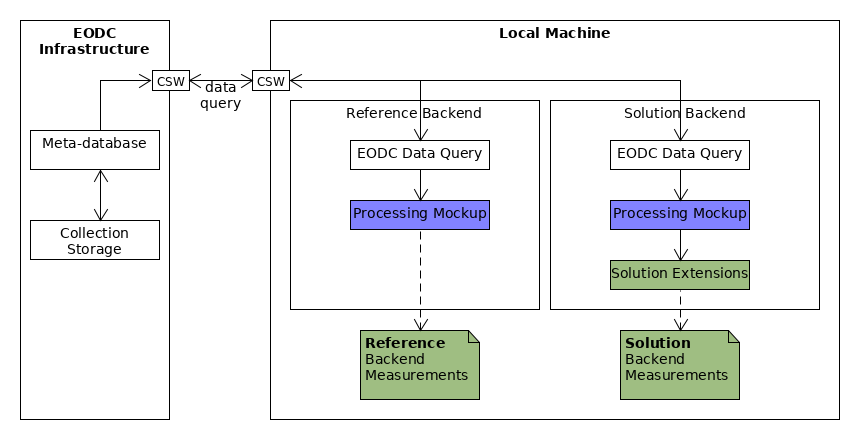
\includegraphics[scale=0.5]{experiment_overview}
	\caption{Overview of the evaluation setup.}
	\label{fig:experiment_overview} % \label has to be placed AFTER \caption (or \subcaption) to produce correct cross-references.
\end{figure}

\begin{table}[]
	\caption{List of geoscientific papers used for the input data of the impact evaluation in Section \ref{Evaluation:Setup}}
	\centering
	\begin{tabular}{c|c|c}
		\textbf{Test Cases} & \textbf{DOI} & \textbf{Citation}  \\ \hline
		1 & 10.1080/01431160902887339 & \cite{evaluation1} \\ 
		2-4 & 10.3390/rs8050402 & \cite{evaluation2} \\ 
		5,6 & 10.1016/j.jag.2014.12.001  & \cite{evaluation3} \\
		7 & 10.1016/j.jag.2016.12.003  & \cite{evaluation4} \\
		8 & 10.3390/rs8110938  & \cite{evaluation5} \\
		9 & 10.1080/2150704X.2016.1225172  & \cite{evaluation6} \\
		10-13 & 10.1109/TGRS.2018.2858004  & \cite{evaluation7} \\
		14 & 10.1080/01431161.2018.1479788  & \cite{evaluation8} \\
		15-18 & 10.3390/rs10071030  & \cite{evaluation9} \\
	\end{tabular}
	\label{Tab:appendix}
\end{table}

\subsection{Performance}\label{Evaluation:impact_perf}

In this section, we evaluate the performance impact on the EODC backend by measuring the difference of job execution durations between the reference backend and the solution backend. The execution time of the implementation is measured by writing timestamps into a log file and calculating the duration afterward. Duration of the \textit{Query Handler} (see Section \ref{Implementation:Data Identification}) execution is measured, as well as the duration of the context model creation process (described in Section \ref{Implementation:Job dependent provenance}). Every test case is executed 50 times at each backend. Before each test case execution, the backend gets cleaned up, so that each iteration happens in the same backend conditions. 

\subsubsection{Performance of Query Handler}\label{Evaluation:impact_perf_query}
This section provides for each element of the \textit{Query} table a description regarding the performance constraints.

\begin{itemize}
	\item \textbf{dataset\_pid} \\
	The dataset\_pid is taken directly from the parsed filter arguments of EODC and has, therefore, a complexity of $O(1)$. Figure \ref{fig:evaluation_perf_datapid} shows the performance results, which are between 4 µs and 26 µs with a median of 8 µs. The boxplot shows that the duration time of retrieving the dataset PID is, except for a view aberrations, similar between all test case executions and independent of the job configuration.
	\begin{figure}[!h]
		\centering
		\caption{Boxplot of the duration needed in the test cases to handle the data PID entry. }
		\label{fig:evaluation_perf_datapid}
		\begin{tikzpicture}
		\begin{axis}
		[
		xlabel={duration [µs]},
		y=2cm,
		ytick={1},
		yticklabels={dataset\_pid},
		]
		\addplot+[
		boxplot prepared={
			lower whisker=4,
			lower quartile=6,
			median=8,
			upper quartile=9,
			upper whisker=26,
			box extend=1,
			whisker extend=0.5,
		},
		] coordinates {};
		\end{axis}
		\end{tikzpicture}
	\end{figure}
	\item \textbf{original} \\
	The \textit{Query Execution} component of EODC passes the original query. The \textit{Query Handler} transforms the query into a string. The query string has the same size for each query, and just the argument values are exchanged. Therefore it has a complexity of $O(1)$. The execution time of the test cases is between 24 µs and 98 µs, with a median of 37 µs during the test cases. Figure \ref{fig:evaluation_perf_original} shows the box-plot of all test case executions and therefore the distribution of duration. It shows that most of the original query retrieval time is in a small range. The duration of the first query execution is constant in time and independent on the job configuration. 
	\begin{figure}[!h]
		\centering
		\caption{Boxplot of the duration time of the test cases to handle the original query entry.}
		\label{fig:evaluation_perf_original}
		\begin{tikzpicture}
		\begin{axis}
		[
		xlabel={duration [µs]},
		y=2cm,
		ytick={1},
		yticklabels={original},
		]
		\addplot+[
		boxplot prepared={
			lower whisker=24,
			lower quartile=29,
			median=37,
			upper quartile=45,
			upper whisker=98,
			box extend=1,
			whisker extend=0.5,
		},
		] coordinates {};
		\end{axis}
		\end{tikzpicture}
	\end{figure}
	\item \textbf{normalized} \\
	The normalized query is the result of an alphabetical sorting of the parsed filter arguments of EODC. The sorting takes nearly constant duration time, since there are only 4 filter arguments allowed in the openEO API version 0.3.1, but they may not all be used. The sorting algorithm has a complexity of $O(n\log{}n)$, where n is the number of crucial elements in the dictionary (amount of filter operations). In this evaluation, four filter arguments were used for each test case. Therefore it has a constant complexity for each test case. In the test cases, it takes between 38 µs and 132 µs with a median of 59 µs of duration time. Figure \ref{fig:evaluation_perf_normalized} shows the box-plot of all test case executions to visualize that the execution time is not spread widely.  
	\begin{figure}[!h]
		\centering
		\caption{Boxplot of the duration time of the test cases to handle the normalized query entry.}
		\label{fig:evaluation_perf_normalized}
		\begin{tikzpicture}
		\begin{axis}
		[
		xlabel={duration [µs]},
		y=2cm,
		ytick={1},
		yticklabels={normalized},
		]
		\addplot+[
		boxplot prepared={
			lower whisker=38,
			lower quartile=47,
			median=59,
			upper quartile=75,
			upper whisker=132,
			box extend=1,
			whisker extend=0.5,
		},
		] coordinates {};
		\end{axis}
		\end{tikzpicture}
	\end{figure}
	\item \textbf{norm\_hash} \\
	The performance of the normalized query hash is dependent on the size of the normalized query ($O(n)$, where n is the size of the normalized query string). In this evaluation, it is constant since in every test case, there are four filter arguments used, which makes the normalized query have a constant length. In the test cases, the duration is between 15 µs and 54 µs with a median of 20 µs. Figure \ref{fig:evaluation_perf_norm_hash} shows the box-plot of all test case executions. Except for a view exceptions the duration has a small range of distribution. It shows the distribution of the duration, which is independent on the job configuration. 
	\begin{figure}[!h]
		\centering
		\caption{Boxplot of the duration time of the test cases to handle the normalized query hash entry.}
		\label{fig:evaluation_perf_norm_hash}
		\begin{tikzpicture}
		\begin{axis}
		[
		xlabel={duration [µs]},
		y=2cm,
		ytick={1},
		yticklabels={norm\_hash},
		]
		\addplot+[
		boxplot prepared={
			lower whisker=15,
			lower quartile=17,
			median=20,
			upper quartile=25,
			upper whisker=54,
			box extend=1,
			whisker extend=0.5,
		},
		] coordinates {};
		\end{axis}
		\end{tikzpicture}
	\end{figure}
	\item \textbf{result\_hash} \\
	Duration of the result hash creation is dependent on the length of the resulting file list. The SHA-256 operation has a complexity of $O(n)$, where n is the length of a resulting file list string. In the test cases, the duration time of the result hash calculation is between 28 µs and 9167 µs with a median of 51 µs. Figure \ref{fig:evaluation_data_resulthash} shows the duration of the result hash creation of the test cases, sorted by the size of the result file set in an ascending way. The data of the chart is in Table \ref{Tab:data_result_hash}, which shows the relationship between the number of files and average duration time of the test cases.  
	
	\begin{table}[]
		\caption{Result hash performance of the test cases depending on the number of result files.}
		
		\centering
		\begin{tabular}{c|c|c}
			\textbf{Test Case} & \textbf{Number of files} & \textbf{Result hash duration [µs]}  \\ \hline
			1 & 14  & 47.244 \\ \hline 
			2 & 24 & 78.047 \\ \hline
			3 & 11 & 37.209 \\ \hline
			4 & 9 & 32.419 \\ \hline
			5 & 10 & 35.000 \\ \hline
			6 & 10 & 35.884 \\ \hline
			7 & 10 & 33.818 \\ \hline
			8 & 12 & 36.886 \\ \hline
			9 & 2255 & 8698.7 \\ \hline
			10 & 17 & 59.359 \\ \hline
			11 & 1551 & 5343.588 \\ \hline
			12 & 12 & 41.548 \\ \hline
			13 & 28 & 95.182 \\ \hline
			14 & 420 & 1400.707 \\ \hline
			15 & 15 & 50.146 \\ \hline
			16 & 1356 & 4985.047 \\ \hline
			17 & 15 & 51.565 \\ \hline
			18 & 54 & 187.186 \\ 
		\end{tabular}
		\label{Tab:data_result_hash}
	\end{table}
	
	\begin{figure}[h]
		\centering
		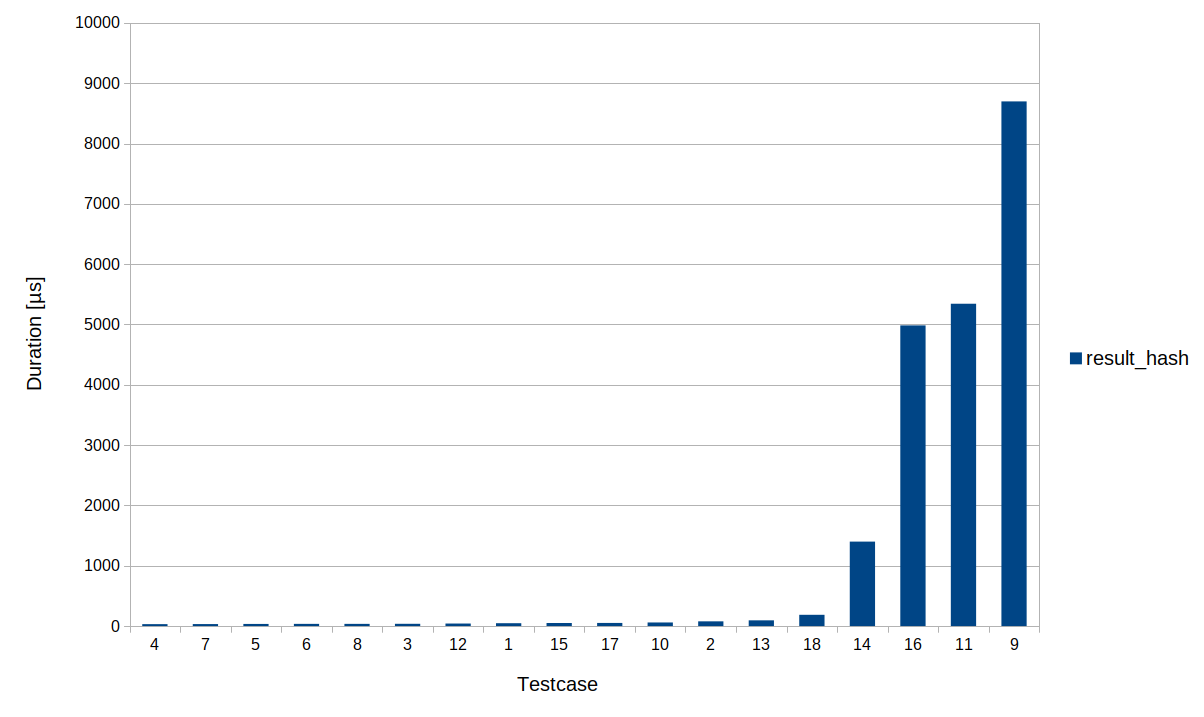
\includegraphics[scale=0.45]{eva_data_resulthash}
		\caption{Execution duration of the test cases, ascending sorted by result size.}
		\label{fig:evaluation_data_resulthash} % \label has to be placed AFTER \caption (or \subcaption) to produce correct cross-references.
	\end{figure}
	
	%	\begin{figure}[h]
	%		\centering
	%		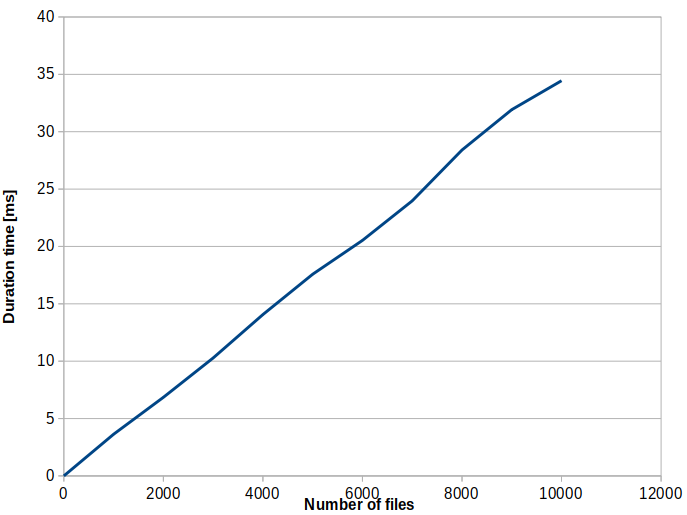
\includegraphics[scale=0.35]{evaluation_impact_data_resulthash}
	%		\caption{Execution duration of the sha-256 over the test cases.}
	%		\label{fig:evaluation_impact_data_resulthash} % \label has to be placed AFTER \caption (or \subcaption) to produce correct cross-references.
	%	\end{figure}
	\item \textbf{meta\_data} \\
	The data in the implementation is the number of result files. It is measured by the built-in len() operator in python, which has a complexity of $O(1)$ according to the official python description\footnote{https://wiki.python.org/moin/TimeComplexity}. In the test cases, the data calculation takes a duration between 6 µs and 359 µs with a median of 12 µs. Figure \ref{fig:evaluation_perf_meta_data} shows the box-plot of the test case execution.
	\begin{figure}[!h]
		\centering
		\caption{Boxplot of the duration time of the test cases to handle the meta\_data entry.}
		\label{fig:evaluation_perf_meta_data}	
		\begin{tikzpicture}
		\begin{axis}
		[
		xlabel={duration [µs]},
		y=2cm,
		ytick={1},
		yticklabels={meta\_data},
		]
		\addplot+[
		boxplot prepared={
			lower whisker=6,
			lower quartile=10,
			median=12,
			upper quartile=17,
			upper whisker=359,
			box extend=1,
			whisker extend=0.5,
		},
		] coordinates {};
		\end{axis}
		\end{tikzpicture}
	\end{figure}
	\item \textbf{Database operations} \\
	To ensure that there are no duplicate query entries in the database, the \textit{Query Handler} executes a SQL SELECT statement to check if there is already an entry with the same normalized query hash and the same result hash. In the evaluation, the \textit{Query} table is empty before the SELECT statement. Hence the complexity is $O(1)$. The INSERT statement to store the query has a complexity of $O(1)$. The database operations in the test cases take between 10.501 ms and 49.283 ms with a median of 13.377 ms duration time. Figure \ref{fig:evaluation_perf_data_database} shows the box-plot of the test case executions.  
	\begin{figure}[!h]
		\centering
		\caption{Boxplot of the duration time of the test cases to make the needed database operations.}
		\label{fig:evaluation_perf_data_database}	
		\begin{tikzpicture}
		\begin{axis}
		[
		xlabel={duration [ms]},
		y=2cm,
		ytick={1},
		yticklabels={database operations},
		]
		\addplot+[
		boxplot prepared={
			lower whisker=10.501,
			lower quartile=11.837,
			median=13.377,
			upper quartile=16.680,
			upper whisker=49.283,
			box extend=1,
			whisker extend=0.5,
		},
		] coordinates {};
		\end{axis}
		\end{tikzpicture}
	\end{figure}
\end{itemize}

Figure \ref{fig:eva_data_static} show the duration of the constant query elements of the different test cases. The test cases are sorted by the result size in ascending order.

\begin{figure}[h]
	\centering
	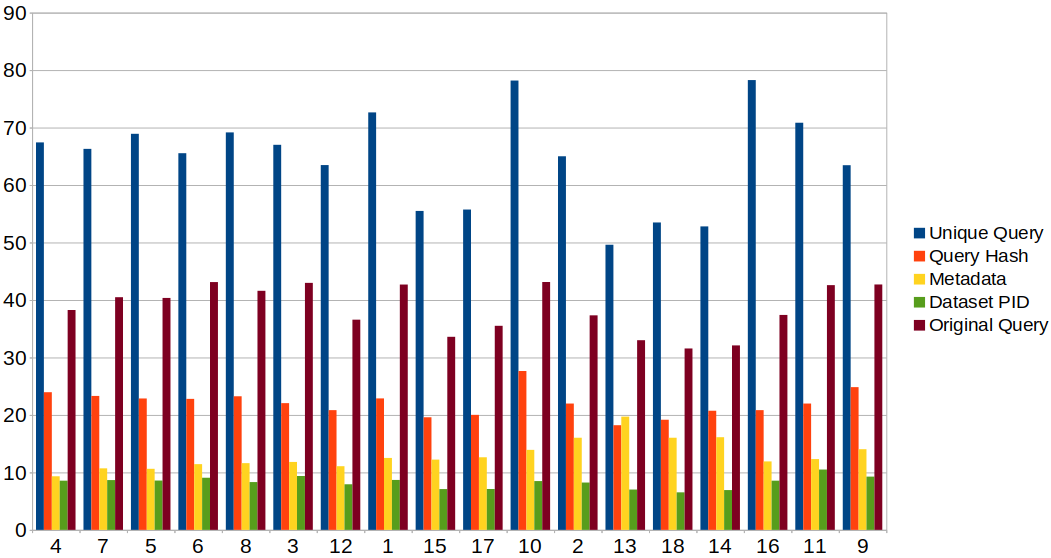
\includegraphics[scale=0.55]{eva_data_static}
	\caption{Constant elements of the \textit{Query Handler} calculation in relation to the test cases sorted by result size.}
	\label{fig:eva_data_static} % \label has to be placed AFTER \caption (or \subcaption) to produce correct cross-references.
\end{figure}


\subsubsection{Performance of Context Model Creation}\label{Evaluation:impact_perf_context}

\begin{enumerate}
	\item \textbf{Constant context model elements} \\
	The following elements of the context model are constant in duration time: the programming language, the input data identifier, the backend version, and the start and end timestamp. These are independent of the job configuration and are read operations with a complexity of $O(1)$. The constant context model elements in the test cases take a duration time between 26 µs and 122 µs with a median of 41.5 µs. Figure \ref{fig:evaluation_perf_static_cm} shows the box-plot of the test case execution.
	\begin{figure}[!h]
		\centering
		\caption{Box-plot of the duration time of the test cases to handle the constant context model elements.}
		\label{fig:evaluation_perf_static_cm}		
		\begin{tikzpicture}
		\begin{axis}
		[
		xlabel={duration [µs]},
		y=2cm,
		ytick={1},
		yticklabels={Constant Elements},
		]
		\addplot+[
		boxplot prepared={
			lower whisker=26,
			lower quartile=34,
			median=41.5,
			upper quartile=47,
			upper whisker=122,
			box extend=1,
			whisker extend=0.5,
		},
		] coordinates {};
		\end{axis}
		\end{tikzpicture} 
	\end{figure}
	\item \textbf{Dependencies of the programming language} \\
	A "pip freeze" execution retrieves the dependencies of the EODC backend. It is independent on the complexity of the job, hence has a constant duration time. The duration in the test cases executions is between 92 µs and 289 µs with a median of 133 µs. Figure \ref{fig:evaluation_perf_python} shows the box-plot of the test case execution.
	\begin{figure}[!h]
		\centering
		\caption{Box-plot of the duration time of the test cases to retrieve the modules of python.}
		\label{fig:evaluation_perf_python}		
		\begin{tikzpicture}
		\begin{axis}
		[
		xlabel={duration [µs]},
		y=2cm,
		ytick={1},
		yticklabels={python modules},
		]
		\addplot+[
		boxplot prepared={
			lower whisker=92,
			lower quartile=112,
			median=133,
			upper quartile=150.5,
			upper whisker=289,
			box extend=1,
			whisker extend=0.5,
		},
		] coordinates {};
		\end{axis}
		\end{tikzpicture}
	\end{figure}
	\item \textbf{Result hash} \\
	The duration of the resulting hash is dependent on the length of the resulting image. The SHA-256 operation has a complexity of $O(n)$, where n is the size of the output image. In the test cases, the duration time of the result hash calculation is between 1.924 ms and 106.270 ms with a median of 2.521 ms. Table \ref{Tab:result_hash} shows the test cases and their result size concerning the average duration time of the result hash calculation. In the experiment setup, every 100 kByte of output data resulted in average in an additional duration of 371 µs. The test cases 9, 11, 14, and 16 had the most prominent result file and therefore needed the most time in the result hash calculation.     
	
	\begin{table}[]
		\centering
		\caption{Result hash performance of the test cases depending on the result size.}
		\begin{tabular}{c|c|c}
			\textbf{Test Case} & \textbf{Result size [kByte]} & \textbf{Result hash duration [ms]}  \\ \hline
			1 & 587  & 2.184 \\ \hline 
			2 & 721 & 2.684 \\ \hline
			3 & 600 & 2.233 \\ \hline
			4 & 556 & 2.068 \\ \hline
			5 & 570 & 2.119 \\ \hline
			6 & 553 & 2.058 \\ \hline
			7 & 578 & 2.149 \\ \hline
			8 & 638 & 2.374 \\ \hline
			9 & 27 999 & 104.182 \\ \hline
			10 & 621 & 2.313 \\ \hline
			11 & 7 969 & 29.654 \\ \hline
			12 & 649 & 2.415 \\ \hline
			13 & 1 376 & 5.121 \\ \hline
			14 & 6 026 & 22.422 \\ \hline
			15 & 777 & 2.891 \\ \hline
			16 & 7 978 & 29.685 \\ \hline
			17 & 733 & 2.727 \\ \hline
			18 & 706 & 2.627 \\ 
		\end{tabular}
		\label{Tab:result_hash}
	\end{table}
	
	\item \textbf{Database UPDATE operation} \\
	The job entry gets updated to store the context model in the database by an SQL UPDATE statement. It is independent on the job configuration. The duration time at the test case execution is between 3.631 ms and 20.099 ms, with a median of 5.493 ms. Figure \ref{fig:evaluation_perf_database} shows the box-plot of the test case execution. 
	
	\begin{figure}[!h]
		\centering
		\caption{Box-plot of the duration time of the test cases to retrieve the modules of python.}
		\label{fig:evaluation_perf_database}		
		\begin{tikzpicture}
		\begin{axis}
		[
		xlabel={duration [ms]},
		y=2cm,
		ytick={1},
		yticklabels={UPDATE operation},
		]
		\addplot+[
		boxplot prepared={
			lower whisker=3.631,
			lower quartile=4.595,
			median=5.493,
			upper quartile=7.237,
			upper whisker=20.099,
			box extend=1,
			whisker extend=0.5,
		},
		] coordinates {};
		\end{axis}
		\end{tikzpicture}
	\end{figure}
	
\end{enumerate}

The context model creation performance is not affected much by the complexity of the test cases. The captured data for the context model is not related to the complexity of the execution. The "Increase" column of Table \ref{Tab:eva_performance} shows that simple test cases are affected the most in terms of relative performance loss because the \textit{Query Handler} and the context model have elements that need the same duration time independent of the test case configuration. In conclusion, it can be seen that the execution of the \textit{Query Handler} and the context model is less affecting complex test cases since there is a minimum duration time needed for the data creation and just a small additional duration time depending on the size for the resulting files. Besides, it should be mentioned that the \textit{Query Handler} and the context model creation happens after the processing. So that the result files of the job execution can be accessed by the user even if both modules have not finished yet. \\
Table \ref{Tab:eva_performance} summarizes the result of the mean duration time of the 50 runs of each the test case. The second column presents the duration of the reference backend. The other columns are measurements of the solution system. Including the total execution duration of the solution, the duration of the \textit{Query Handler} and the duration of the context model creation. The last column consists of the additional time that the solution systems needs in comparison to the reference system. The last row of the table shows the mean duration overall test cases. It shows that the solution adds between 20 ms and 175 ms to the reference backend, depending on the result sizes and not on the execution duration of the processing. Compared to the estimated computation time of the test cases between 10 seconds and 20 minutes at the production version of the EODC backend, we conclude that the impact of the Query Handler is negligible.

\begin{table}[]
	\caption{Mean duration time over 50 runs of the solution and the reference backend by executing the test cases}
	\begin{tabular}{r|r|r|r|r|r}
		
		\textbf{} & \textbf{Reference Backend} & \multicolumn{3}{c|}{\textbf{Solution Backend}} &  \\ \hline \textbf{Test} & \textbf{} & \textbf{Comparison} & \textbf{Query} & \textbf{Context} & \textbf{Solution} \\ 
		\textbf{Case} & \textbf{Total} & \textbf{Total} & \textbf{Handler} & \textbf{Model} & \textbf{Addition} \\ \hline
		1 & 322.946 ms & 345.127 ms & 14.187 ms & 7.994 ms & 22.181 ms \\ 
		2 & 369.066 ms & 393.505 ms & 16.342 ms & 8.097 ms & 24.439 ms \\ 
		3 & 281.657 ms & 305.407 ms & 15.669 ms & 8.081 ms & 23.750 ms \\ 
		4 & 276.324 ms & 298.954 ms & 14.015 ms & 8.615 ms & 22.630 ms \\ 
		5 & 312.150 ms & 334.802 ms & 13.925 ms & 8.727 ms & 22.652 ms \\ 
		6 & 314.571 ms & 337.290 ms & 13.985 ms & 8.734 ms & 22.719 ms \\ 
		7 & 320.081 ms & 343.552 ms & 14.555 ms & 8.916 ms & 23.471 ms \\ 
		8 & 304.998 ms & 328.633 ms & 14.742 ms & 8.893 ms & 23.635 ms \\ 
		9 & 565.289 ms & 740.751 ms & 48.766 ms & 126.696 ms & 175.462 ms \\ 
		10 & 401.922 ms & 425.026 ms & 14.874 ms & 8.230 ms & 23.104 ms \\ 
		11 & 521.022 ms & 605.185 ms & 34.660 ms & 49.503 ms & 84.163 ms \\ 
		12 & 387.536 ms & 412.079 ms & 15.711 ms & 8.832 ms & 24.543 ms \\ 
		13 & 510.517 ms & 538.784 ms & 17.070 ms & 11.197 ms & 28.267 ms \\ 
		14 & 657.989 ms & 706.329 ms & 19.010 ms & 29.330 ms & 48.340 ms  \\ 
		15 & 345.806 ms & 371.984 ms & 17.027 ms & 9.151 ms & 26.178 ms \\ 
		16 & 585.730 ms & 658.493 ms & 23.956 ms & 48.807 ms & 72.763 ms \\ 
		17 & 563.755 ms & 589.776 ms & 16.778 ms & 9.243 ms & 26.021 ms \\ 
		18 & 836.377 ms & 862.271 ms & 16.801 ms & 9.093 ms & 25.894 ms \\ \hline
		\textbf{Avg.} & \textbf{437.652 ms} & \textbf{477.664 ms} & \textbf{19.004 ms} & \textbf{21.008 ms} & \textbf{40.012 ms} \\ 
	\end{tabular}
	\label{Tab:eva_performance}
\end{table}

% The result hash is the only element that is dependent on the complexity of the test case. Most of the complexity comes from the temporal extent of the test cases, which do not affect the size of the resulting file. The reason for this is that the output file is always a composite of the values throughout the time range.

\subsection*{Storage}\label{Evaluation:impact_stor}
This section describes the storage needed for the captured data. Since all the captured data is in the PostgreSQL database, the storage needed by it can be estimated using the PostgreSQL interface. Listing \ref{lst:eva_imact_1} presents the commands used to get the size of the database entries. The id of the data record is inserted into "''" (e.g. job id in the first one).  

\begin{listing}[ht]
	\begin{minted}[fontsize=\small]{sql}
-- Context Model 
SELECT sum(pg_column_size(context_model)) as filesize, count(*) as filerow 
FROM jobs as t WHERE id = '{}';
-- Query Table
SELECT sum(pg_column_size(t)) as filesize, count(*) as filerow 
FROM query as t WHERE query_pid = '{}';
-- QueryJob Table
SELECT sum(pg_column_size(t)) as filesize, count(*) as filerow 
FROM queryjob as t WHERE job_id = '{}';
	\end{minted}
	\caption{PostgreSQL commands to get the size of one data record in the tables job, query and queryob.}
	\label{lst:eva_imact_1}
\end{listing}	

%\begin{table}[]
%\caption{Mean storage over 50 runs of the solution by executing the test cases. All measured %values are in Bytes.}
%\centering
%\begin{tabular}{r|r|r|r|r}

%\textbf{Test Case} & \textbf{Context Model} & \textbf{Query} & \textbf{QueryJob} & \textbf{Sum}
%\\ \hline
%		1 & 1043 & 1529.659 & 113 & 2685.659 \\ 
%		2 & 1043 & 1530.583 & 113 & 2686.583 \\ 
%		3 & 1043 & 1525.585 & 113 & 2681.585 \\ 
%		4 & 1043 & 1533.649 & 113 & 2689.649 \\ 
%		5 & 1043 & 1524.622 & 113 & 2680.622 \\ 
%		6 & 1043 & 1520.267 & 113 & 2676.267 \\ 
%		7 & 1043 & 1524.800 & 113 & 2680.800 \\ 
%		8 & 1043 & 1527.614 & 113 & 2683.614 \\ 
%		9 & 1043 & 1532.814 & 113 & 2688.814 \\ 
%		10 & 1043 & 1523.184 & 113 & 2679.184 \\ 
%		11 & 1043 & 1530.667 & 113 & 2686.667 \\ 
%		12 & 1043 & 1524.825 & 113 & 2680.825 \\ 
%		13 & 1043 & 1529.923 & 113 & 2685.923 \\ 
%		14 & 1043 & 1525.614 & 113 & 2681.614 \\ 
%		15 & 1043 & 1524.683 & 113 & 2680.683 \\ 
%		16 & 1043 & 1530.422 & 113 & 2686.422 \\ 
%		17 & 1043 & 1524.846 & 113 & 2680.846 \\ 
%		18 & 1043 & 1521.432 & 113 & 2677.432 \\ \hline
%		\textbf{All} & \textbf{1043} & \textbf{1526.955} & \textbf{113} & \textbf{2682.955} \\
%	\end{tabular}
%	\label{Tab:eva_storage}
%\end{table}

The resulting storage need for the evaluation is quite constant. The mean storage of the 50 runs per test case, and the average storage size of all test cases are calculated. Three parts of the implementation are storing additional information. First, the context model is stored in an additional column named "context\_model" in the \textit{Job} table. There is no element in the context model that can vary in size, except for the list of packages of python, which has not changed during the evaluation. It results in an additional size of 1.043 kByte for each job entry. The same occurs at the \textit{QueryJob} table, which maps the \textit{Query} table and the \textit{Job} table and therefore contains the needed identifiers and timestamps for creation and modification. Every record of the \textit{QueryJob} table needs 0.113 kBytes of storage space.
The Query data records have a varying size because of the string length of the parameters in the original query. The remaining parts of the \textit{Query} table are constant in storage usage — each Query record of the test cases needs between 1.520 kByte and 1.533 kByte storage. The original query makes up the most size needed in the \textit{Query} table (e.g. 959 Bytes of 1521.432 Bytes in Testcase 18), because of the XML annotations. In summary, the average additional storage needed by the reference backend per Job with a new Query entry is 2.677 kBytes. If the used query is already in the \textit{Query} table, only an additional 1.043 kBytes of storage is needed by the solution.

\section{Summary}
The evaluation in this chapter showed how the solution tackles the goals of the research questions. First, it summarizes how the RDA recommendations are implemented in the solution, except for the migration recommendations (R14 and R15). The data identification implementation is then tested against exceptional test cases regarding data updates and data deletions at the backend. The evaluation shows that the solution can re-execute queries properly by returning old versions of updated files. The test cases show that the usage of the data PID as input data of a new job is superior to the current way of re-executing a job with the same process graph at EODC.
The reason for this is that the process graph does not have the original execution timestamp and therefore, does not use the same input data after an update occurs. In the evaluation of deleted data at the backend, the solution happens to be not capable of showing the exact missing files, since not the whole file list result of the query is persisted. The test case on job capturing showed that the solution is capable of identifying the backend version and therefore, the environment of the job execution. Still, to run a new job in the same environment, EODC has to provide it manually. The evaluation also contains a section about the performance and storage impact on the EODC backend, by running 18 test cases derived from past publications that used data from EODC. The results show that, except for the result hashes, the calculation of the data identification and the context model are independent of the complexity of the job. The time of the result hashing used for the data identification is dependent on the size of the query result, and the resulting hash of the context model is dependent on the size of the output file of the job execution. The evaluation of storage impact results in the conclusion that the additional needed space per job is unrelated to the job configuration. It depends on if there is a new query entry added to the database or not. The performance impact of the testcase execution is between 20ms and 170ms. Compared to the estimated computation time of the test cases between 10 seconds and 20 minutes at the production version of the EODC backend, we conclude that the impact of the Query Handler is negligible. The additional needed space per job is constant and also minimal if compared to size of data kept at the backend.
   
\chapter{Conclusion and future Work}\label{Conclusion}

\section{Conclusion}
\todo{Always "the backend" not "the EODC backend", just in the first mentioning of the section}
\todo{Remove automated fashion or add a Why? --> Because EODC does not provide a possibility or it has to be done manually by EODC}

\todo{Gesamte Thesis: Present simple \& Past simple and not "could / would" So: we have implemented --> we implemented}
\todo{Gesamte Thesis: Restructure passive sentences}
\todo{Gesamte Thesis:Konsistente Verwendung von Begriffen --> Glossary ?? --> workflow (Beschreibung des Experiments aus sicht des wissenschaftlers), job (Definition des im backend durchgeführten parts), workflow, process graph (technische Beschreibung bzw. Definition des jobs)}
\todo{Gesamte Thesis: Wortwiederholungen sind gut !!}
\todo{Gesamte Thesis: Unnötige Wörter / Sätze weg z.b. briefly, some, also, ...}
\todo{Gesamte Thesis: Kurze einfache Sätze}
\todo{Gesamte Thesis: Eher Reproducibility schreiben in den Allgemeinen Kapiteln, aber in den RQ repeatability schreiben}
\todo{Gesamte Thesis: Software --> Environment / Code ? --> just check correct usage}
In this thesis, the challenges of providing reproducibility in earth observation science have been explored. The solution consists of data identification and code identification for workflows in the context of geosciences. The implementation within the openEO project proves the concept defined in Section \ref{Design}. It makes it clear that reproducibility can be achieved in earth observation workflows by providing data identification and process identification to existing backends. One reason why earth observation researchers lack reproducibility is the additional time needed to achieve it. With the provided solution, researchers can run experiments on their backend of choice and automatically generate a data identifier that other scientists can use in their research. Besides, scientists can cite the version of the backend and describe the execution environment. The captured data in the context model is capable of reproducing experiments. Nevertheless, it is not supported by the EODC backend in an automated fashion. In the case of the openEO project, the solution concludes in suggestions to openEO for all components of the project.  

\subsection{Research questions revisited}\label{research question revisited}
\todo{Update changed RQs !}
\todo{Programming language --> programming language version}
\todo{Redundante Sätze wegstreichen}
\todo{first execution --> original execution}
\todo{Remove "can assumed"}
\todo{data compared --> Data ID or it changes to Context model somehow}
This section revisits the research questions defined in Section \ref{research question} to discuss how the concept design suits the questions.

\begin{itemize}
	\item \textbf{How can an earth observation job re-execution be applied like the initial execution?}
	\begin{itemize}
		\item \textbf{How can the used data be identified after the initial execution?} \\
		The input data is defined by the satellite data identifier and the filter operations used in the workflow. This information with the hash of the resulting file list defines a single query identified by a PID. The query data record consists of the original execution timestamp to enable the retrieval of the same data versions. By assigning persistent identifiers to every unique input data, the data can be accessed after the first execution.   
		\item \textbf{How can the used software of the initial execution be reproduced?} \\
		The original software is defined by the used code, the programming language, and the installed libraries. In the implementation, Git and GitHub are used to identify and persist the used code version. The version of the programming language and the installed packages are stored in the context model. The backend has to recreate the captured versions of code and state of the programming language to reproduce the first execution.       
		\item \textbf{What data has to be captured when?} \\
		The input data has to be captured at the query execution of the backend to ensure the equality of the persisted query and the first execution. The capturing of the code version has to be executed at the time of the execution, as well as the environment information of the execution. The hash of the resulting output file is calculated right after the creation of it.   
		\item \textbf{How can the result of a re-execution in future software versions be verified?} \\
		The solution persists a hash of the resulting output file. The result hash value of the re-execution is compared with the original execution output hash. If the hash values are not equal, it can be assumed that the result of the re-execution is different from the first execution.  
	\end{itemize}
	\item \textbf{How can the equality of an earth observation job re-execution results be validated?}
	\begin{itemize}
		\item \textbf{What are the validation requirements?} \\
		The validation requirements are the equality of the captured data. Three parts have to be considered by the validation. First, the persistent input data identifier has to be the same between the two executions. Second, the code version. Third, the hash value of the output file.
		\item \textbf{How can the data be compared?} \\
		The data is compared to the equality of all components of the context model. Every item of the context model is compared with the same item of the re-execution context model. There are only three states at the comparison defined: "EQUAL" or the difference of the context model element.
		\item \textbf{How can changes of the earth observation backend environment be recognized?} \\
		The timestamps of the backend provenance version are used to determine the version of the backend. Changes in job dependent environment result in different entries at the job dependent context model.   
		\item \textbf{How can differences in the environment between the executions be discovered?} \\
		The users can compare two job executions at the backend. A result is a JSON object that consists of all elements of the context model with the result of the comparison. In the resulting JSON, it is evident, which part of the environment differs between the executions and how they are different.
	\end{itemize}
\end{itemize}

\section{Future Work}\label{FutureWork}
\todo{improved --> customized}
\todo{be positive about it, so show what can be improved rather than show that is not working yet...}
This thesis proposed a prototype for applying reproducibility in the openEO project. Still, there are significant issues to be addressed in the development of the openEO project. 
openEO is still evolving until the official end of the project in 2021 and will be continued afterward. Many features have to be defined and may interfere with the concept proposed in this thesis. User defined functions (UDF) are part of the project, but not well defined yet. Reproducing executed UDFs may lead to adaptations of the concept. Another main issue of the openEO project is the billing concept that has to be apply-able to a diverse set of backends. Since the capturing process and the generation of the context model needs resources, it has to be considered in the billing plan of the backends. The growing diversity of the backends applying the openEO standard is a huge challenge to remain the design of the context model suitable in the future. The concept needs to be improved by implementing it on other backend types. \\
In the solution of this work, the data is captured to identify how jobs are executed and to be able to identify the provenance. A step further is a way to apply the reproduction of an already executed job automatically. A finer granularity of the process capturing is a possible addition to the concept, leading to a definition of scalability of the processing capturing. A concept to achieve this is presented in Section \ref{Job:Benchmarking} below.

\subsection{Benchmarking Mode}\label{Job:Benchmarking}

So far, only the capturing of the whole process chain, including input and output data, are described. The general idea (presented in Section \ref{Implementation:Job dependent provenance}) of the job dependent provenance capturing is to capture the input data of the process graph, the whole process graph and the output of the process graph. It is a universal concept the backend providers can agree on since it is not affecting the backend providers implementations much. Moreover, it is capable of giving the user a simple overview of how the results are generated and what the differences between job executions are. The granularity of the capturing can be improved to make the comparison of different execution behaviors more informative. \\
Therefore, the benchmarking context model gets introduced. The idea is that not only the input data of the whole process chain and the output data gets captured, but every data state in between each process. For every process in the process graph the input data, the output data, and the code executing the process get captured. It makes it easier for users to see where in the process chain the execution produced different results.\\ The concept leads to higher implementation and execution costs on the backend side. The effect on the performance of the execution is higher than the standard context model. Whether the implementation of such granularity is doable is highly dependent on the backend implementation. Not every backend might be able to implement this into the backend due to external tools where the execution and results of single processes are not distinguishable. If a backend can support it, the granularity can be more exceptional. In an extreme example, the data and code can be captured for every line in the code. The flexibility of capturing granularity may define the context model design in the future.

\chapter{Appendix}\label{Appendix}

\begin{figure}[h]
	\centering
	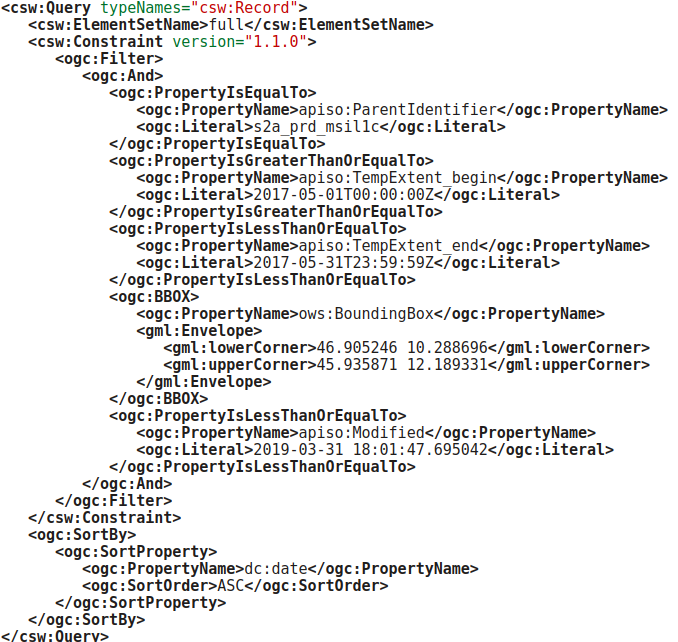
\includegraphics[width=\textwidth]{appendix_pidB}
	\caption{Original query of jobB from the evaluation in Section \ref{Evaluation:special_dataid}.}
	\label{fig:appendix_pidB} % \label has to be placed AFTER \caption (or \subcaption) to produce correct cross-references.
\end{figure}

\begin{figure}[h]
	\centering
	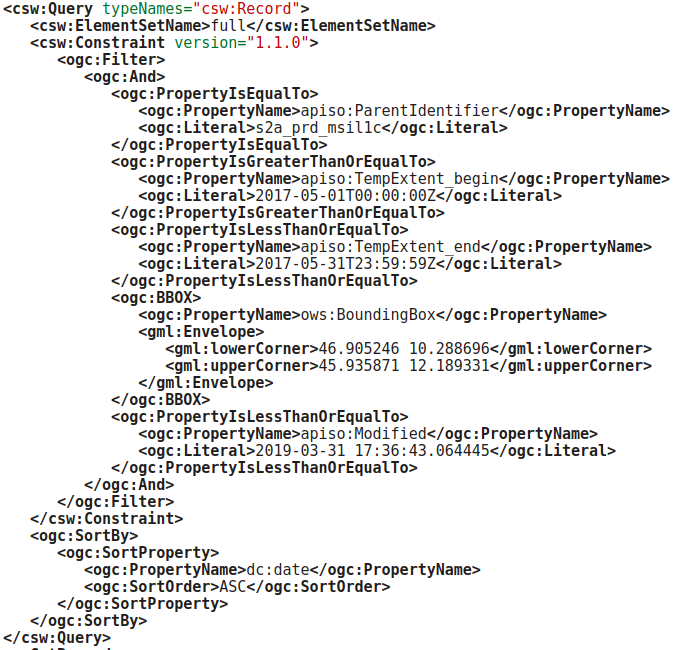
\includegraphics[width=\textwidth]{appendix_pidD}
	\caption{Original query of jobD from the evaluation in Section \ref{Evaluation:special_dataid}.}
	\label{fig:appendix_pidD} % \label has to be placed AFTER \caption (or \subcaption) to produce correct cross-references.
\end{figure}

\backmatter


% Use an optional list of figures.
\listoffigures % Starred version, i.e., \listoffigures*, removes the toc entry.

% Use an optional list of tables.
\cleardoublepage % Start list of tables on the next empty right hand page.
\listoftables % Starred version, i.e., \listoftables*, removes the toc entry.



%\renewcommand\listoflistingscaption{List of source codes}
\listoflistings



% Use an optional list of alogrithms.
%\listofalgorithms
%\addcontentsline{toc}{chapter}{List of Algorithms}

% Add an index.
\printindex

% Add a glossary.
\printglossaries

% Add a bibliography.
\bibliographystyle{abbrv}
\bibliography{intro}

\end{document}